\chapter{The role of vertical structure in QBO teleconnections}
\label{cha:deepQBO}

\section{Introduction}
\label{sec:deepQBO-introduction}

Findings from chapter 3 indicated an association between a vertically integrated QBO index and the vortex (see figures \ref{fig:holton_tan_comp} and \ref{fig:SSW_hist_QBO_phase}). While a large body of work has aimed to understand teleconnections between the equatorial winds and the vortex (see section \ref{sec:external_influence_HT}), aspects of the connection between the QBO and other parts of the stratosphere as well as the troposphere and surface, evade definitive explanation.

The QBO is typically defined by the equatorial ZMZW at a single level in the mid-stratosphere and the 50 hPa level is usually used for observational studies into teleconnections between the QBO and NH variability \citep{baldwinQuasiBiennial2001}. However, some studies have also noted the importance of characterising the vertical structure of the QBO \citep{fraedrichEOF1993, wallaceRepresentation1993,  Baldwin98,  Dunkerton2017, graySurface2018b, andrewsObserved2019d}. In an observational-based study, \cite{graySurface2018b} find an enhanced association between the QBO and polar vortex as well as MSLP anomalies over the NH when a metric incorporating the vertical coherence of equatorial winds via empirical orthogonal functions is utilised. Such an EOF method is first developed in \cite{fraedrichEOF1993} and \cite{wallaceRepresentation1993} and analysed further in \cite{verena2016a}. \cite{graySurface2018b} proposes three distinct physical pathways by which the QBO exerts influence over tropospheric and surface variations: First, via modulation of NH winter vortex strength (the HT effect, see section \ref{sec:external_influence_HT}) and the subsequent downward propagation of NAM anomalies from the vortex to the surface (see section \ref{sec:Downward_influence}). Second, through influence over tropical upwelling that results from the presence of different QBO phases in the lower stratosphere as seen in the observational study of \cite{liessRelationship2012}. Finally, via alterations in horizontal temperature gradients in the tropospheric subtropical jet region also caused by the induced meridional circulation, an effect suggested in \cite{garfinkelInfluence2011}. \cite{graySurface2018b} also shows that the nature of responses in the vortex and surface to the QBO vary significantly within the NH winter season with midwinter responses (in January) sensitive to QBO winds near 50 hPa in contrast to early and later winter (February and March) responses which are most sensitive to the QBO defined at 20 hPa and 70 hPa. In a subsequent model-based study, \cite{andrewsObserved2019d} introduce a similar but simpler methodology by defining the QBO as the average ZMZW between two vertical levels, which preferentially selects time intervals that display a vertically coherent QBO phase between the specified levels. Furthermore, enhanced responses to the QBO from the NAO and the AO are reported (also in \cite{andrewsObserved2019d}) when such vertically integrated metrics are used to define the QBO phase compared to a single level definition. However, the pathways responsible for the enhanced surface response (i.e. whether the vortex response to a deep QBO is also enhanced) and the mechanisms involved in the association are still not well understood. 

In addition to the QBO, variations in the SAO (see section \ref{sec:equatorial_strat}) also show associations with the vortex. The influence of the SAO on vortex variability and SSWs was first hypothesised in the observational study of \cite{grayData2001} which used rocketsonde data to establish a link between the vertical extent of the westerly SAO phase and vortex strength. However, these results were not statistically significant and the work stressed the need for more study with comprehensive observations as well as model simulations. Subsequent studies found similar links but with varying features: \cite{grayinfluence2003} found influence of upper stratosphere equatorial winds and SSWs over the whole season but mostly in mid winter. This was attributed to timing of the phase transition from westerly to easterly SAO. \cite{grayData2001} and \cite{hamiltonEffects1998} suggest that equatorial winds at all stratospheric levels (including the QBO and SAO regions) influence the vortex and a combination of QBO and SAO conditions is required to obtain a significant signal in vortex variability.

While many studies highlight statistical associations between QBO and SAO metrics with other parts of the climate system, they are less effective at demonstrating causal relationships. Indeed, \cite{andrewsObserved2019d} note the possibility that both the occurrence of deep QBO phases and NAO and AO anomalies may be driven by an unidentified third factor which gives rise to a robust statistical link between the phenomena without any direct physical connection. Studies which utilise observation based datasets to examine the QBO-NAO/AO interaction are also hampered by record length as well as the intrusion of other forcing factors associated with NH surface variations which obscure the signal from the QBO. These include Solar cycle variability \citep{GrayElevenyear2016}, volcanic eruptions \citep{stenchikovArctic2004}, in particular stratospheric injection of aerosols, as well as surface variability in other regions such as ENSO \citep{bellStratospheric2009}. Some studies aim to overcome these potential pitfalls and explicitly test the nature of teleconnections with forced model setups, where momentum forcing or nudging is applied to winds in specific regions of the atmosphere. Such works further suggest the importance of the SAO and QBO region when considering the vortex. \cite{pascoeQuasibiennial2005b} finds improved vortex representation in model runs with forced winds in the equatorial stratosphere (both QBO and SAO regions separately) and \cite{grayForecasting2020a} shows that nudging model winds in the SAO region (as well as specifying tropospheric wave forcing) towards reanalysis for a single winter, allows the model to capture an SSW observed in that winter with high degrees of accuracy in its timing and magnitude.   

Despite the significant body of work presented above into the QBO and its relation to other parts of the climate system, the role of vertical structure in teleconnections is not fully understood. In this chapter, we utilise a set of nudging experiments to explicitly test the importance of vertical coherence in the equatorial stratosphere's influence over the vortex as well as tropospheric and surface variability. Results from this analysis may aid in establishing the true nature of QBO teleconnections as well as develop understanding of a potentially powerful source of forecast predictive skill for NH surface weather.

\section{Model configuration}

To explicitly test the effect of QBO vertical coherence on teleconnections, we perform a set of simulations of a modified version of the UKESM GCM analysed in chapters 3 and 4. As with the pi-control simulation examined so far, the model component for the atmosphere is GA7.1, GHG concentrations are set to 1850 levels (see section \ref{sec:model_config}) and volcanic eruptions are absent (however a constant background volcanic aerosol level is imposed). The primary difference between the pi-control and the configuration utilised here is the experiments run with no coupled ocean component. Instead, SSTs are prescribed using monthly mean climatological fields obtained from an interval of the pi-control (year numbers 96-126) \citep{oconnorAssessment2021b}. Sea Ice extents are also prescribed to climatological values using the same interval of the pi-control. All simulations are initialised using conditions from the start of the 30-year interval of the pi-control used to calculate SST and sea ice climatologies (year number 96). We choose to impose SST and sea ice conditions in our experiments as this removes contributions to the NAO/AO from interannual to decadal variability at the surface such as ENSO. The absence of volcanic eruptions similarly prevents influence of stratospheric injection of volcanic aerosols on the NAO. Removing these contributions, in turn, helps to isolate the effects of the QBO on surface variability. We utilise three simulations using the above configuration with different forced setups:

\begin{itemize}
    \item First, an unforced control simulation referred to as the \textbf{pre-industrial clim control} (pi-clim cntrl). This simulation is produced as part of CMIP6 and is run for 45 years. It is documented in full in \cite{oconnorAssessment2021b}. 
    
    \item Second, a forced run which fixes the state of the equatorial winds to a vertically coherent idealised QBO (see next section for details of idealised winds). This simulation is referred to as the \textbf{deep QBO experiment} (or simply the deep experiment) and is run for 50 years.
    
    \item A forced run which fixes the state of the equatorial winds to an idealised QBO with a low degree of vertical coherence (i.e. with opposite phases in the upper and lower stratosphere, see next section). This simulation is referred to as the \textbf{shallow QBO experiment} (or simply the shallow experiment). This simulation is also run for 50 years.
    
\end{itemize}

We choose to simulate both forced runs for 50 years to ensure the simulations cover a sufficient number of the QBO cycles to carry out a robust statistical analysis on QBO teleconnections while also working within restrictions on computing time. The pi-clim cntrl was produced as part of CMIP6 as opposed to created specifically for this analysis and was run for 45 years. This discrepancy in simulation length is relatively small and should not affect the comparison between the experiments. 


%Analysis chapters 4 and 5 showed that this year does not lie in an interval in which the QBO or the vortex exhibits significant multi-decadal oscillations. As a result, the initial conditions for the simulation are less likely samples the QBO and vortex in a randomly chosen state.

\subsection{Nudging}
In order to impose the vertical structure of the QBO in the deep and shallow experiments, we employ a method to constrain atmospheric conditions in a GCM simulation known as nudging. In this method, an atmospheric quantity, $Y$, is constrained via Newtonian-relaxation which pushes the model state for $Y$ towards some imposed value at each model timestep such that

\begin{equation} \label{eq:nudging}
\Delta Y = G \Delta t (Y_{imposed} - Y_{model}), 
\end{equation}

\noindent where $\Delta Y$ is the change in $Y$ applied by the nudging scheme, $Y_{imposed}$ is the state of $Y$ from the imposed field, $Y_{model}$ is the value of $Y$ the model has evolved to since the last timestep (when it was last nudged), $\Delta t$ is the model timestep and $G$ is the relaxation parameter \citep{telfordTechnical2008}. $G$ is a measure of the strength of the relaxation towards $Y_{imposed}$ at each timestep and can also be expressed as $G = \frac{1}{\tau}$ where $\tau$ is known as the relaxation timescale, a measure of speed at which the relaxed field will reach its target value. When choosing the relaxation timescale, a balance is required between constraining the model sufficiently to the imposed state (i.e. a short enough $\tau$ such that the model's $Y$ avoids evolving freely) and avoiding the introduction of large gradients (a large enough $\tau$ to avoid model instability). The MetOffice Unified model, of which the model configurations presented here are a part, typically uses a relaxation timescale of 6 hours at all vertical levels \citep{telfordTechnical2008}. This has been shown to produce good quality nudging results in a range of studies employing such a method despite the different radiative timescales present across atmospheric levels \citep{grayForecasting2020a} so we proceed with this value for our experiments. In our experiments we nudge the zonal wind, $u$, towards an idealised version of the QBO wind fields expressed as 

\begin{equation} \label{eq:imposed_U}
u_{qbo}(t, p) = F(p) sin(\frac{2\pi (t + s(p))}{period}),
\end{equation}

\noindent where $s(p)$ is a parameter which varies with pressure level and sets the rate of phase shift in the QBO with descending height. For simplicity, we choose $s(p)$ such that a linear descent rate with increasing $log(p)$ is achieved. This is achieved by setting $s(p) = k log(p/p_{0})$, where $k$ is a constant and $p_{0}$ is a reference pressure level (in this case 1 hPa) from which we measure the descending phase difference. We then select different values for the parameter $k$ to achieve deep QBO and shallow QBO structures: For the deep experiment, $k = 2.5$ achieves a higher degree of vertical phase coherence while for the shallow experiment, $k = 5$ which leads to a larger phase shift with descending pressure level (and therefore less vertical coherence). The choices of values for this parameter are informed by previous studies into the descent rate of QBO phases. Notably, \cite{kinnersleyDescent1996} and \cite{coySeasonal2020} show in observations that the rate of change of winds with respect to the height coordinate ($z)$, that measures the time variation of vertical shear in the QBO, ranges from approximately $-15-15ms^{-1}km^{-1}$. We therefore aim to reproduce idealised winds with rates of change in this range. We choose the period of the QBO in both experiments to be 32 months for consistency with the QBO period exhibited in the UKESM pi-control which is extended compared to reanalysis (see section \ref{sec:strat_var_UKESM}) as well as that of the pi-clim cntrl which is analysed in the following section. $F(p)$ is a momentum forcing vertical profile applied to reproduce the variation in magnitude of the QBO with pressure level (the QBO peaks in magnitude at around the 20 hPa level in ERA-Interim). We choose our $F(p)$ in line with the methodology of \cite{pascoeQuasibiennial2005b} who design similar idealised QBO fields and utilise a $F(z)$ (with altitude in $km$ as the height coordinate) which takes the form of a Weibull function given by

\begin{equation} \label{eq:vertical_profile}
F(z) = R_D \frac{1}{\gamma \beta^\alpha}  Z_D^{\alpha-1}  e^{-Z_D/\beta},
\end{equation}

\noindent where the parameters are set to $\alpha = 3.5, \beta = 0.27, \gamma = 3.2335, R_D = 40.0 ms^{-1}, Z_{D} = (z - 15)/20$ and we make an appropriate conversion between vertical coordinates $z$ and $p$.

The idealised time-height QBO profiles generated for both experiments are shown in figure \ref{fig:Idealised_QBO_samples} and highlight the key differences between the idealised QBOs: The deep QBO winds (figure \ref{fig:Idealised_QBO_samples}a) exhibit the same sign of wind throughout the middle atmosphere for the majority of the series while the shallow QBO (figures \ref{fig:Idealised_QBO_samples}c) shows different phases between the upper and middle stratosphere. The deep experiment exhibits significantly faster descent rate of the zero wind line than the idealised shallow experiment and the rates of change of phase with height (z) for both experiments, which measures the time variation of the vertical shear, lie within the range reported by observational studies into the QBO - i.e. up to a magnitude of $15ms^{-1}km^{-1}$ as in \cite{kinnersleyDescent1996}. Both idealised QBOs also exhibit a peak magnitude near the 20 hPa pressure level due to the implementation of the momentum forcing profile, $F(p)$, seen in figures \ref{fig:Idealised_QBO_samples}b and d. 

In both experiments we apply the relaxation in equation \ref{eq:nudging} towards the corresponding QBO winds over the set of atmospheric levels approximately corresponding to the pressure level range 90-6 hPa and the latitudinal range 10$^{\circ}$\,S--10$^{\circ}$\,N. The relaxation is applied at all longitudes. At the boundary between the nudging region and the rest of the atmosphere we apply a tapered version of the relaxation with a value of the parameter $G$ that decreases linearly with increased distance from the relaxation region. This tapering is applied on the 2 atmospheric levels at the bottom and top of the vertical region and 5$^\circ$ either side of the latitudinal region. This tapering is applied to avoid introducing large vertical and latitudinal gradients in zonal wind and prevent potential model instability. 

\begin{figure}[h!]
\begin{center}
\noindent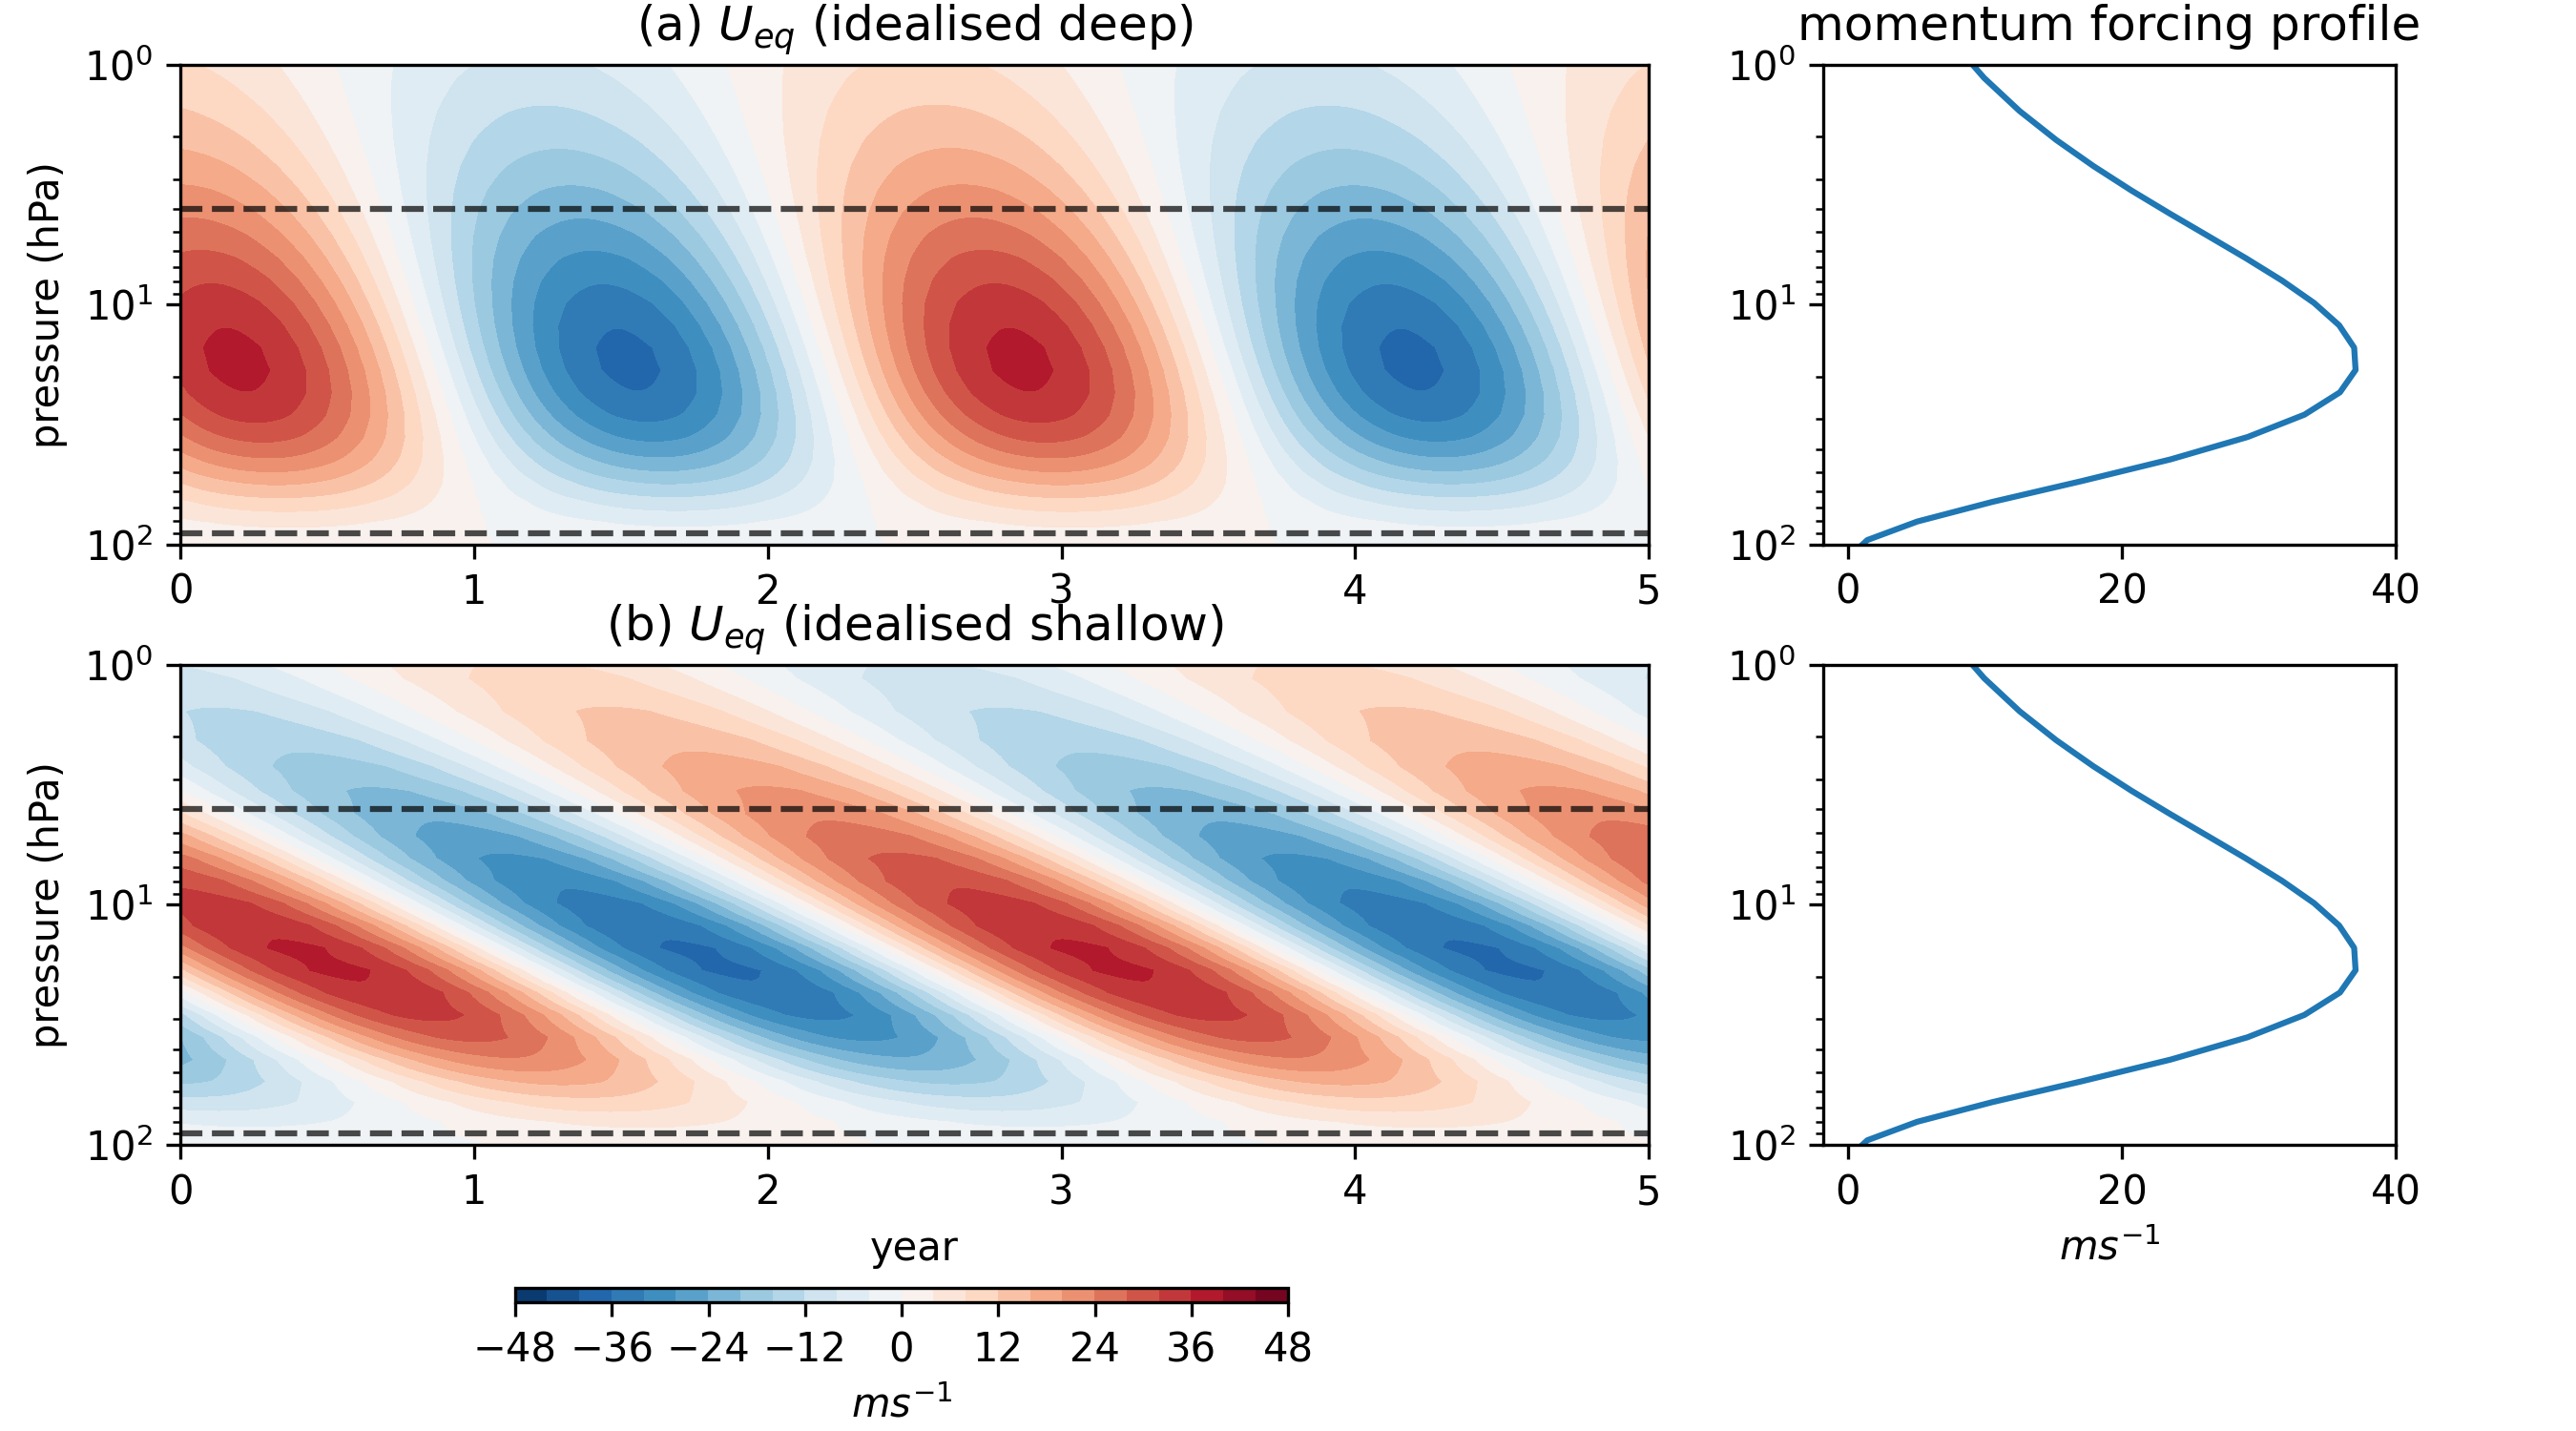
\includegraphics[width = \linewidth]{Figures/Figures-deepQBO/Idealised_QBO_features.png}
\caption[Idealised QBO winds used for nudging experiments]{Sample time-series of idealised equatorial ZMZW and associated momentum forcing profile for the deep (a and b respectively) and shallow (c and d respectively) QBO experiments. Horizontal dashed lines on (a) and (c) denote the 6 hPa and 90 hPa pressure levels between which we implement nudging towards the idealised wind in each experiment. Solid back lines denote the zero-wind line.}
\label{fig:Idealised_QBO_samples}
\end{center}
\end{figure}

%\begin{figure}[h!]
%\begin{center}
%\noindent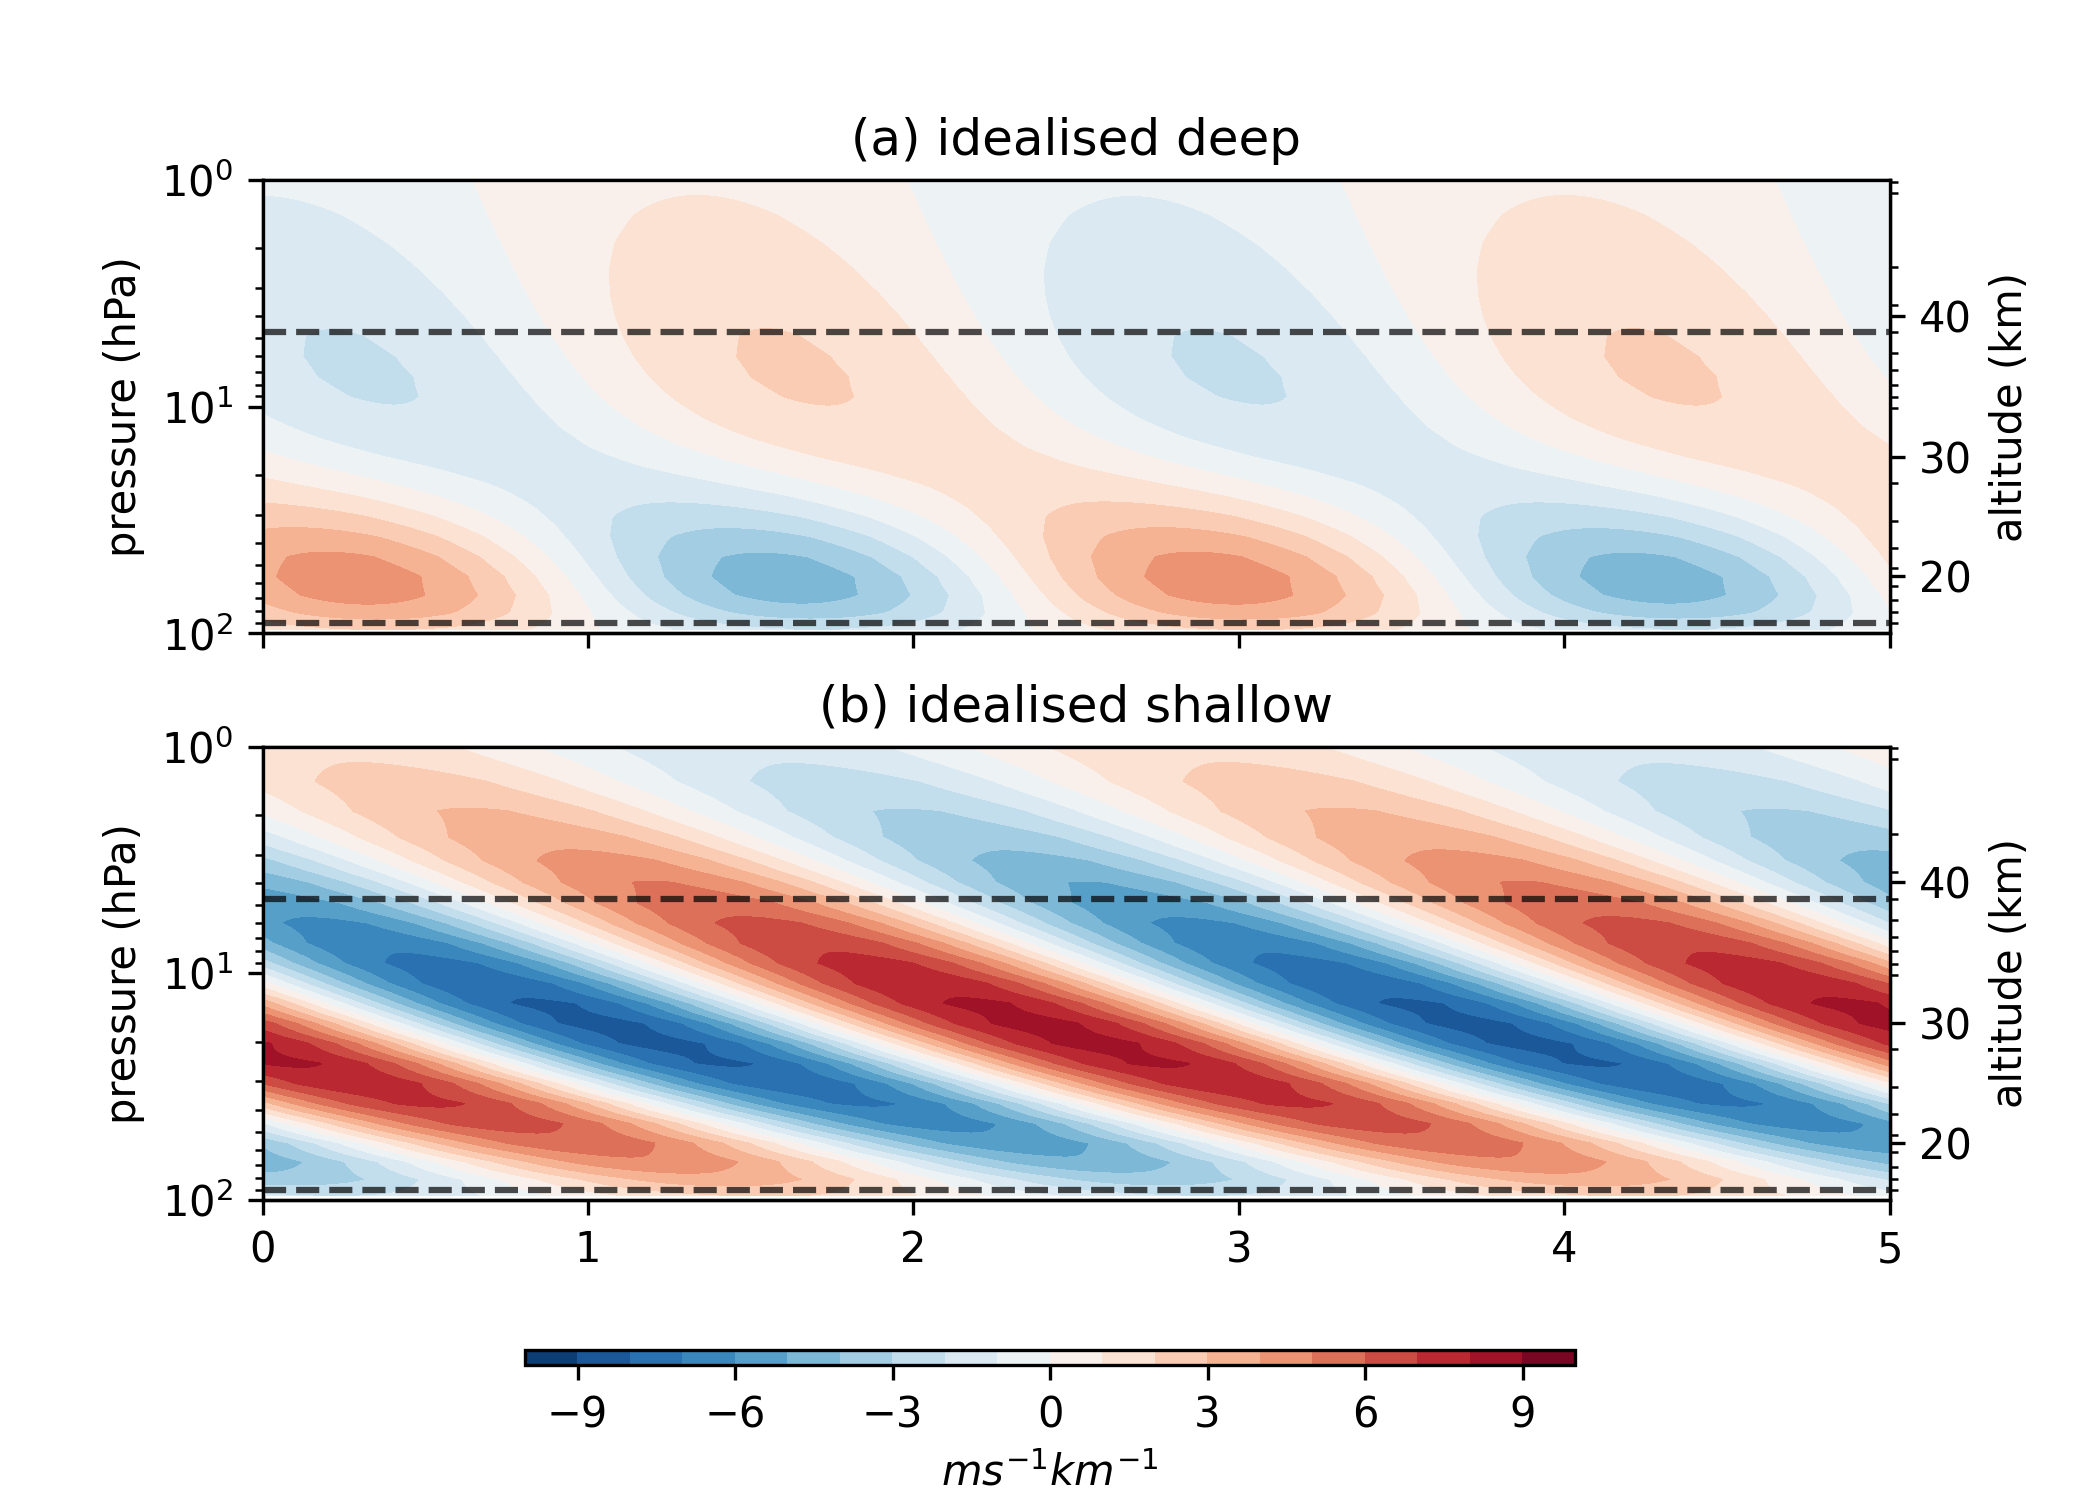
\includegraphics[width = 0.65\linewidth]{Figures/Figures-deepQBO/Idealised_QBO_descent_rates.png}
%\caption[Idealised QBO descent rates]{Sample time-series of descent rate in idealised equatorial ZMZW for the deep (\textbf{a}) and shallow (\textbf{b}) QBO experiments. The descent rates are defined as the 1st derivative of the QBO winds with respect to the vertical height coordinate, $z$ in $km$. Horizontal dashed lines denote the 6 hPa and 90 hPa pressure levels between which we implement nudging towards the idealised winds in each experiment.}
%\label{fig:Idealised_descent_rates}
%\end{center}
%\end{figure}

\section{QBO characteristics}
We first analyse the equatorial winds in each experiment and verify whether the implementation of nudging has resulted in the desired equatorial ZMZW profiles. Figures \ref{fig:experiment_QBOs}a and c show a 5 year sample of the equatorial winds in each experiment that results from implementing QBO nudging between the 90 hPa and 6 hPa levels. These winds reflect many of the key features of the idealised winds (figure \ref{fig:Idealised_QBO_samples}); the deep experiment exhibits vertical coherence in the middle stratosphere while the shallow simulation shows opposite phases of the QBO in the upper and lower sections of the nudging region (9 hPa-6 hPa). The period of ZMZW variations in both experiments is indicated by the Fourier power spectra shown in figures \ref{fig:experiment_QBOs}b and d. The mid-stratospheric winds ($\sim$90-10 hPa) exhibits peak Fourier power corresponding to a period close to the value specified by the idealised winds (32 months) in both experiments. The QBO variations produced by the nudging experiments also show good agreement in phase amplitude and period with that of the pi-clim cntrl (figures \ref{fig:experiment_QBOs}e and f). It also broadly resembles the winds in ERA-Interim (figures (\ref{fig:experiment_QBOs}g and h)) although the QBO from this dataset exhibits varying degrees of vertical coherence - a deep QBO phase is observed near month number 50 while a shallow QBO is evident near month number 15. These QBO samples confirm that the implementation of the nudging in our experiment has been effective in imposing different degrees of vertical coherence while retaining the characteristics of the QBOs in the un-nudged run and ERA-Interim.

\begin{figure}[h!]
\begin{center}
\noindent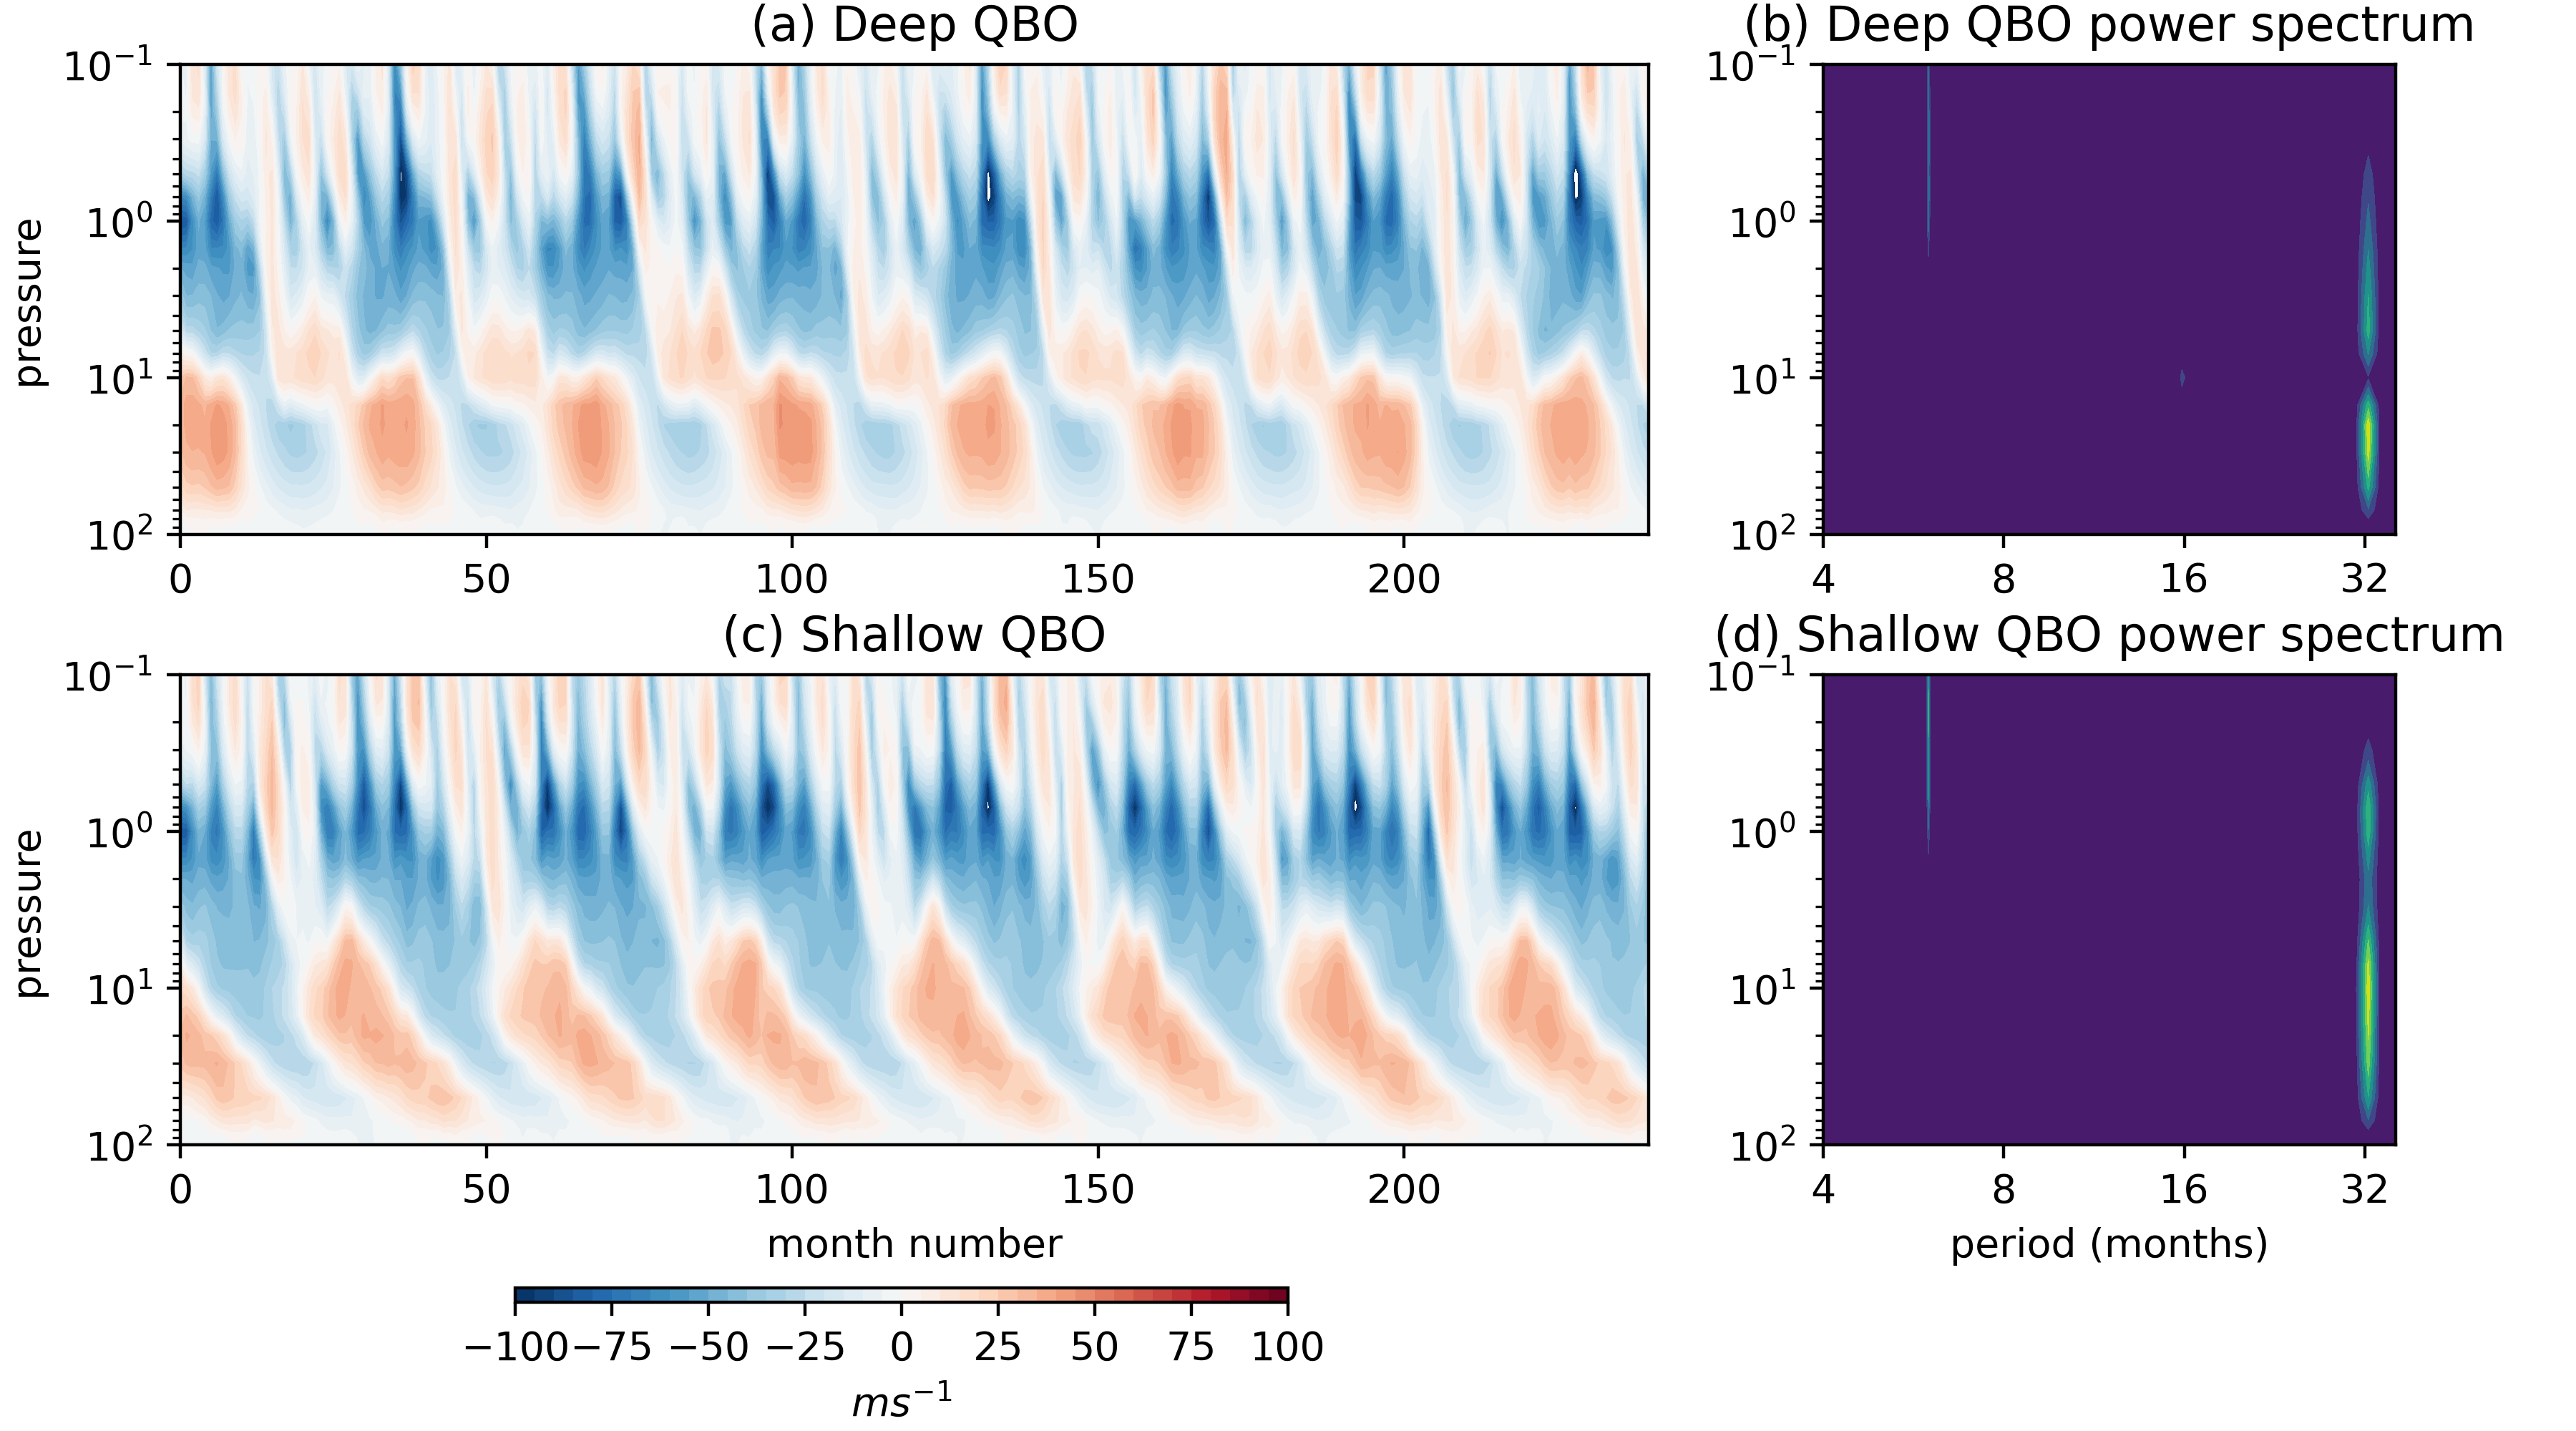
\includegraphics[width = \linewidth]{Figures/Figures-deepQBO/experiment_QBOs.png}
\caption[Equatorial ZMZW time-height profiles from QBO experiments]{5 year sample of ZMZW averaged between 5$^{\circ}$\,S--5$^{\circ}$\,N latitude from the deep QBO (a), shallow QBO (c) and pi-clim cntrl (e) simulations and ERA-Interim (g). Thick black contours denote the 0-wind line where westerlies meet easterlies. Sub-figures b, d, f and h show Fourier Power spectra for equatorial winds at various levels from the same datasets.}
\label{fig:experiment_QBOs}
\end{center}
\end{figure}

While the QBO of both simulations reflects some of the main characteristics of the target nudging winds, there is a notable asymmetry in the amplitudes of the two QBO phases in both experiments with the westerly phase amplitude appearing larger in all QBO cycles throughout each simulation. This is an unexpected result - we defined the target nudging field using equation \ref{eq:imposed_U} which ensures each phase of the idealised QBO exhibits identical magnitude (i.e. $F(p)$ in equation \ref{eq:imposed_U} is constant in time). To examine this asymmetry further, we analyse the timeseries of simulated (model output) and idealised (nudging input) winds on individual pressure levels (Figures \ref{fig:winds_on_levs_deep} and \ref{fig:winds_on_levs_shallow}). In the deep experiment (figure \ref{fig:winds_on_levs_deep}), the easterly phase of the QBO is in good agreement (within $\sim$1\%) with the idealised winds on each of the pressure levels sampled. In contrast, the magnitude of the westerly phase resulting from the simulation systematically 'over-shoots' compared to the nudging winds. This effect is apparent throughout much of the mid-stratosphere (10 hPa-50 hPa) and suggests the possibility of a westerly momentum forcing term in the model which acts to override the influence of the nudging scheme. This in turn may suggest that our selection of nudging timescale, $\tau$ = 6 hours, is too long in relation to timescales over which other forcing terms act. The effect is less pronounced in the shallow experiment with only the QBO at 50 hPa exhibiting notable over-representation in westerly amplitude. The source of additional forcing term is unclear but is likely closely associated with Kelvin or gravity wave forcing as this is the primary source of the westerly QBO phase (see section \ref{sec:equatorial_strat}). This may indicate the requirement for a shorter nudging timescale for future nudged QBO experiments using this configuration as the model appears insufficiently constrained at the positive extremes of the QBO. This is a surprising result; \cite{telfordTechnical2008} present an evaluation of the efficacy of the MetOffice Unified Model (of which our simulations are a member) nudging scheme and show that, using $\tau = 6$ hours, zonal winds in the mid-stratosphere can be nudged towards reanalysis fields with a high degree of correlation ($r>0.98$) between model output and target winds. Further work beyond the scope of this study is required to establish the source of this discrepancy but \cite{telfordTechnical2008} points out that the primary reason for the choice of $\tau = 6$ hours is due to the time resolution of the reanalysis data as opposed to necessarily due to model instability. In our experiments, the time resolution of the nudging fields are not constrained by data availability as they are synthetically generated and, as a result, experiments with a smaller $\tau$ are feasible and may rectify the biases evident from figures \ref{fig:winds_on_levs_deep} and \ref{fig:winds_on_levs_shallow}.

\begin{figure}[h!]
\begin{center}
\noindent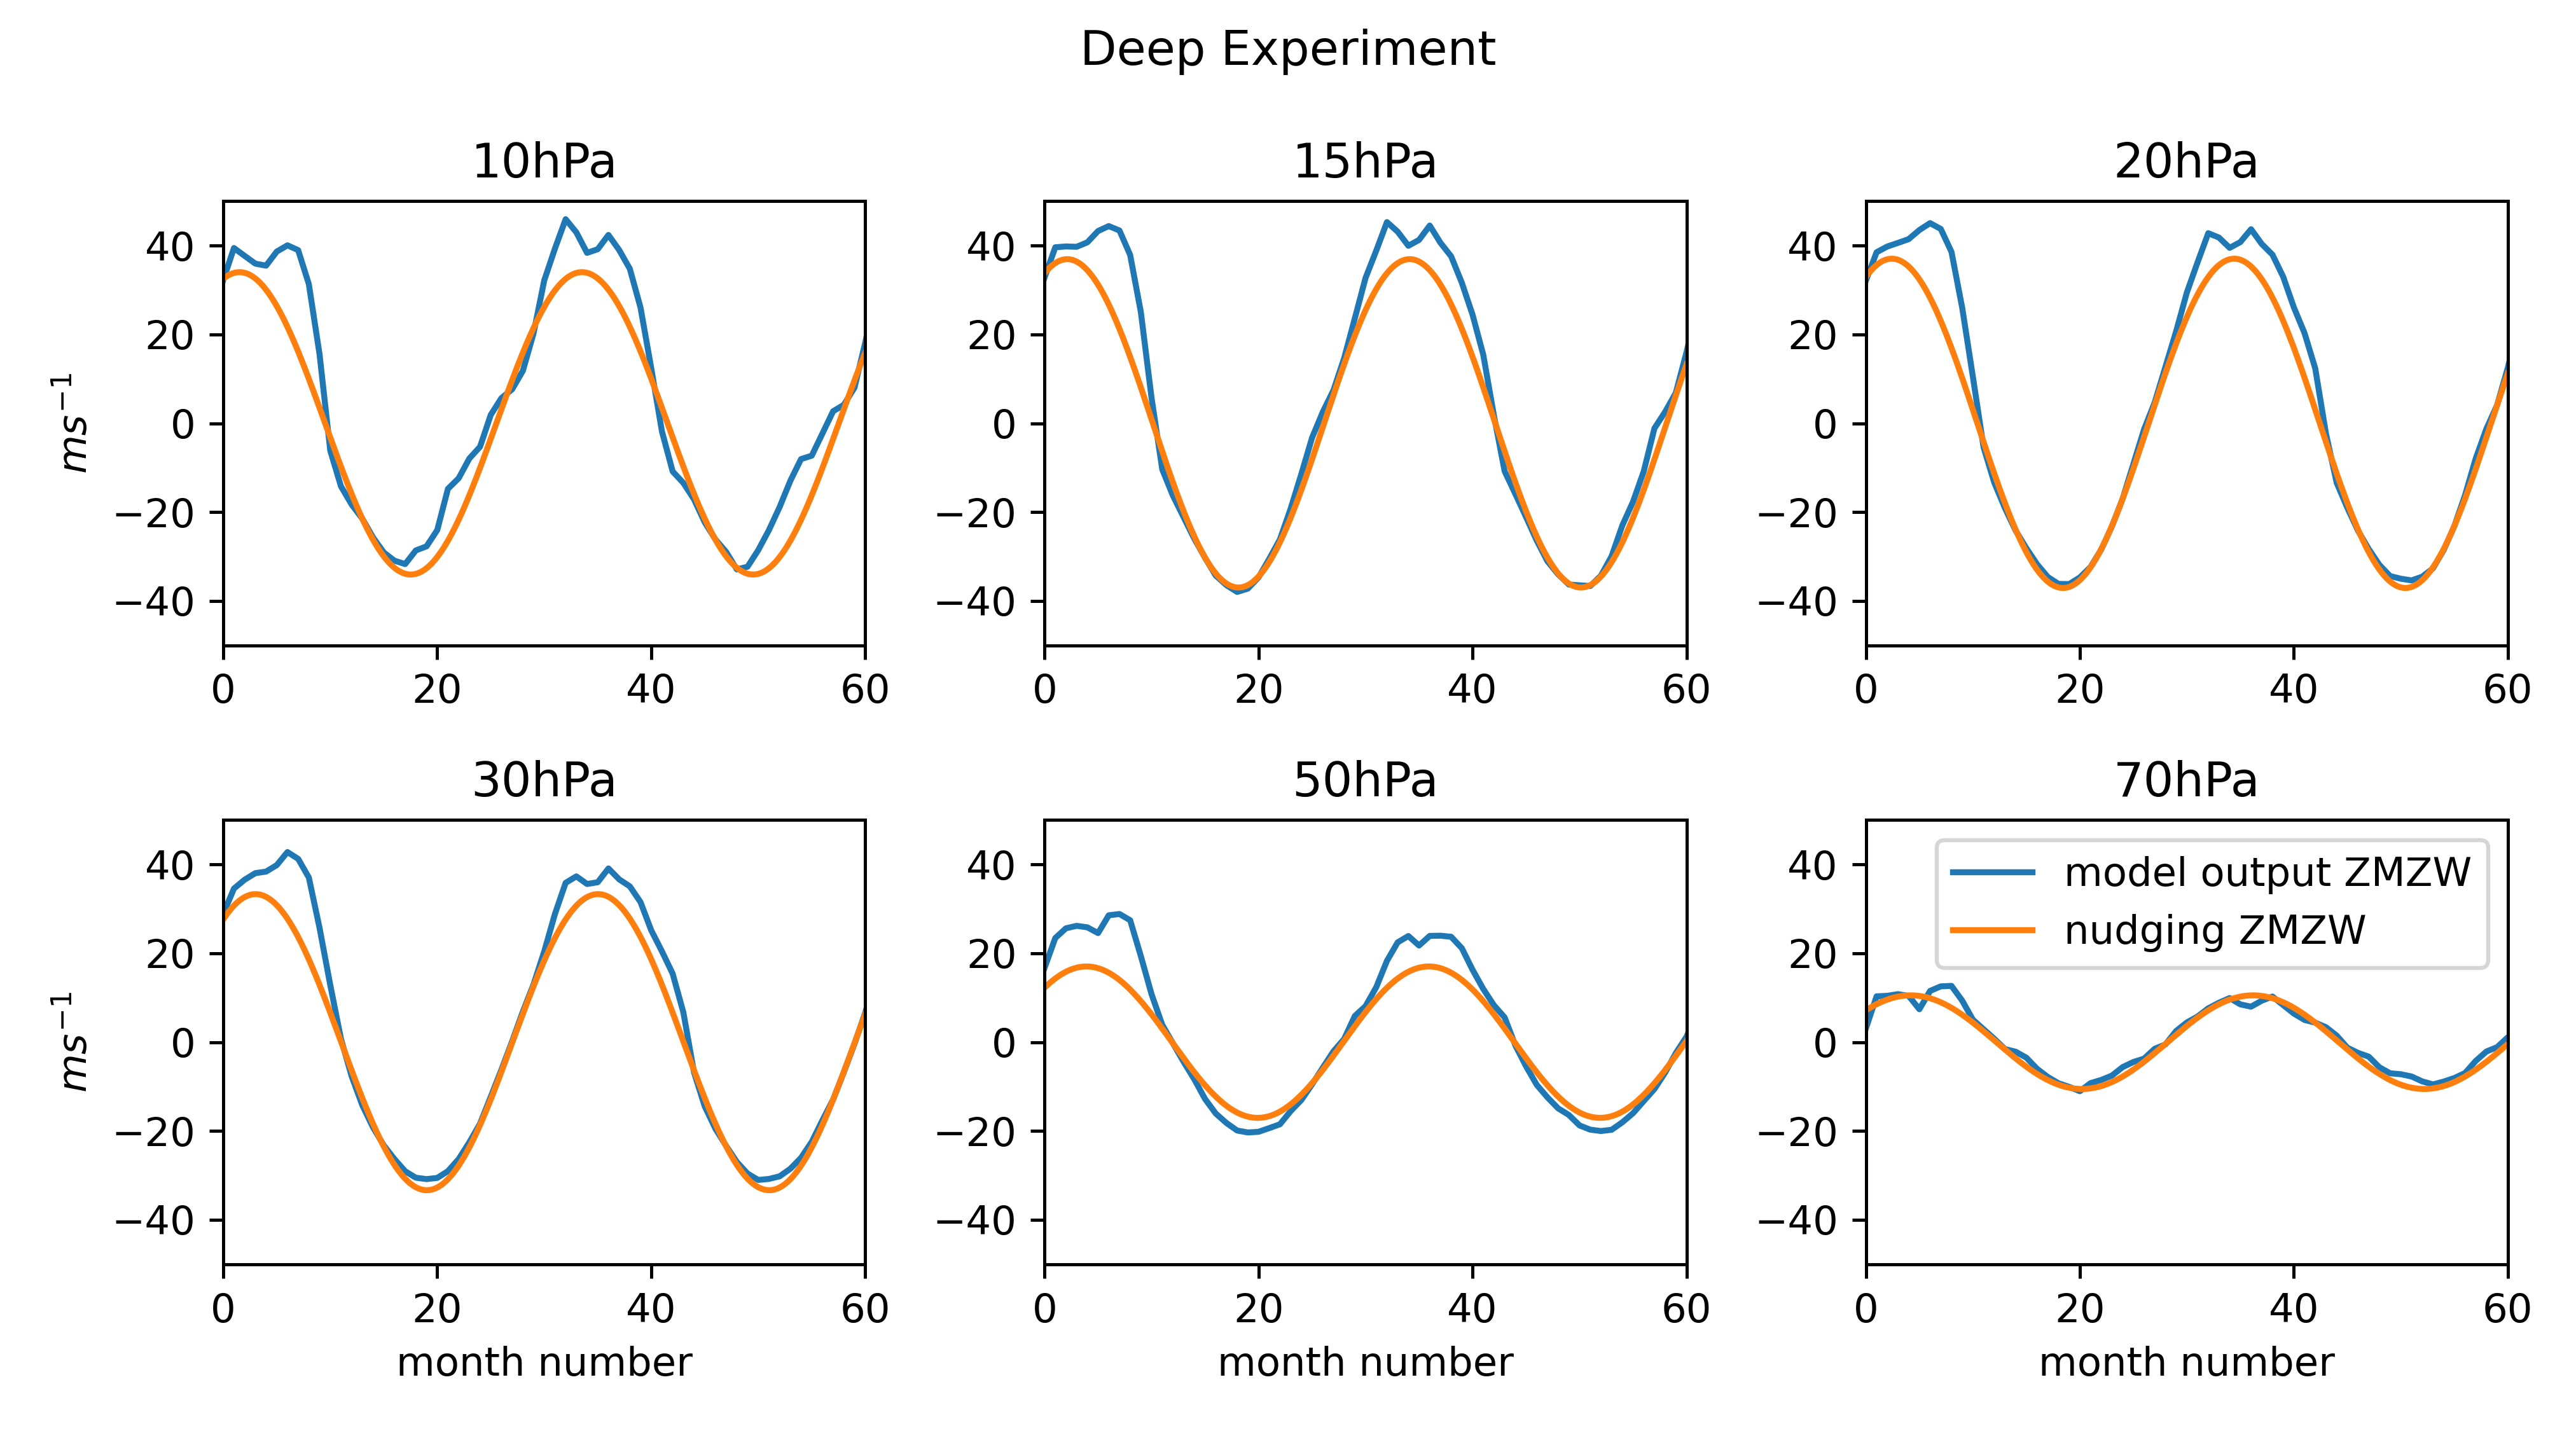
\includegraphics[width = 0.95\linewidth]{Figures/Figures-deepQBO/winds_on_lev_nudging_deep.png}
\caption[Equatorial ZMZW on individual pressure levels in the deep QBO experiment]{5 year sample of ZMZW on individual pressure levels averaged between 5$^{\circ}$\,S--5$^{\circ}$\,N latitude from the deep QBO experiments (blue) and the Idealised wind field used for nudging in the same experiment (orange).}
\label{fig:winds_on_levs_deep}
\end{center}
\end{figure}

\begin{figure}[h!]
\begin{center}
\noindent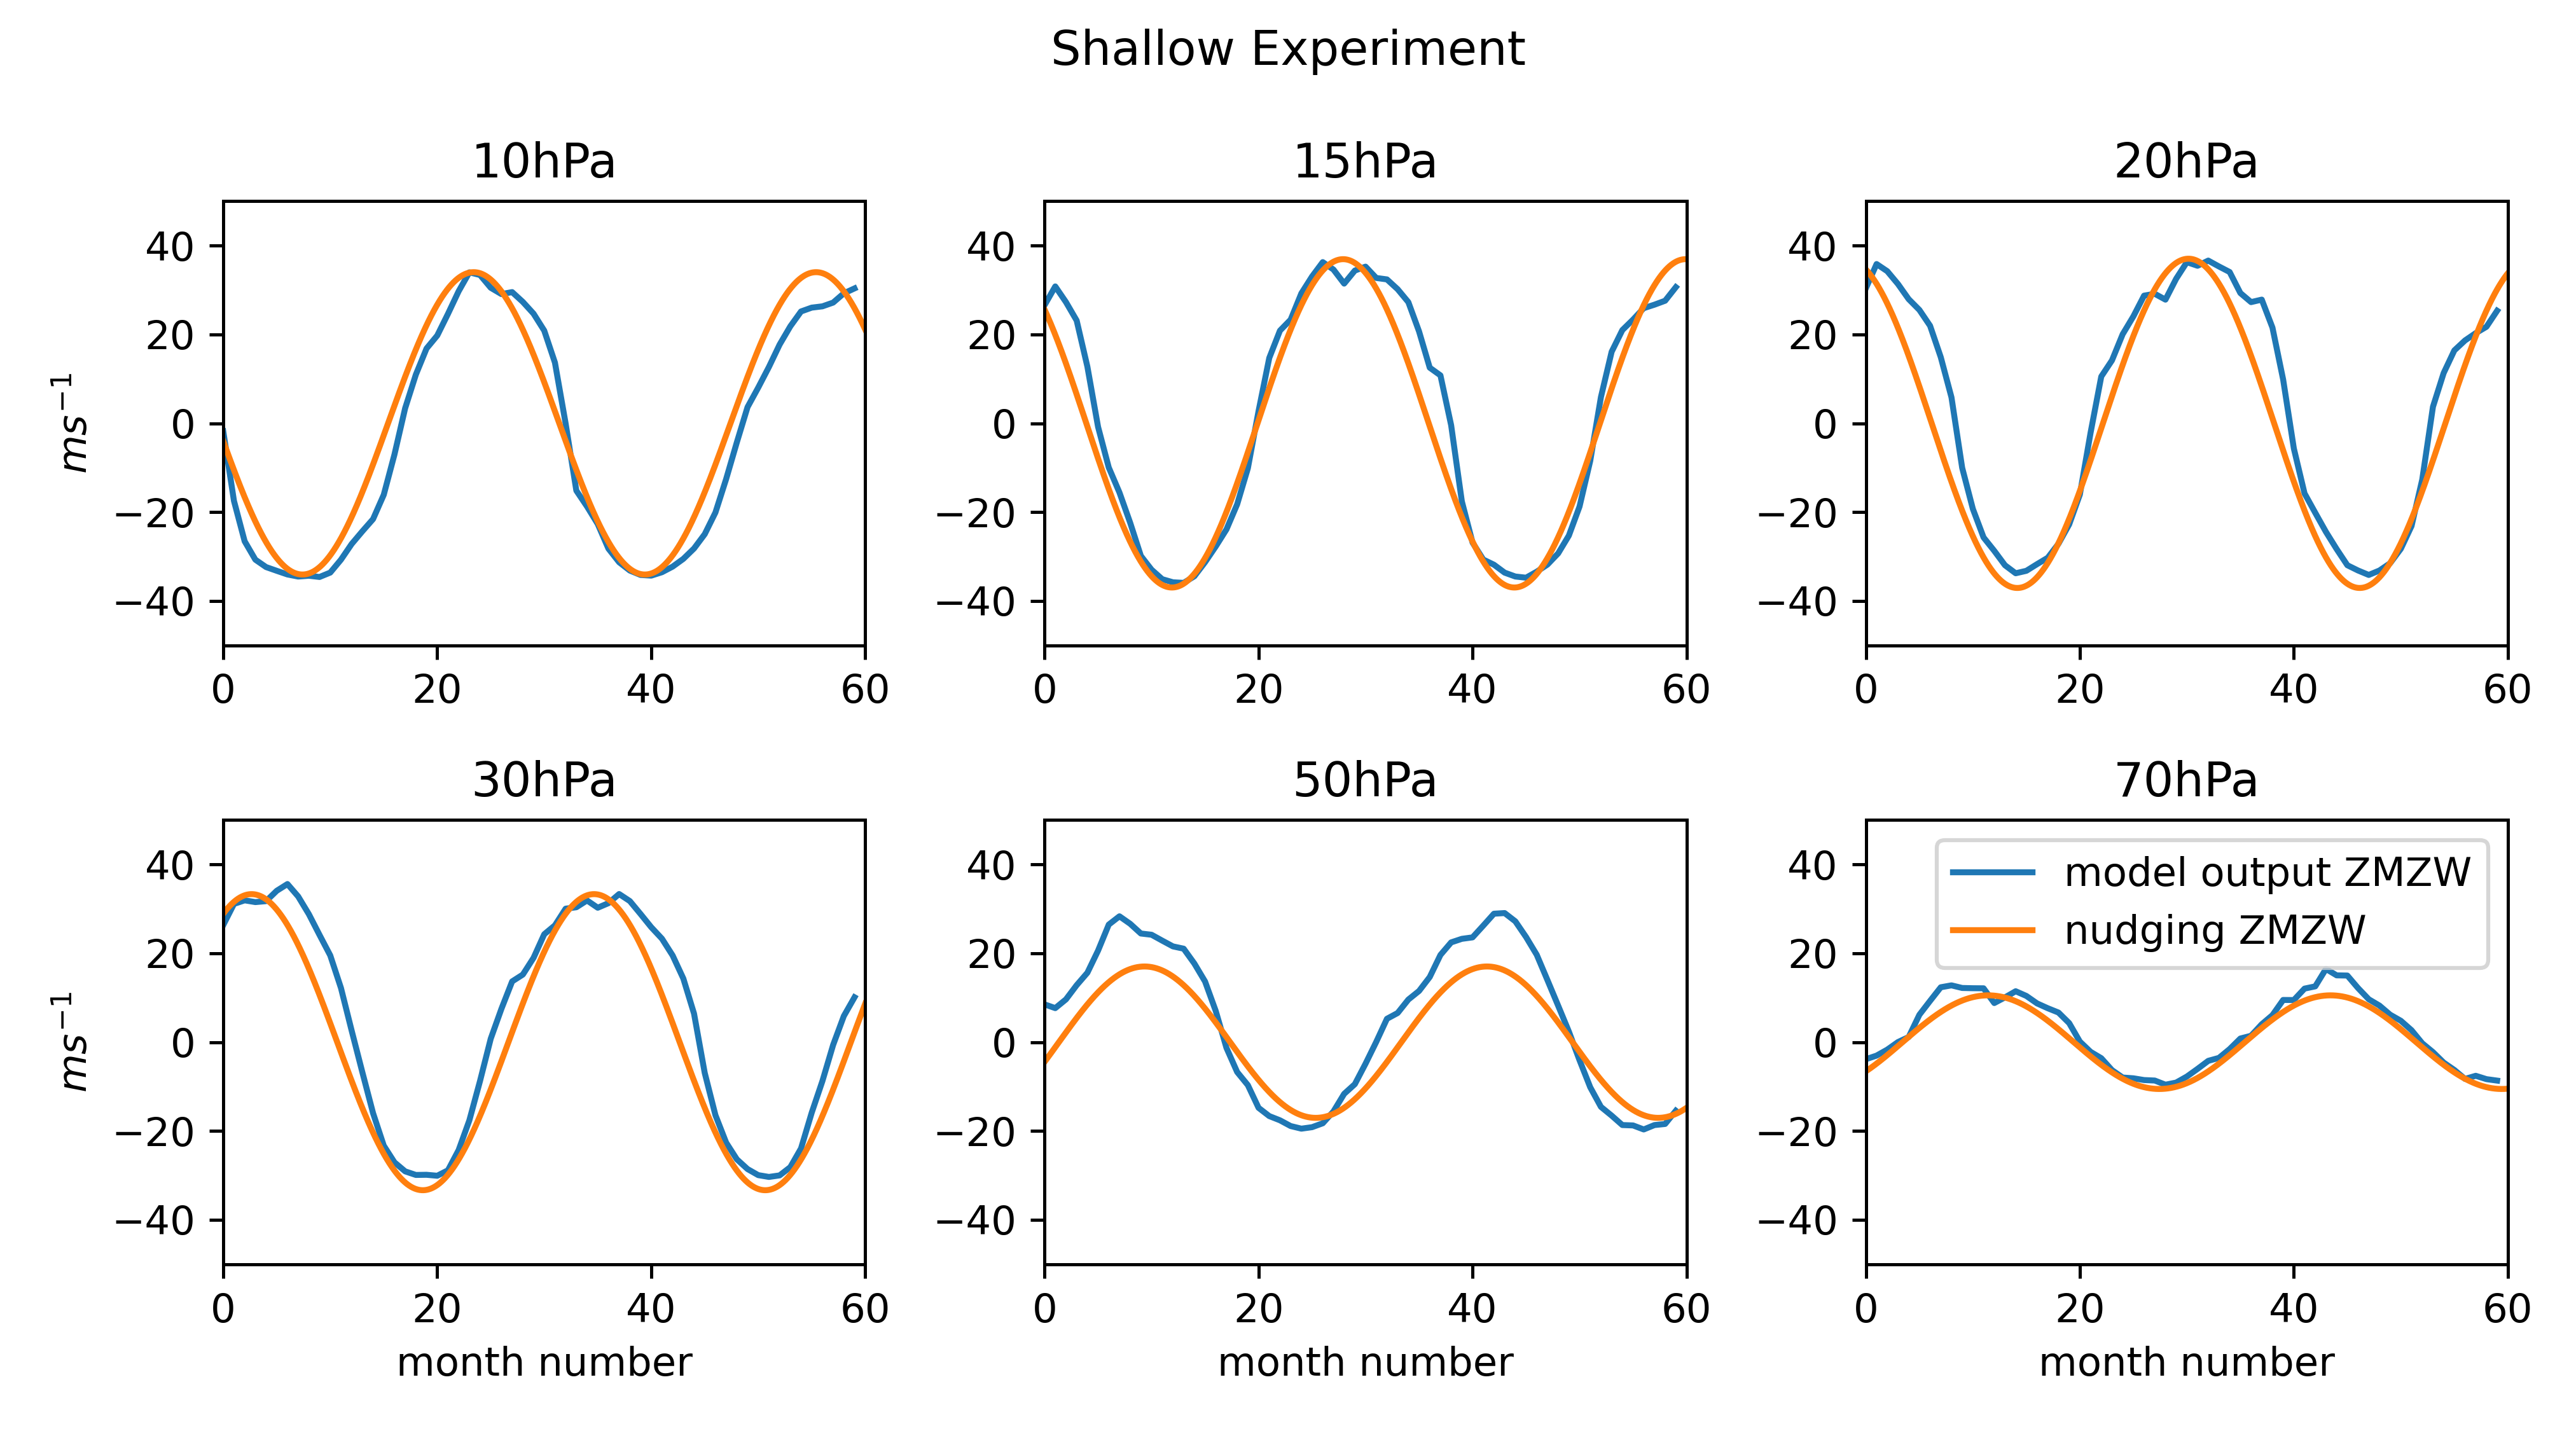
\includegraphics[width = 0.95\linewidth]{Figures/Figures-deepQBO/winds_on_lev_nudging_shallow.png}
\caption[Equatorial ZMZW on individual pressure levels in the shallow QBO experiment]{Like figure \ref{fig:winds_on_levs_deep} for the shallow QBO experiment.}
\label{fig:winds_on_levs_shallow}
\end{center}
\end{figure}

While this bias does lead to marginal asymmetries in QBO phases, the desired vertical structures is still obtained in both experiments which is the focus of this study and therefore we proceed with the simulations for analysis of QBO teleconnections in the next section. The possible detrimental effect of this amplitude bias is that NH winters may preferentially occur under one QBO phase more than the other if we define a QBO phase using equatorial winds over a given threshold (5$ms^{-1}$ is commonly used). As a result, in all analysis of these simulations we note the number of NH winters exhibiting each QBO phase and only draw major conclusions in cases where their abundance is broadly comparable. 

\section{Other atmospheric characteristics}

In addition to the imposed QBO states, both experiments also exhibit variations in ZMZW on the 1 hPa level and above corresponding to a period of $\sim$6 months which indicates the presence of an SAO like variation (see figure \ref{fig:experiment_QBOs}). Previous work suggests a key role for this region in equator-vortex teleconnections (e.g. \cite{grayForecasting2020a}) as well as elements of synchronisation between the QBO and SAO \citep{kuaiNonstationary2009c}. As each experiment imposes significantly different QBO states, features of SAO in the experiments may play a key role in dictating responses from the vortex, troposphere and surface.

SAO differences can be formally diagnosed by analysing the climatological seasonal cycle in equatorial winds (figure \ref{fig:experiment_SAOs}, note that the pressure level scale in this figure starts at 10 hPa while that of figure \ref{fig:experiment_QBOs} starts at 100 hPa). This indicates the mean state of each simulation's SAO; the westerly phase of the SAO appearing in early NH winter (Sep-Nov), which is attributed to the dissipation of Kelvin waves and small scale inertia-gravity waves \citep{dunkertonRole1979, hitchmanEstimation1988}, is significantly weaker and exhibits less vertical extent in the deep experiment compared to the shallow - difference plots of the nudged experiments' seasonal cycles (figure \ref{fig:experiment_SAOs}c) show significant differences in Sep-Oct near the 0.1 hPa level. The timing of phase transitions from westerly to easterly in early NH winter (denoted by the climatological zero wind line on approximately the 0.1 hPa level) is also marginally later in the shallow experiment. These differences in the extent of the westerly SAO phase could play a key role in equator-vortex interactions in each experiment as these features, particularly phase transition timings, have been shown to associate with the timing of SSWs \citep{grayData2001, hamiltonEffects1998}. The largest differences between the experiment SAOs are evident in the magnitude of the easterly phase, driven by summer hemisphere easterly meridional advection by the BDC, in mid-late NH winter (Jan-Mar) near the 1 hPa level. Here, the shallow experiment's easterlies are significantly larger however easterly phases in both experiments are stronger than those in the pi-clim cntrl (figure \ref{fig:experiment_SAOs}C). While these differences highlight the potential impact that the degree of vertical coherence in the QBO may have have on the SAO, the role these variations play in teleconnections with the vortex in each experiment is less clear and explored further in sections \ref{sec:vortex_responses_QBO} and \ref{sec:role_SAO}.

\begin{figure}[h!]
\begin{center}
\noindent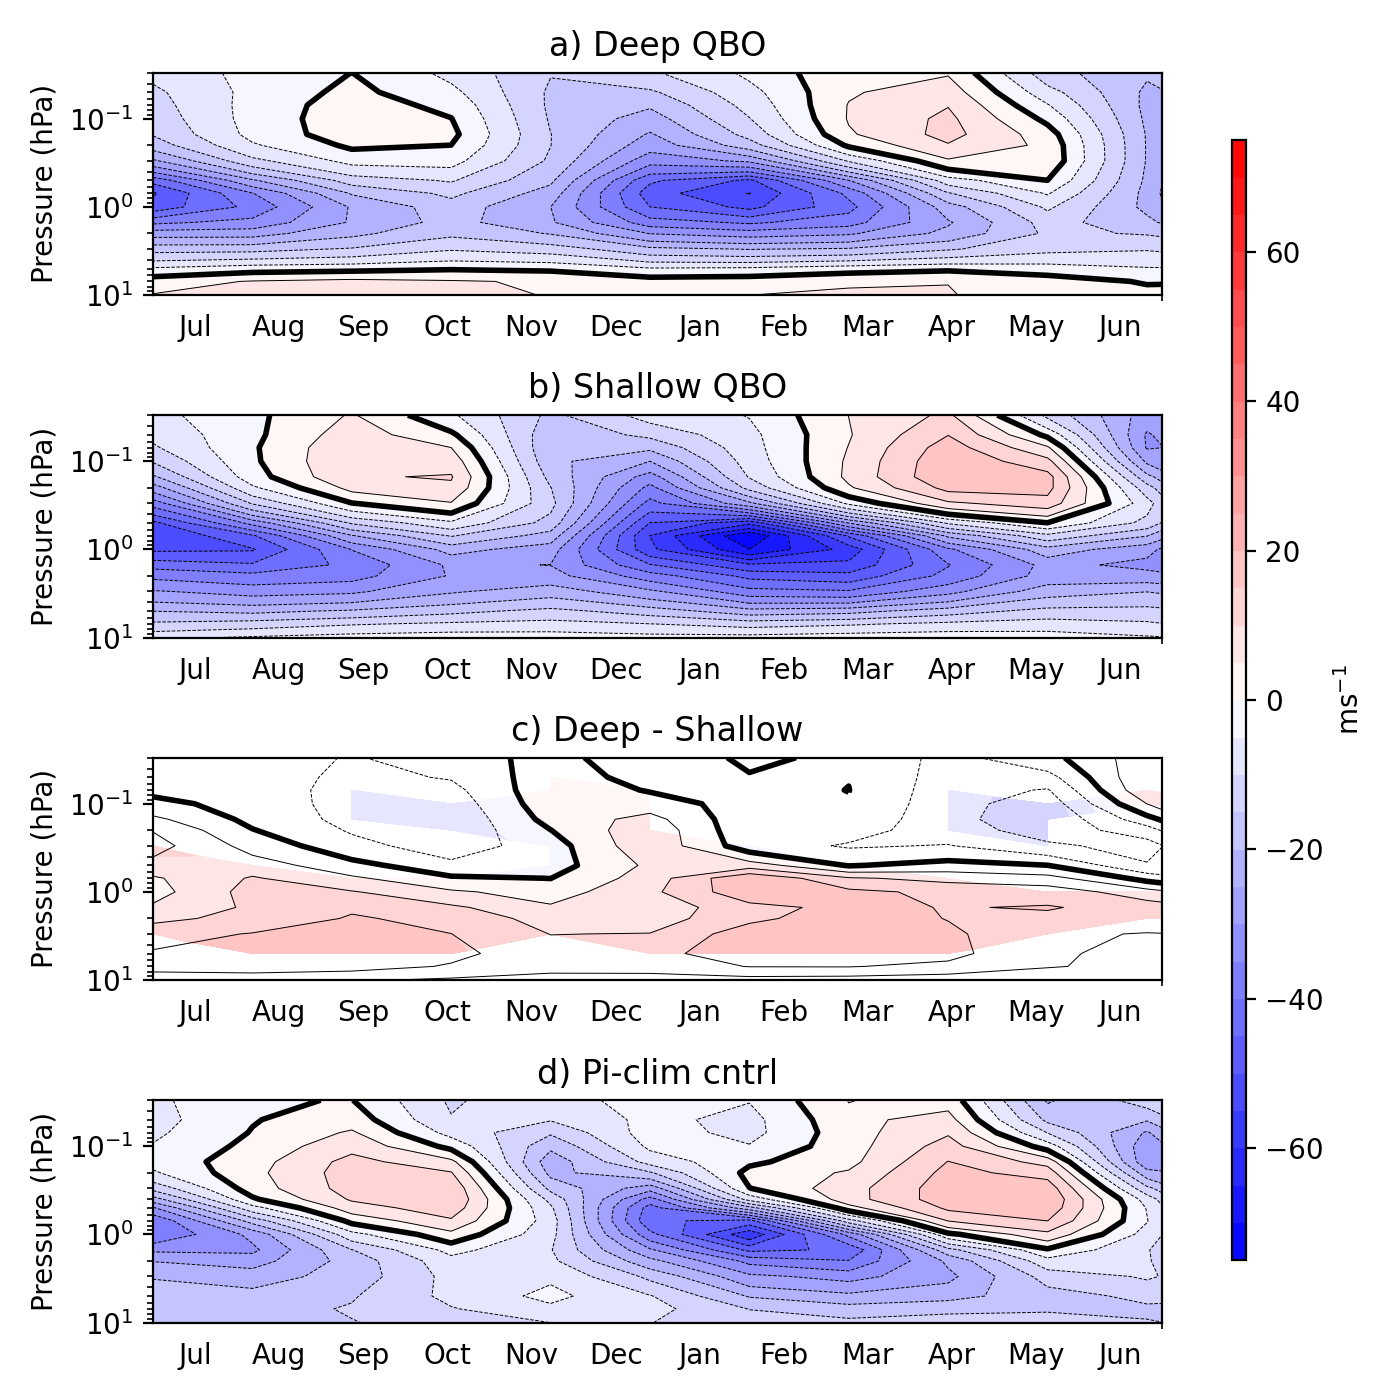
\includegraphics[width = 0.75\linewidth]{Figures/Figures-deepQBO/SAO_seasonal_cycles.png}
\caption[Climatological seasonal cycle of the SAO in QBO experiments]{Climatological seasonal cycle of ZMZW averaged between 5$^{\circ}$\,S--5$^{\circ}$\,N latitude from the deep (a) and shallow (b) QBO experiments. Panel c shows climatological differences between deep and shallow seasonal cycles and the cycle from the pi-clim cntrl is provided in panel d. Coloured shading on difference panel c denote differences significant to the 95\% level under a 2-tailed student's t-test.}
\label{fig:experiment_SAOs}
\end{center}
\end{figure}

Another key mode of variation we consider in each experiment is the vortex and the frequency of SSWs. Figure \ref{fig:SSW_histogram_experiments} shows the average NH winter season SSW rates in each experiment. Over the whole winter season (figure \ref{fig:SSW_histogram_experiments}a), each experiment exhibits an SSW rate which lies within 1 standard error of each other as well as the rate exhibited by ERA-Interim (red bars). The deep experiment shows the most SSWs (0.61 events per winter) however the differences between each SSW rate are not deemed significant to the 95\% level using the bootstrap and parametric significance test outlined in section \ref{sec:stat_methods}. 

\begin{figure}[h!]
\begin{center}
\noindent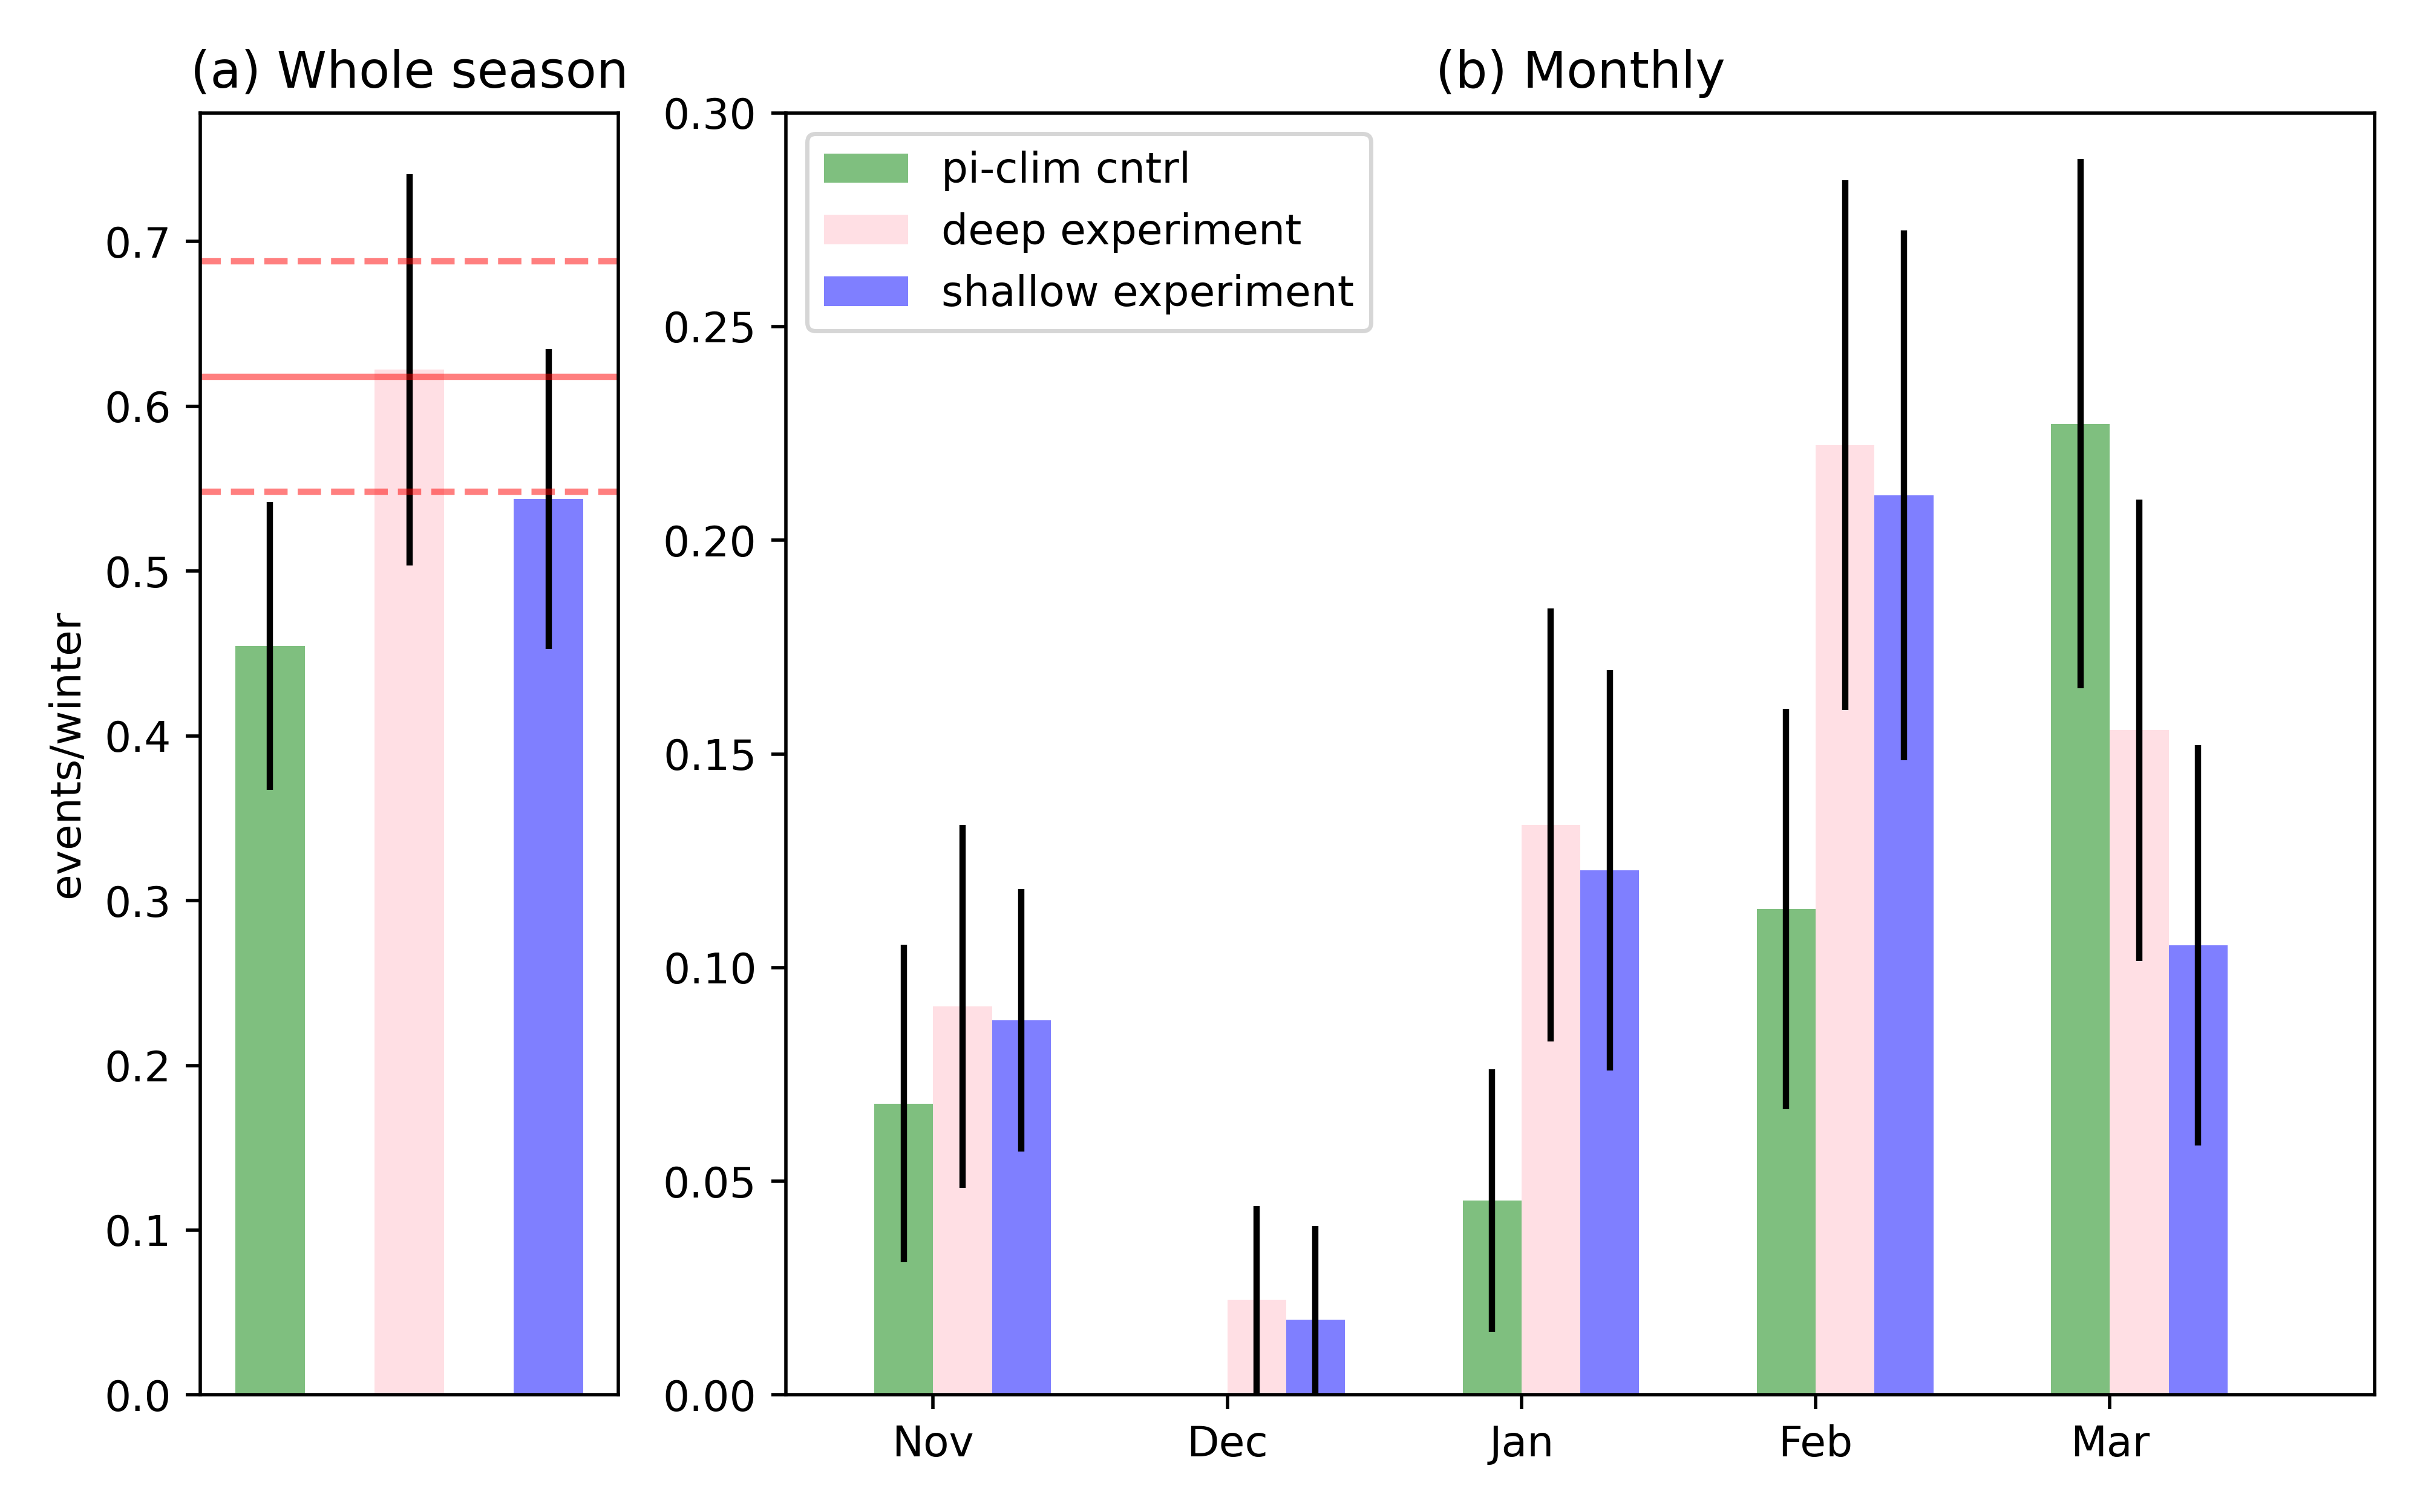
\includegraphics[width = 0.8\linewidth]{Figures/Figures-deepQBO/SSW_hist.png}
\caption[SSWs per NH winter season in QBO experiments]{\textbf{a}: SSWs per NH winter season (Nov-Mar) in the deep QBO, shallow QBO and pi-clim cntrl simulations. \textbf{b}: SSW rates separated by months. Error bars on (a) and (b) signify the standard error on rates calculated as $\frac{\sigma}{\sqrt{N}}$ where $\sigma$ is the standard deviation of the SSW per winter timeseries and $N$ is the number of years in the simulation. SSW rates from ERA-Interim are also included for comparison.}
\label{fig:SSW_histogram_experiments}
\end{center}
\end{figure}

We also analyse the seasonal distribution of SSWs (figure \ref{fig:SSW_histogram_experiments}b). Each simulation shows a significant overestimation in November SSWs, a similar effect to that shown in the pi-control and discussed in section \ref{sec:strat_var_UKESM} (see figure \ref{fig:SSW_histogram}). This November SSW bias is similar across all simulations and may influence the vortex in mid-late winter as it recovers from a disruption in November which precludes significant planetary wave driving. This effect is evident in the December SSW rates for all simulations which is marginally lower than in ERA-Interim. How these November and December rates may interact with QBO teleconnections is unclear however, their influence may be non-negligible; potential signals from the QBO in mid-late winter may be obscured if the vortex of each experiment tends to be disrupted unrealistically early in the winter. As a result in all diagnostics in the following sections, sensitivity tests were performed to assess whether removing years which contain November SSWs significantly changed the response patterns. Over the remainder of the winter season (Jan-Mar), the pi-clim cntrl exhibits steadily increasing SSW rates between mid and late winter. Introducing both a perpetually deep and shallow QBO in the nudged experiments appears to recover the seasonal distribution exhibited by ERA-Interim, increasing rates between Dec-Feb followed by a decrease in Mar. The reason for this is unclear and may point to significant late winter interactions between the QBO and the vortex in these simulations which are examined in closer detail in section \ref{sec:vortex_responses_QBO}.

\section{Surface responses to deep and shallow QBOs}
\label{sec:MSLP_responses}
So far, we have shown that both nudged experiments exhibit the desired vertical structure in the QBO as well as realistic variations in the SAO and the vortex. The focus of this study however, is the different teleconnections that arise between the equatorial stratosphere and other parts of the climate system. In particular, we focus on the key finding of \cite{andrewsObserved2019d}; that the NAO and AO response to the QBO is enhanced when the QBO exhibits a higher degree of vertical coherence. 

To test this phenomenon explicitly, we analyse diagnostics of surface variability (specifically MSLP) under different QBO conditions in each simulation to compare the nature of teleconnections in each case. First, we examine whether the un-nudged simulation (the pi-clim cntrl) exhibits connection between the QBO and the surface. Figure \ref{fig:SLP_piclim} shows composites of NH MSLP associated with different QBO phases (top two rows) as well as the composite difference (QBOE - QBOW, bottom row) from the pi-clim cntrl. The QBO phase is defined using early winter (Nov-Dec) equatorial winds on the 50 hPa level, a standard level used in previous studies \citep{ansteyHighlatitude2014b} and located in the middle of the nudging region for both relaxed experiments (we analyse the variation of results with QBO height in the following sections). There are marginally more occurrences of early winter QBOW phases in each month (parentheses in figure \ref{fig:SLP_piclim}, top 2 rows) indicating a degree of locking of the QBO to the seasonal cycle, an effect discussed by \cite{rajendranSynchronisation2016b}. However, the abundance of each phase is comparable enough to carry out composite analysis.

\begin{figure}[h!]
\begin{center}
\noindent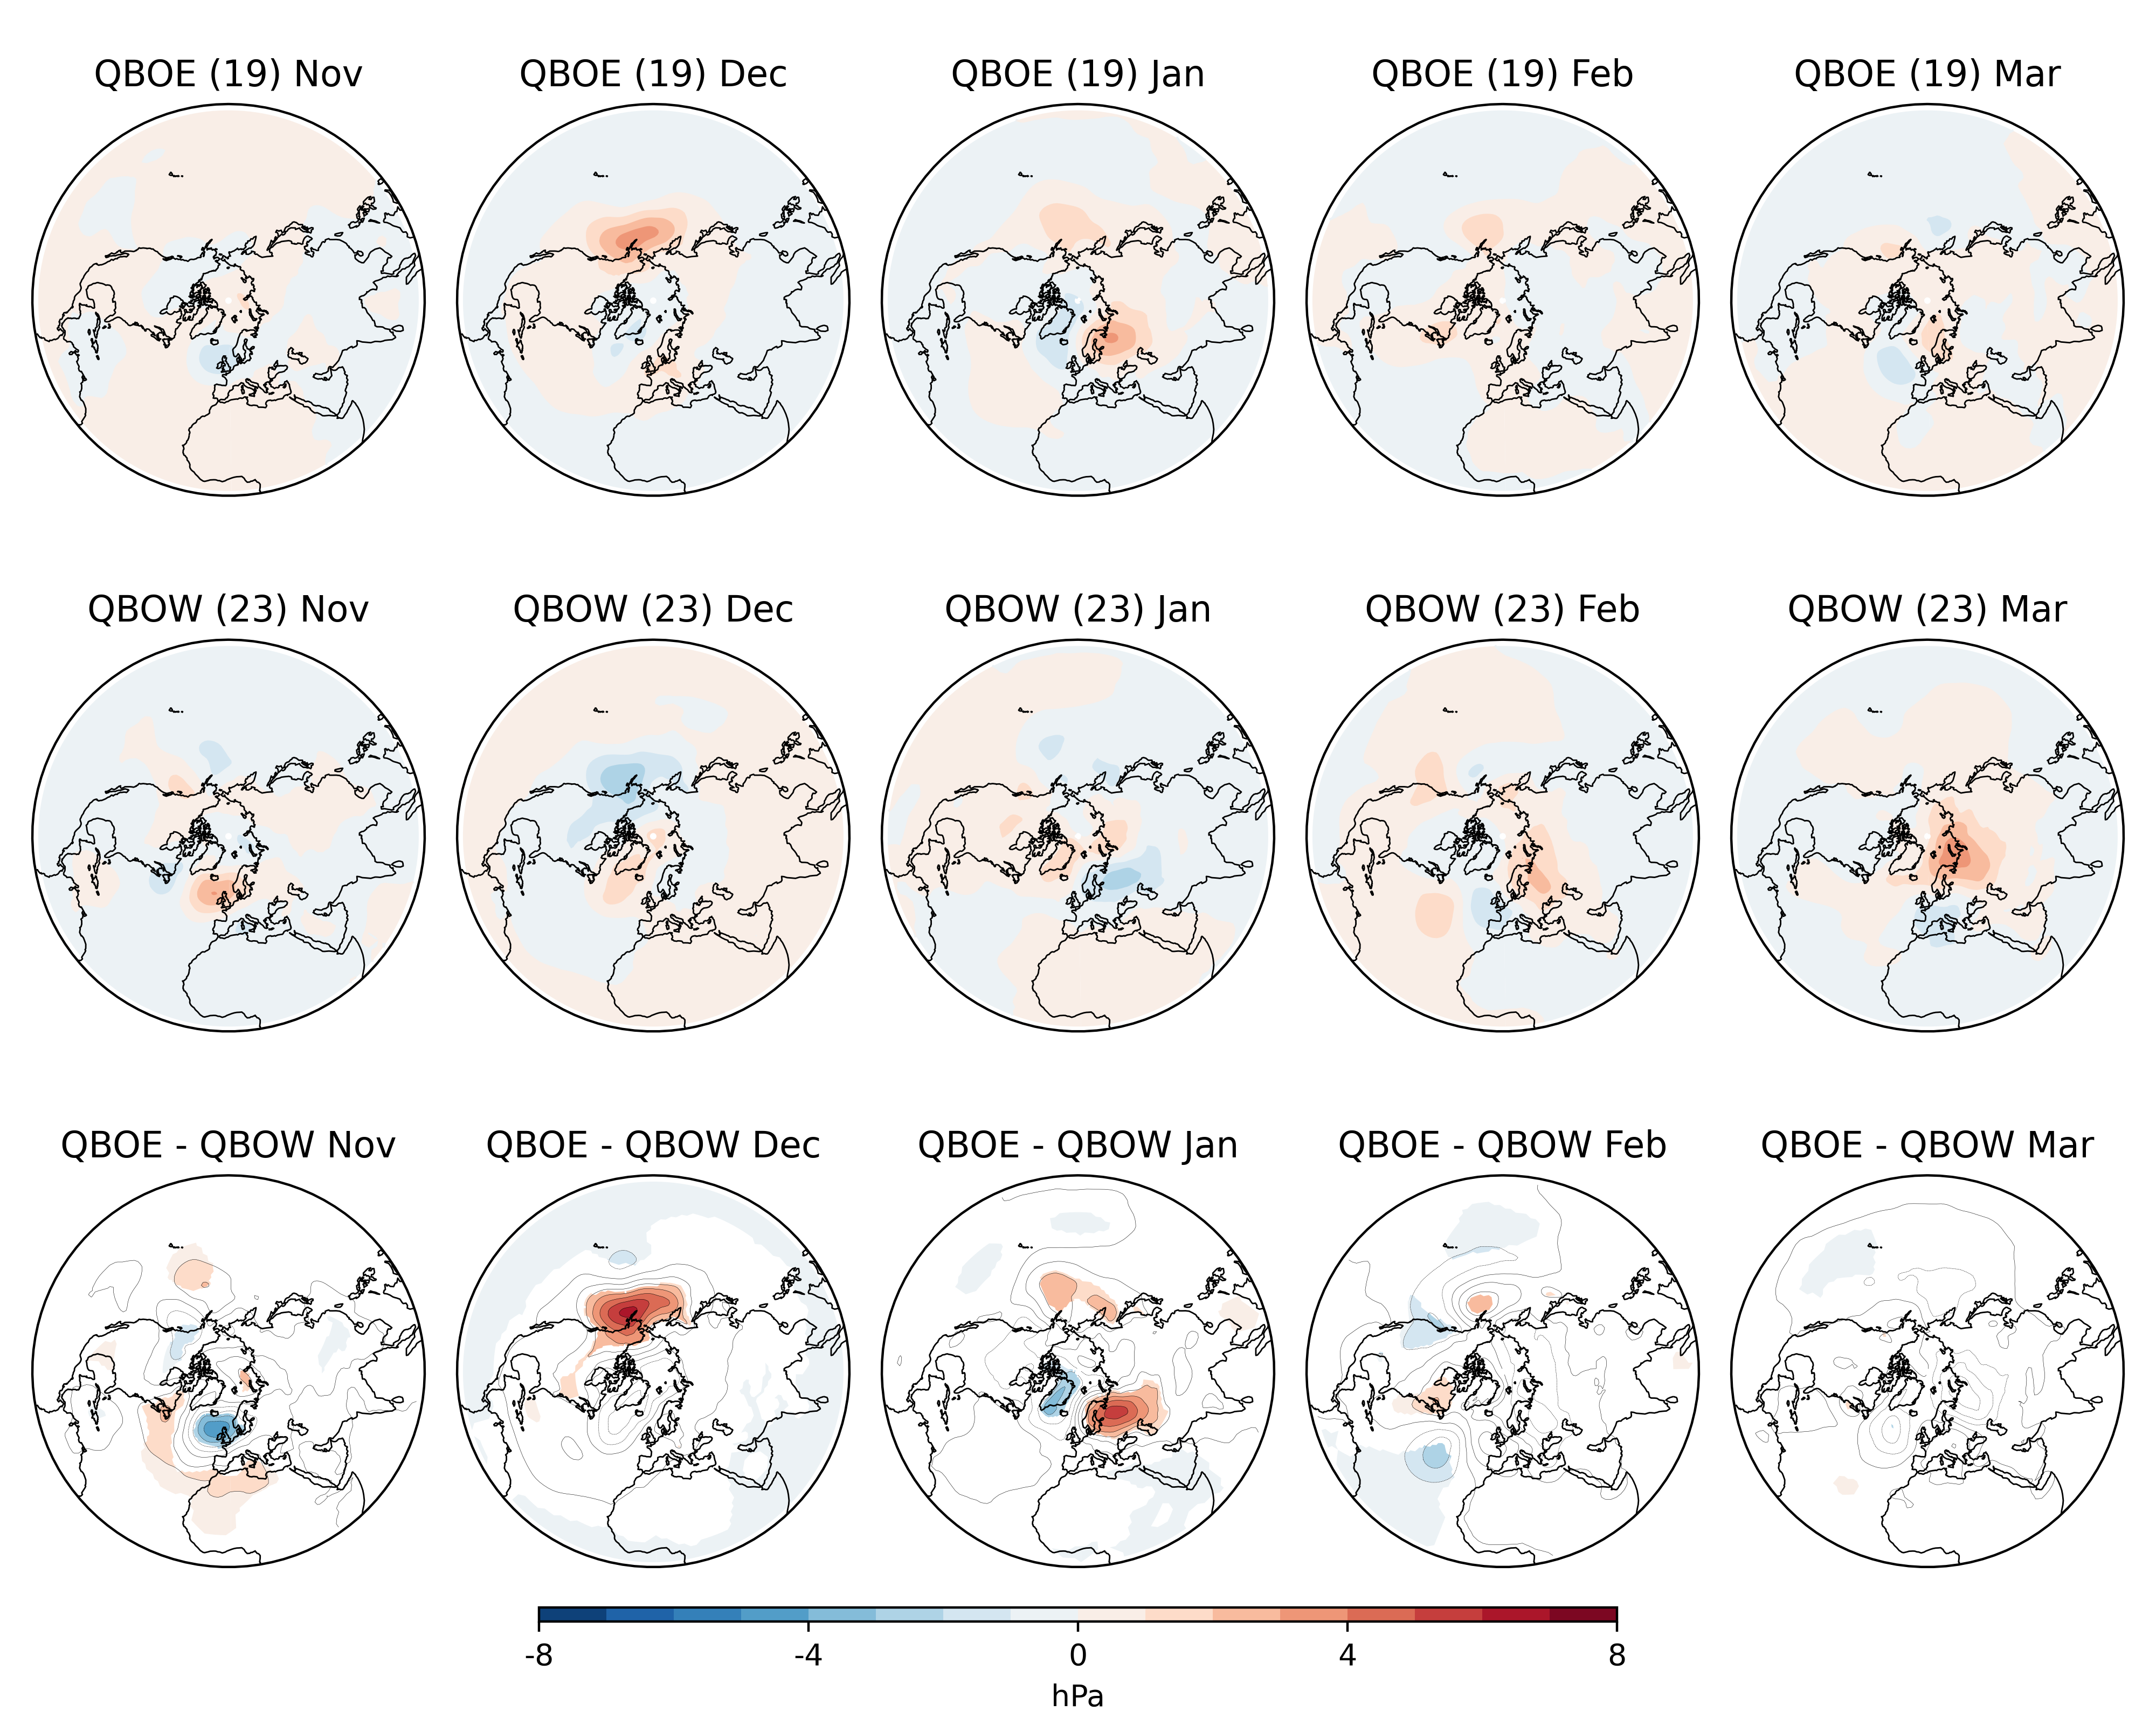
\includegraphics[width =0.8\linewidth]{Figures/Figures-deepQBO/LAGGED_SLP_composites_individual_months_QBO_phases_U_piclim_50hPa_5thresh.png}
\caption[MSLP composites under different QBO phases in the pi-clim cntrl simulation]{NH deseasonalised MSLP anomaly composites for the QBO East (top row), QBO West (middle row) phases and composite differences (QBOE - QBOW, bottom row) for the pi-clim cntrl simulation. The QBO phase is defined as any Nov-Dec mean equatorial ($5^{\circ}$\ S--$5^{\circ}\ $N average) ZMZW on the 50 hPa that exceeds a magnitude of $5 ms^{-1}$, i.e. $+5 ms^{-1}$ threshold for QBOW and $-5 ms^{-1}$ threshold for QBOE. Anomalies associated with each QBO phase are presented in various months which are indicated in sub-figure titles. Numbers in parentheses indicate the number of NH winters that occur under each phase which make up the composite. Coloured shading in the bottom row indicates MSLP differences significant above the 95\% confidence level under a 2 tail student’s t-test.}
\label{fig:SLP_piclim}
\end{center}
\end{figure}

In early winter (Nov), the response to the QBO is marginal; there is a significant positive differences in MSLP for QBOE-QBOW over the Icelandic region which corresponds to a negative NAO however this covers a relatively small region compared to some of the same composites presented in \cite{andrewsObserved2019d} and \cite{graySurface2018b} that show a coherent NAO response to the 50 hPa QBO in ERA-Interim that peaks in January. In mid-winter (Dec-Feb), the composite differences do not resemble a coherent NAO/AO pattern with the exception of responses in December which exhibit positive differences over the AL region. A QBO signal is also absent in later winter (Mar), a month in which \cite{graySurface2018b} highlight a coherent Pacific MSLP response in ERA-Interim. These disparate patterns are not significantly altered by the exclusion of NH winters which exhibit November SSWs (not shown) suggesting the lack of signal is likely not linked to the model SSW bias seen in figure \ref{fig:SSW_histogram_experiments}. 

In contrast, the corresponding MSLP composites from the deep experiment (figure \ref{fig:SLP_deep}) exhibit a prominent signal in the NAO region indicated by a significant composite difference of up to 8 hPa over the North Atlantic region. This signal is most apparent in mid-late winter (Jan-Mar), although a similar anomaly is visible in November. This feature corresponds to positive (negative) MSLP anomalies under QBOE (QBOW) conditions centred over the southern node of the NAO (a region encompassing the Azores). As with the pi-clim cntrl, there is a small discrepancy in the abundance of winters exhibiting different QBO phases with the QBOW phase marginally more prominent. However, this difference is small and indicates that the asymmetry in phase amplitudes demonstrated in figure \ref{fig:experiment_QBOs} has not had a significant impact on the preferential occurrence of NH winters under each phase.

These patterns indicate a shift towards a positive NAO pattern under QBOE conditions and negative NAO under QBOW - the opposite sign to a response expected via a Holton-Tan mechanism which predicts a weakened (strengthened) vortex and subsequent negative (positive) NAO under QBOE (QBOW) phases. Furthermore, \cite{andrewsObserved2019d} show a response consistent with a Holton-Tan link and of the opposite sign to those shown here (positive NAO phase under QBOW conditions) using a deep QBO metric in observations and a free-running model. As a result, our results are somewhat surprising and warrant further study into their origins which is presented in the following sections.
\begin{figure}[h!]
\begin{center}
\noindent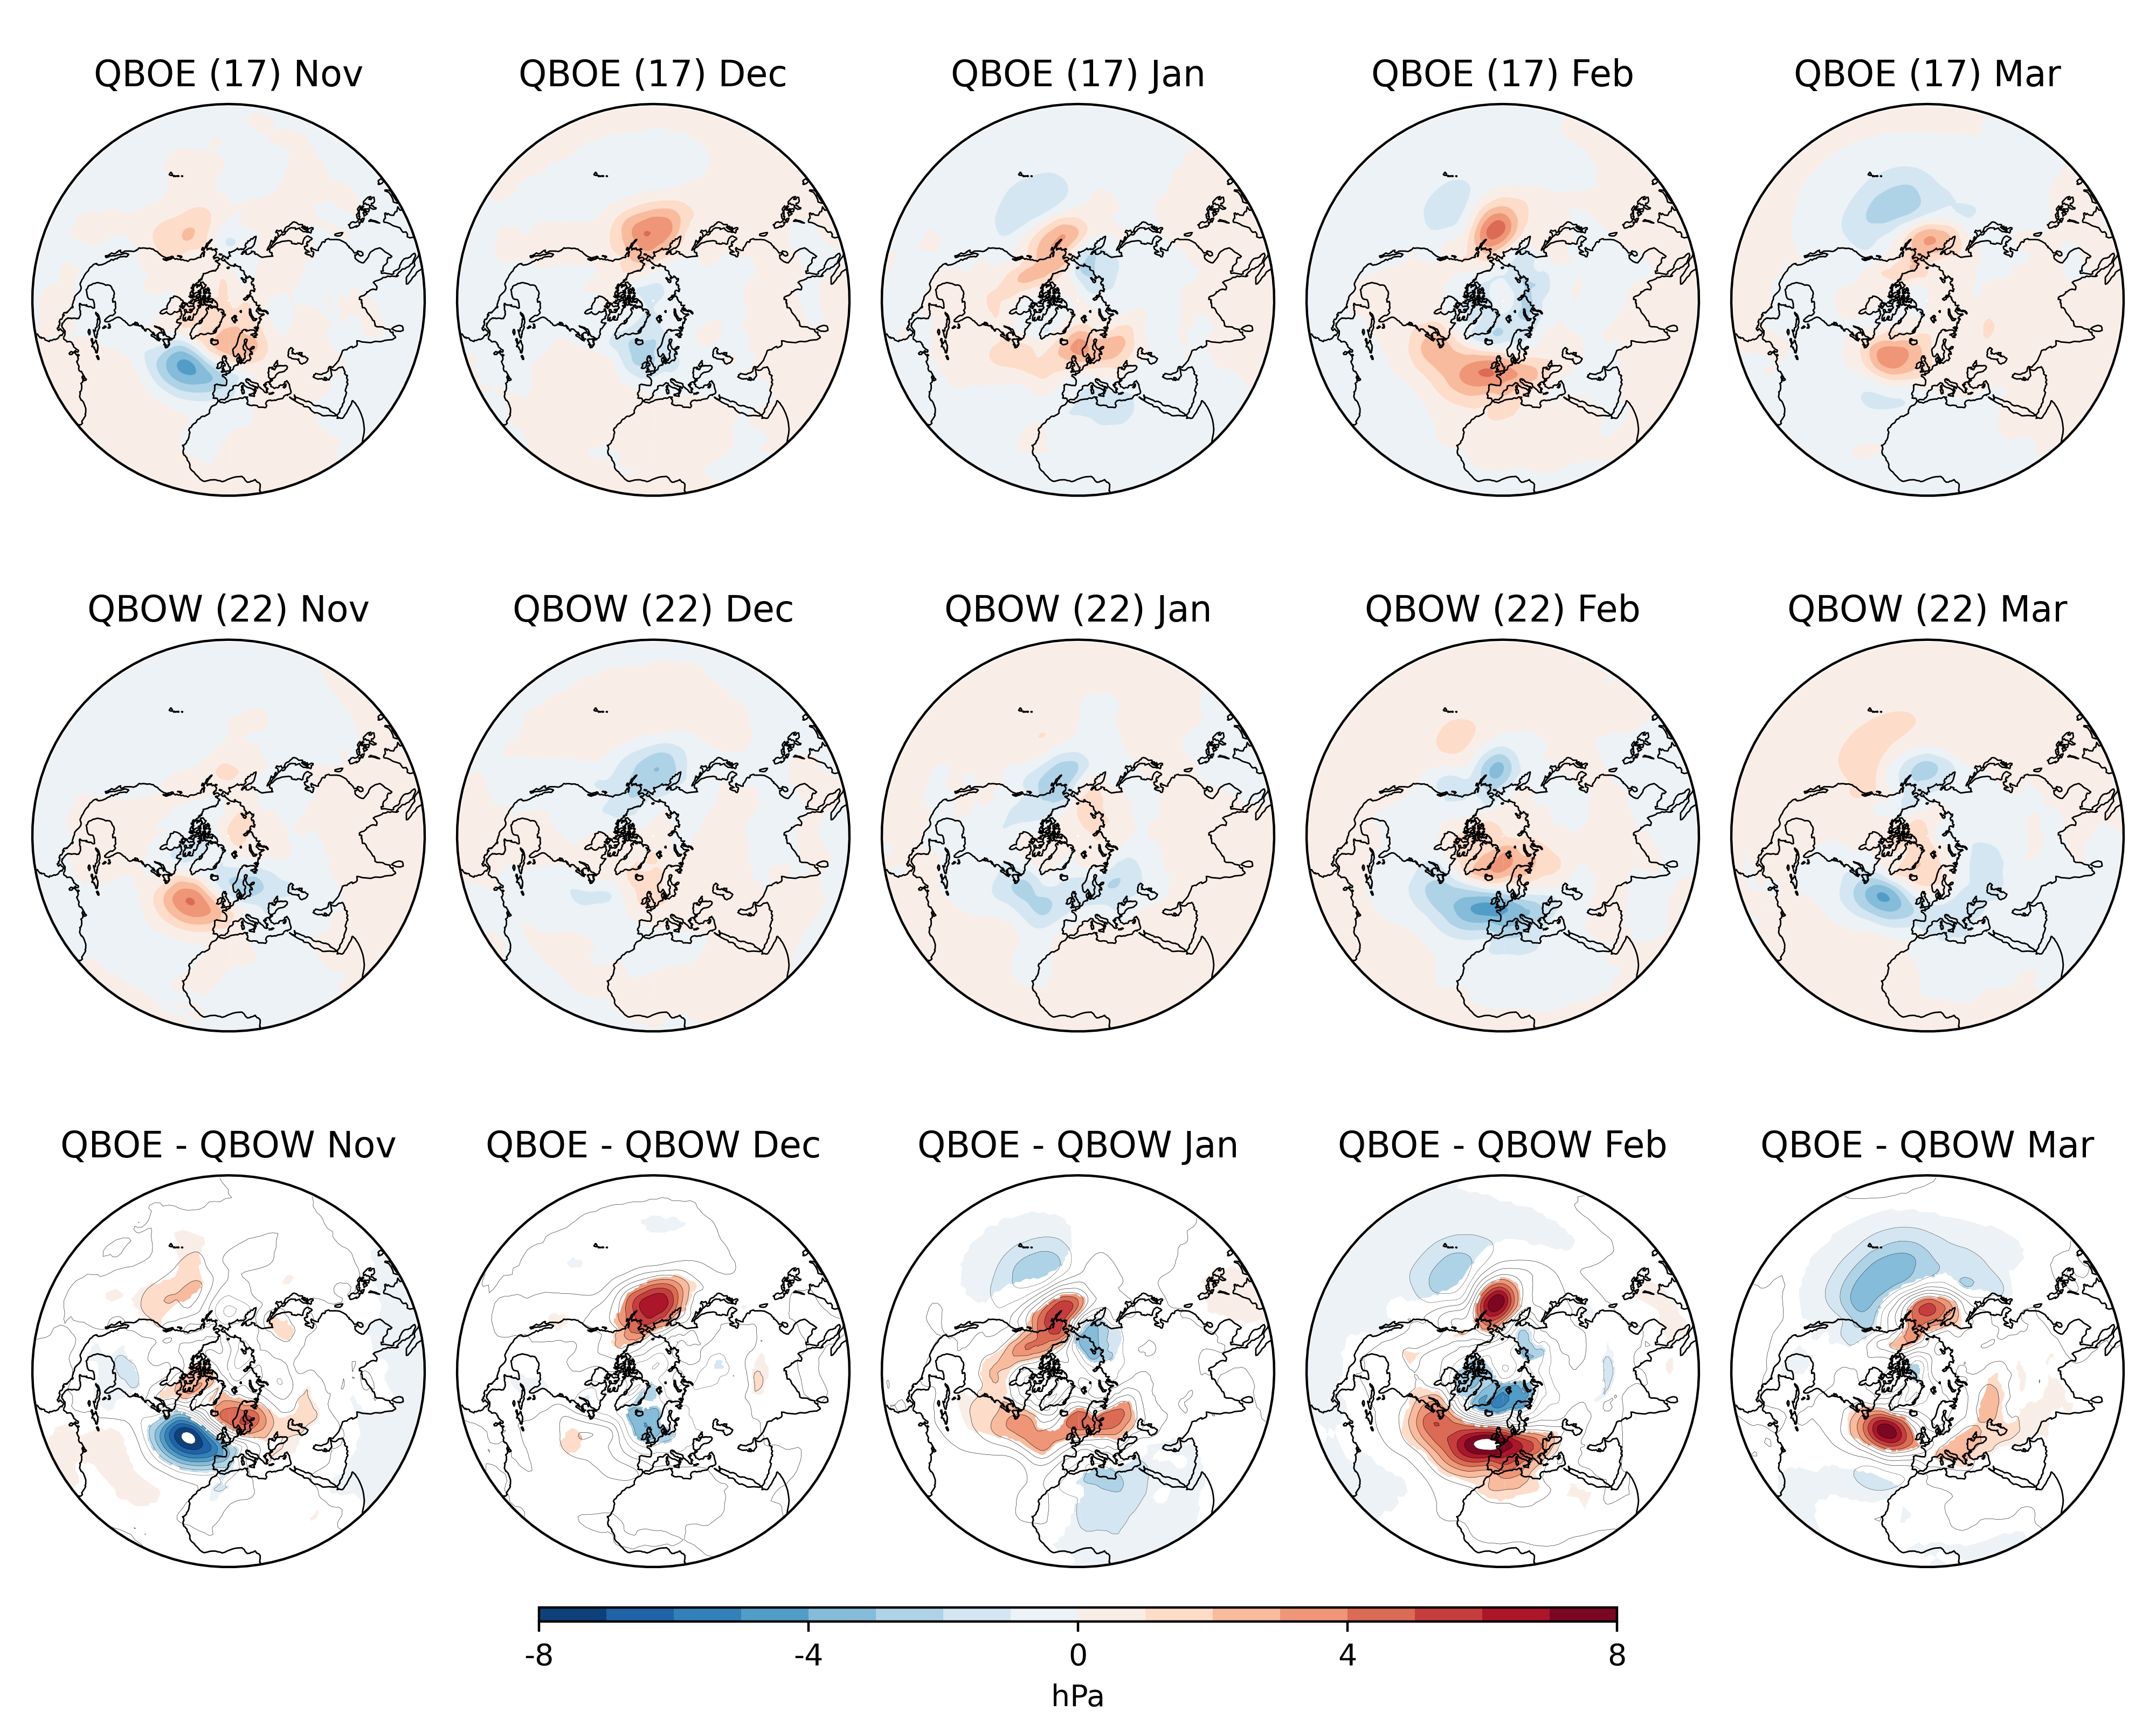
\includegraphics[width =0.8\linewidth]{Figures/Figures-deepQBO/LAGGED_SLP_composites_individual_months_QBO_phases_U_d_higher_50hPa_5thresh.png}
\caption[MSLP composites under different QBO phases in the deep QBO simulation]{Like figure \ref{fig:SLP_piclim} for the deep QBO experiment.}
\label{fig:SLP_deep}
\end{center}
\end{figure}

The corresponding Atlantic responses from the shallow QBO experiment (figure \ref{fig:SLP_shallow}) are markedly different to its deep counterpart: The magnitude of responses to individual QBO phases (top two rows) as well as differences (bottom row) are smaller than in the deep experiment (up to $\sim$4 hPa) and a smaller region of composite differences are deemed significant under a 2 tailed t-test (also bottom row). There is also a MSLP response in the North Pacific in both nudged experiments concentrated over the AL region which corresponds to the Pacific node of the AO (see figure \ref{fig:AO}). As with the Atlantic response, the deep experiment exhibits anomalies with larger amplitude than the those in the shallow. Both experiments' Pacific responses are most prominent in mid NH winter (Dec-Feb) consistent with similar findings in \cite{graySurface2018b} that show significant anomalies over this region peak in February. The sign of the anomalies in this region for both experiments indicate that a positive (negative) Pacific pattern corresponds to QBOE (QBOW) conditions; again, an opposite response to that seen in \cite{andrewsObserved2019d} and \cite{graySurface2018b}. As with the pi-clim cntrl, both experiment's MSLP responses are not significantly affected by the removal of November SSWs. Overall, results comparing MSLP composites in our two nudged experiments indicate enhanced amplitudes of response patterns to a perpetually deep QBO. However, the Atlantic and Pacific responses in the deep experiment is of the opposite sign to the expected HT mechanism as well as that in \citep{andrewsObserved2019d} and therefore a closer examination of possible pathways involved in this response is required to understand the role of vertical coherence in the QBO in our simulations.

\begin{figure}[h!]
\begin{center}
\noindent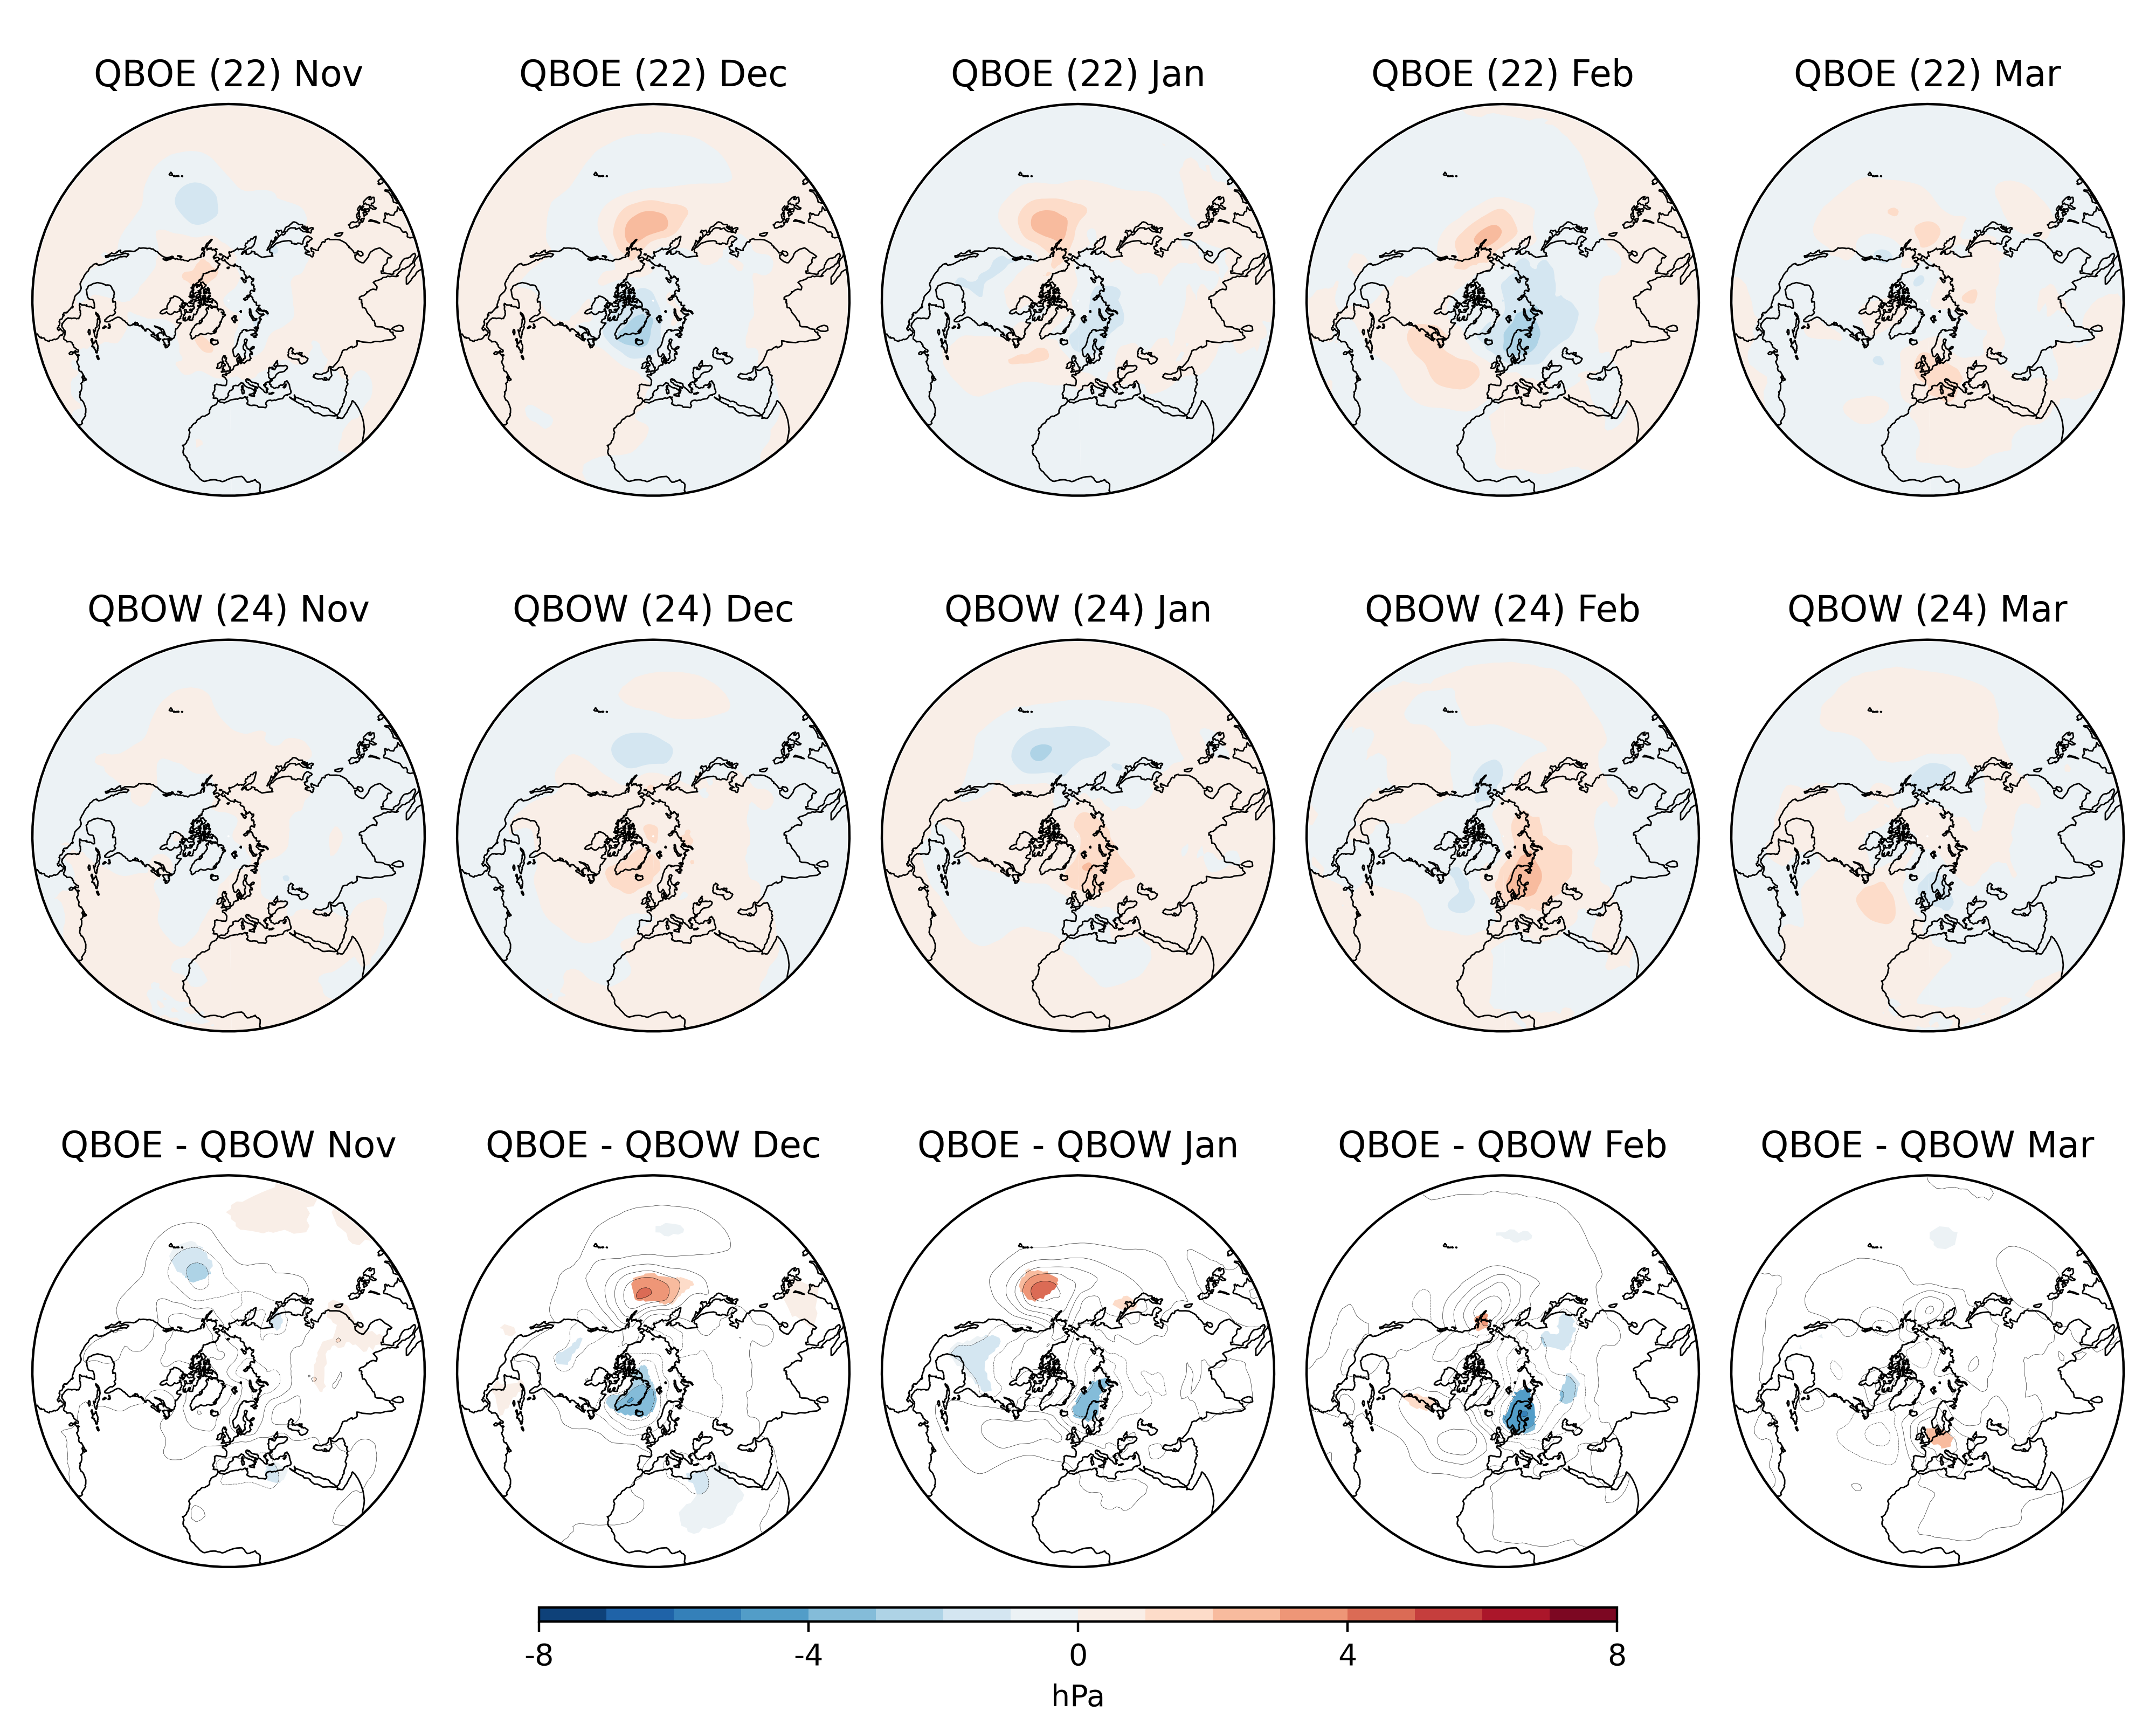
\includegraphics[width =0.8\linewidth]{Figures/Figures-deepQBO/LAGGED_SLP_composites_individual_months_QBO_phases_U_s_50hPa_5thresh.png}
\caption[MSLP composites under different QBO phases in the shallow QBO simulation]{Like figure \ref{fig:SLP_piclim} for the shallow QBO experiment.}
\label{fig:SLP_shallow}
\end{center}
\end{figure}
\newpage

\section{Vortex responses to the QBO}
\label{sec:vortex_responses_QBO}
We next analyse the interaction between the QBO and the vortex in each experiment to further understand the possible mechanisms involved in the surface responses seen in the previous section. Figure \ref{fig:HT_piclim} shows a measure of the strength of the Holton-Tan effect in the pi-clim cntrl simulation - composite differences between NH winter ZMZW under QBOE and QBOW conditions. The phase of the QBO is defined in early winter (Nov-Dec) on various pressure levels (rows in figure \ref{fig:HT_piclim}) and ZMZW differences are evaluated for a range of NH winter months (columns). The response from the vortex in this un-nudged simulation broadly reflects the composites from the fully coupled pi-control simulation of UKESM (figure \ref{fig:holton_tan_comp}) with negative composite differences in the vortex when the QBO is defined on the 20 hPa and 30 hPa levels. This is consistent with the HT effect discussed in section \ref{sec:external_influence_HT} in which the easterly QBO phase is associated with a weakened vortex (see figure \ref{fig:HT_piclim}, left column). The majority of these negative differences are concentrated in early-mid winter months (Nov-Jan), a finding also reported in \cite{graySurface2018b}. There are negative composite differences to the QBO at 70 hPa and 50 hPa also in early winter which extend from the subtropics to as far north as 50$\degree$N. In late winter (Feb-Mar), the response of the vortex reduces and even reverse to positive on the 70 hPa level (again, an effect reported in \cite{graySurface2018b}). The equatorial anomalies associated with QBO phases in this simulation are characterised by a four-fold structure in height with alternating QBOE/W phases evident throughout the mid-stratosphere and extending into the lower-mesosphere.

\newpage
\begin{figure}[h!]
\begin{center}
\noindent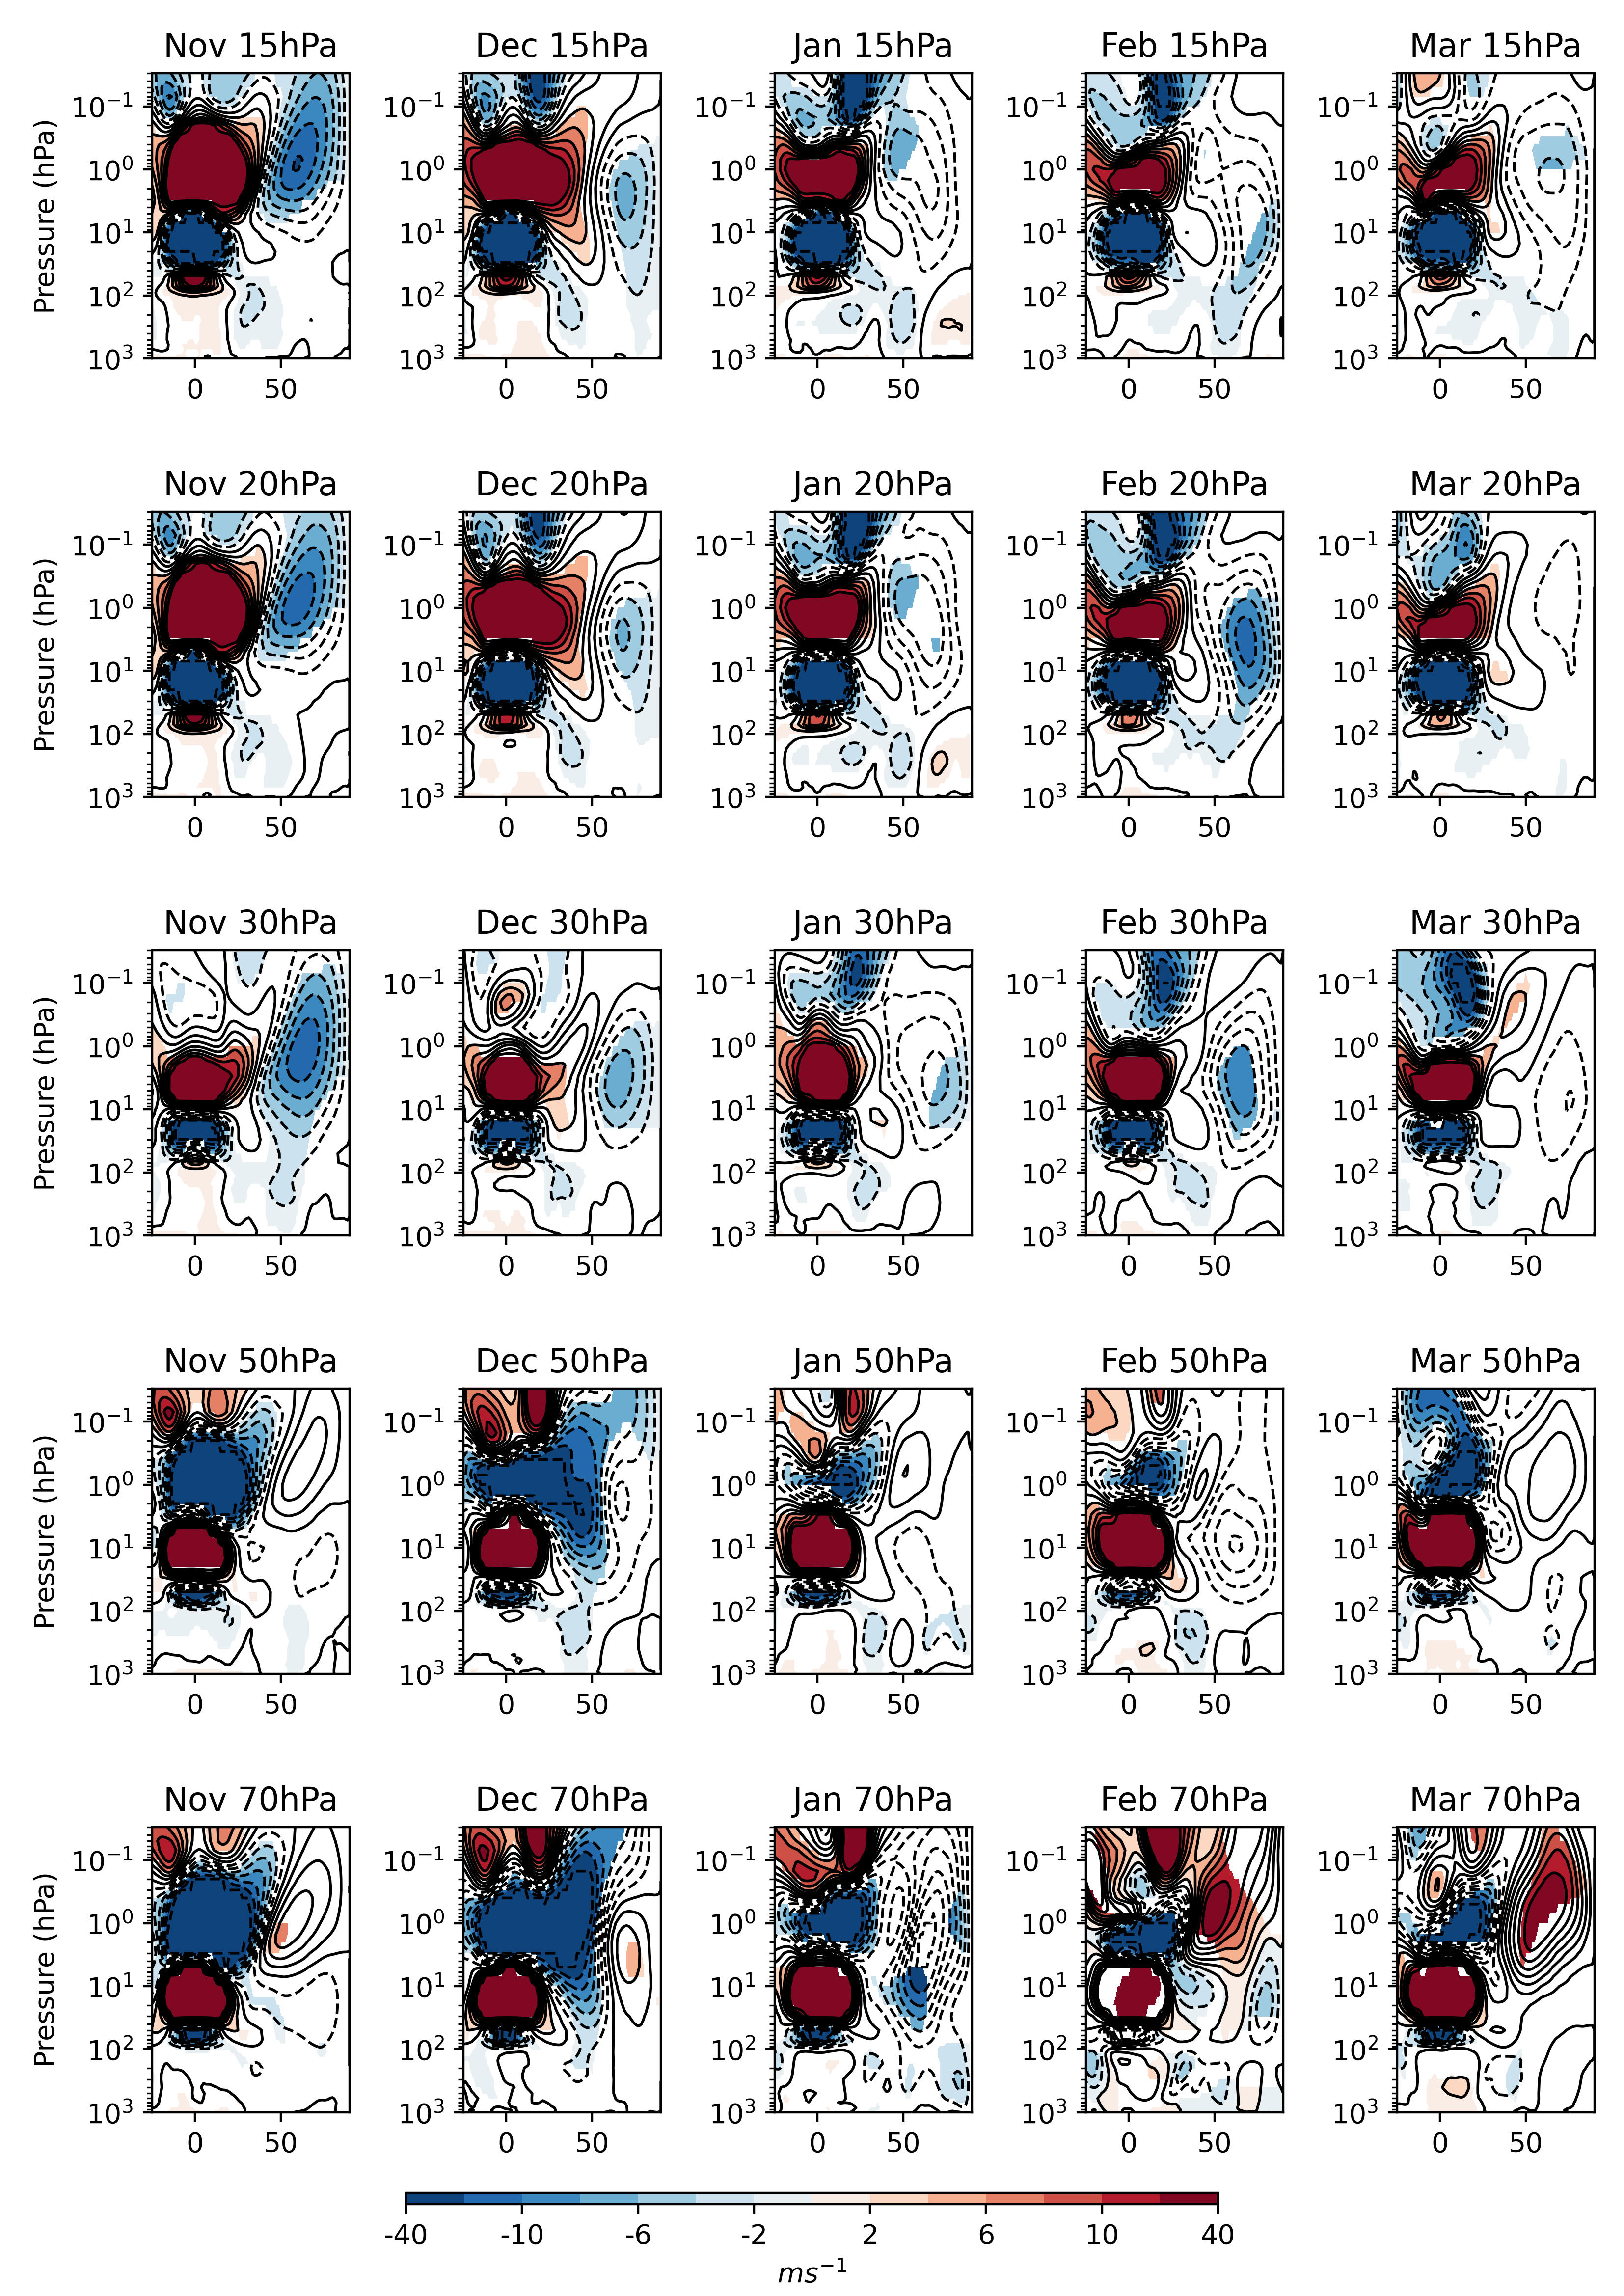
\includegraphics[width = 0.82\linewidth]{Figures/Figures-deepQBO/ZMZW_composites_by_month_QBO_phases_U_piclim_MarQBO_vs_Mar_70hPa_5thresh.png}
\caption[ZMZW composites under different QBO phases in the pi-clim cntrl simulation]{ZMZW composite differences for QBOE - QBOW conditions from the pi-clim cntrl simulation. The QBO phase is defined as any Nov-Dec mean equatorial ($5^{\circ}$\ S--$5^{\circ}\ $N average) ZMZW on the 50 hPa that exceeds a magnitude of $5 ms^{-1}$, i.e. $+5 ms^{-1}$ threshold for QBOW and $-5 ms^{-1}$ threshold for QBOE on various pressure levels which are indicated by sub-figure titles. Differences are evaluated in a range of NH winter months (also indicated in sub-figure titles). Coloured shading indicates ZMZW differences significant above the 95\% confidence level under a 2 tail student’s t-test.}
\label{fig:HT_piclim}
\end{center}
\end{figure}
\newpage
The pi-clim cntrl composites also reflect some of the key features of corresponding ZMZW responses from ERA-Interim (figure \ref{fig:HT_ERA}). Namely, the ERA-Interim composites also exhibit a seasonal progression with negative composite differences for QBOE-QBOW which increase from November and peak in January before reversing in March. However, the amplitude of vortex responses in the model is weaker than in ERA-Interim, which is in common with other models \citep{ansteyTeleconnections2021}, although it's not clear whether this is due to a true underestimation of the response by the models or whether it is due to to internal variability since the strength of the observed HT effect has been shown to vary over time (e.g. \cite{luDecadalscale2008c} and \cite{luMechanisms2014c}. ERA-Interim responses are also most prominent using a QBO metric defined on the 50 hPa level in contrast to the model which exhibits largest responses to the QBO defined at a higher level (20 hPa and 30 hPa). This discrepancy is seen in many models studied under QBOI (see section \ref{sec:equatorial_strat}) and attributed to QBO phases in GCMs that fail to penetrate down with a large enough amplitude to the 50 hPa level \citep{ansteyTeleconnections2021}. Nevertheless, the pi-clim cntrl composites indicate that the un-nudged configuration of the model is able to reproduce a clear coupling between the QBO and the vortex suggesting the suitability of this model configuration for QBO-vortex analysis with nudged QBO simulations.

\newpage 
\begin{figure}[h!]
\begin{center}
\noindent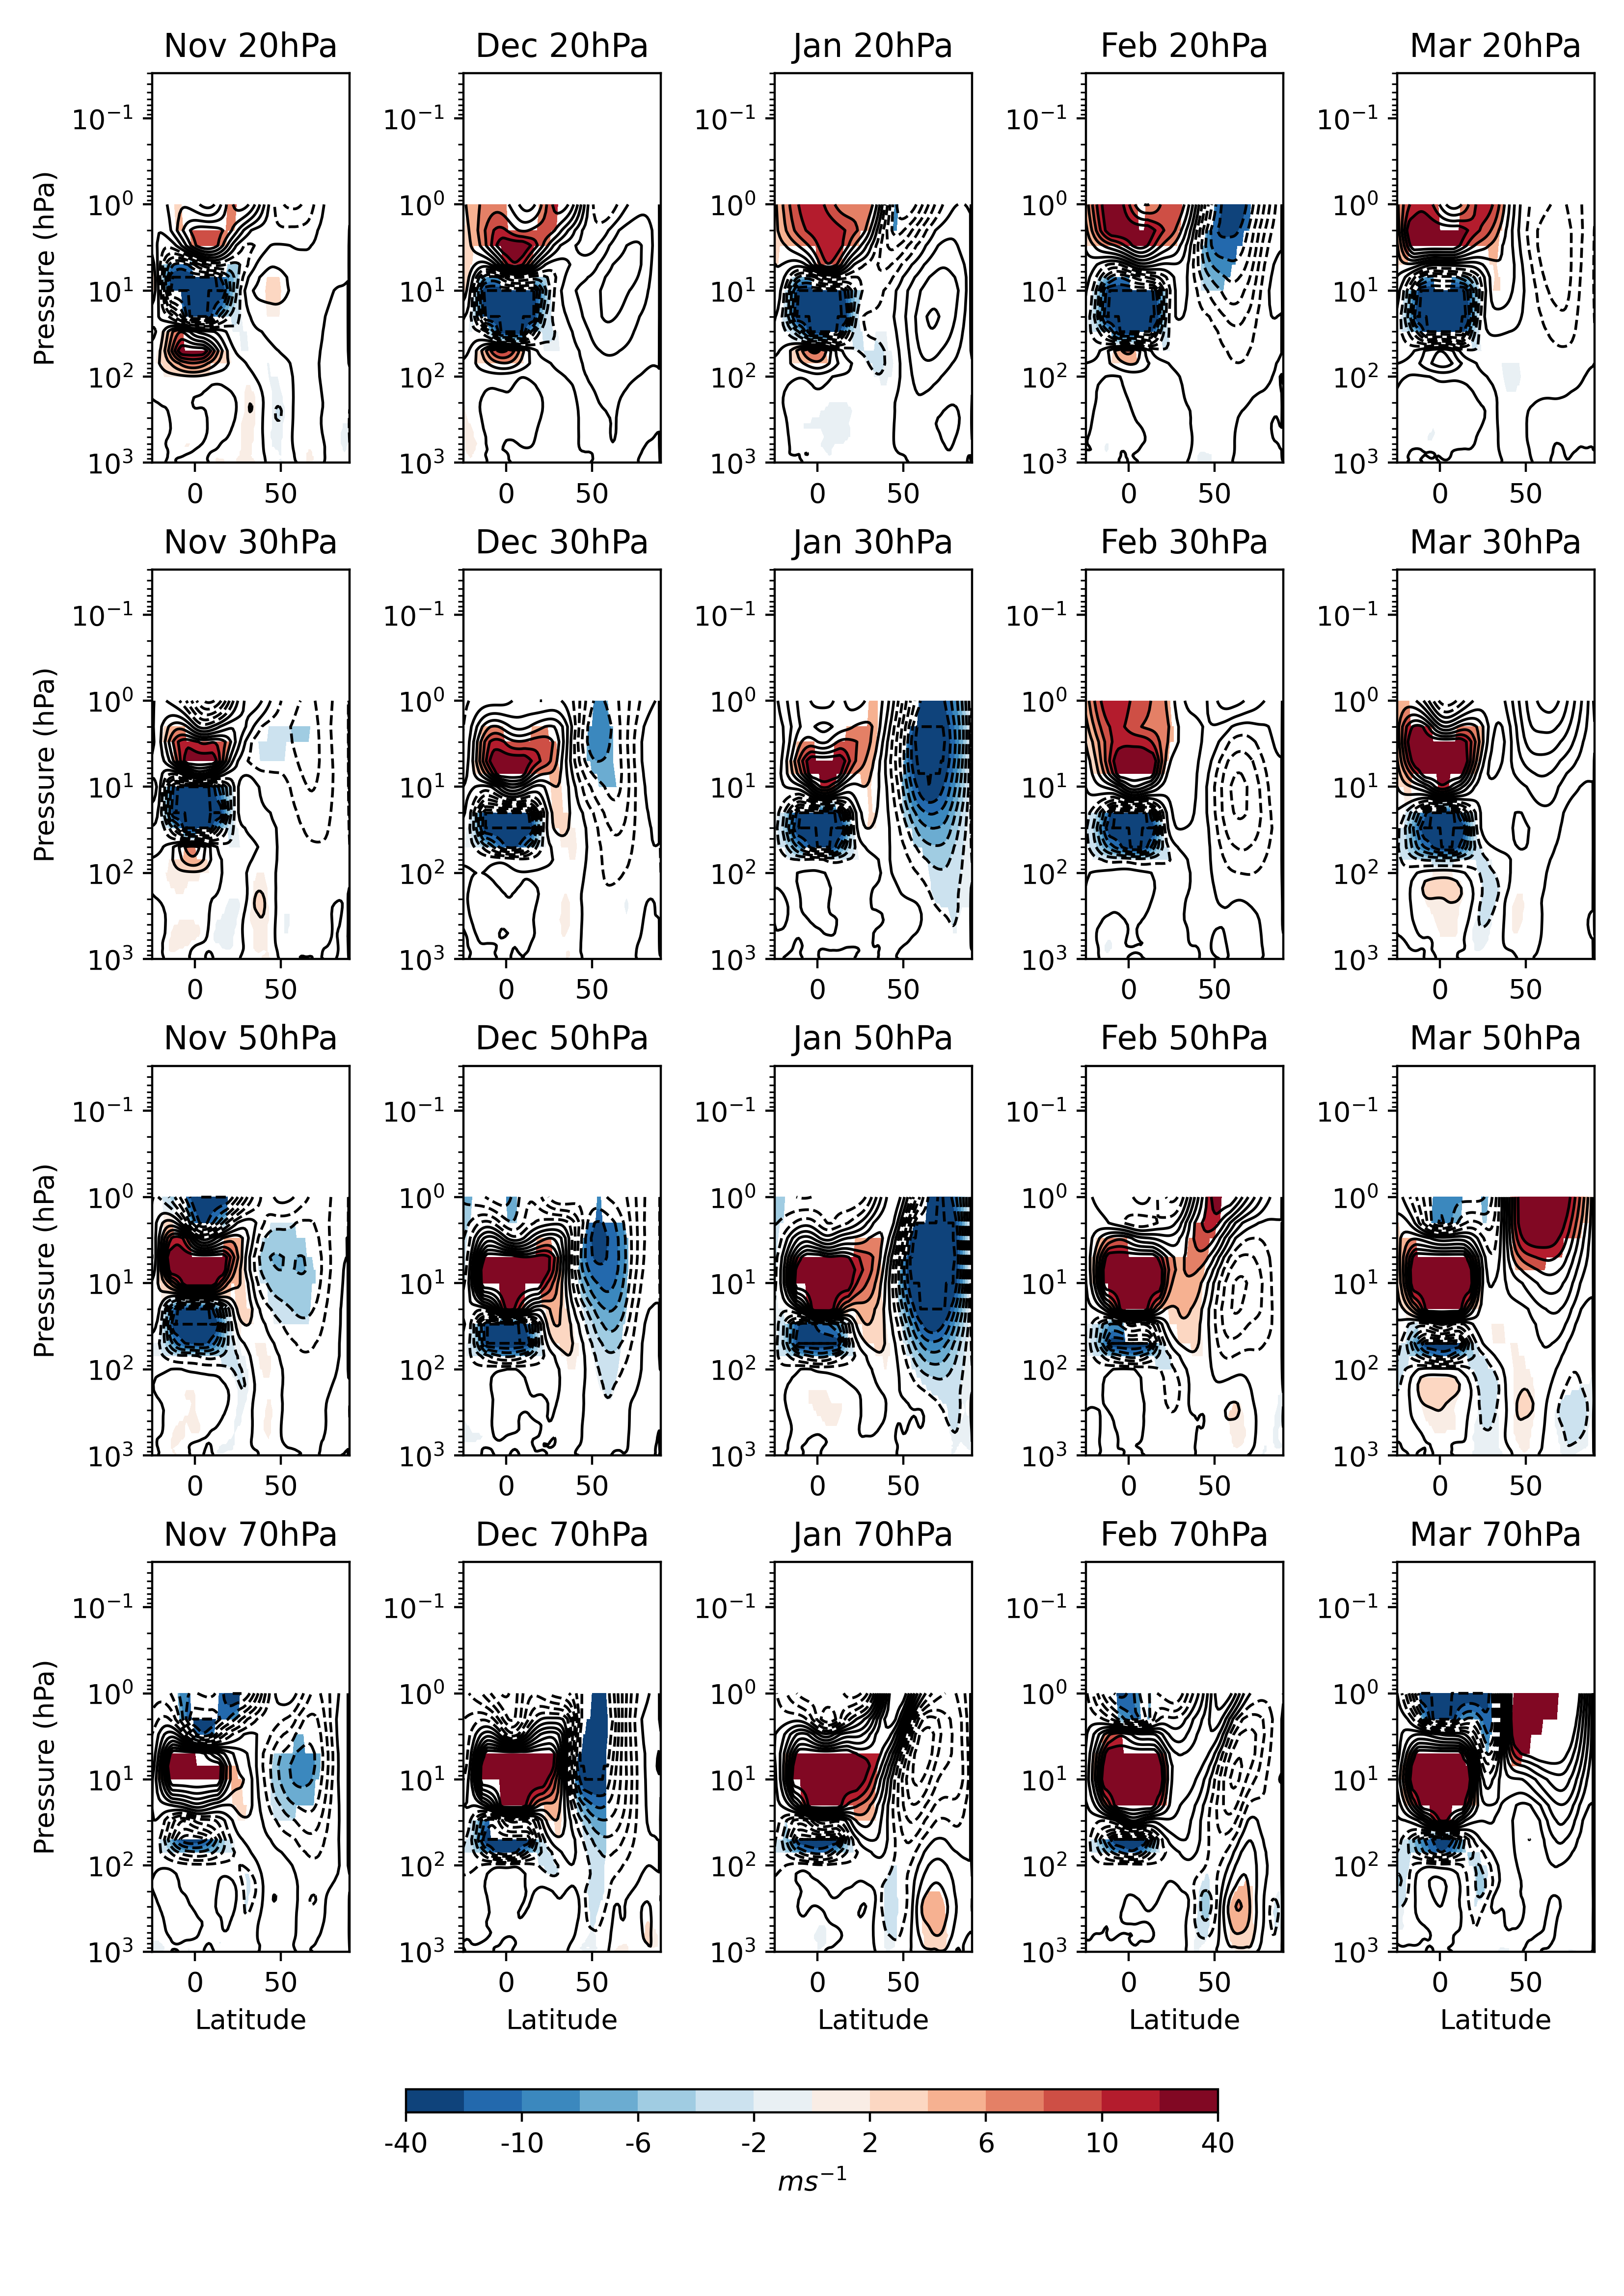
\includegraphics[width = 0.85\linewidth]{Figures/Figures-deepQBO/LAGGED_ZMZW_composites_by_month_QBO_phases_U_ERA_MarQBO_vs_Mar_70hPa_5thresh.png}
\caption[ZMZW composites under different QBO phases in ERA-Interim]{Like figure \ref{fig:HT_piclim} for ERA-Interim. Composites for the QBO defined on the 15 hPa level are not included as this is not a standard level output for ERA-Interim. }
\label{fig:HT_ERA}
\end{center}
\end{figure}

The corresponding ZMZW composite differences between QBO phases in the deep and shallow QBO experiments (figure \ref{fig:HT_deep} and \ref{fig:HT_shallow} respectively) show distinct response patterns. In early winter (November), both simulations exhibit negative composite differences in the vortex for QBOE - QBOW, in good agreement with a HT mechanism \citep{HoltonJamesRTan1980} as well as the pi-clim cntrl (figure \ref{fig:HT_piclim}). The magnitude of vortex responses in November is marginally larger in the deep experiment compared to that of the shallow and pi-clim cntrl. The equatorial response patterns in the deep experiment predominantly exhibit a two-fold structure in early winter (Nov-Dec) with anomalies in the lower-mid stratosphere and opposite anomalies above in the upper stratosphere and lower mesosphere. In later winter (Jan-Mar), an additional phase above the 0.1 hPa level is evident forming a three-fold structure. The corresponding equatorial responses in the shallow experiment shows a combination of two, three and four-fold patterns of anomalies. 

In mid-late winter (Jan-Mar), the deep experiment exhibits remarkably large positive composite differences in the vortex region. This notable feature is largely absent in the pi-clim cntrl (figure \ref{fig:HT_piclim}) as well as the shallow experiment (figure \ref{fig:HT_shallow}). There is a response to the QBO at 30 hPa in the shallow experiment with positive differences evident for February and March but these are significantly smaller in magnitude than those in the deep QBO simulation. These positive differences in the deep experiment are of the opposite sign to the expected HT relation however they do reflect the seasonal progression between early and later NH winter in QBO-vortex interactions suggested in \cite{graySurface2018b}. This seasonal progression in both experiments is unaffected by the removal of November SSWs and may also account for the positive (negative) NAO pattern MSLP responses to QBOE (QBOW) in late NH winter in figure \ref{fig:SLP_deep}: In these months, the vortex appears strengthened (weakened) under QBOE (QBOW) conditions which may in turn induce a positive (negative) NAO through the vortex's in-season influence over the NAO \citep{baldwinStratospheric2001a, charlton-perezInfluence2018e}. 

\newpage
\begin{figure}[h!]
\begin{center}
\noindent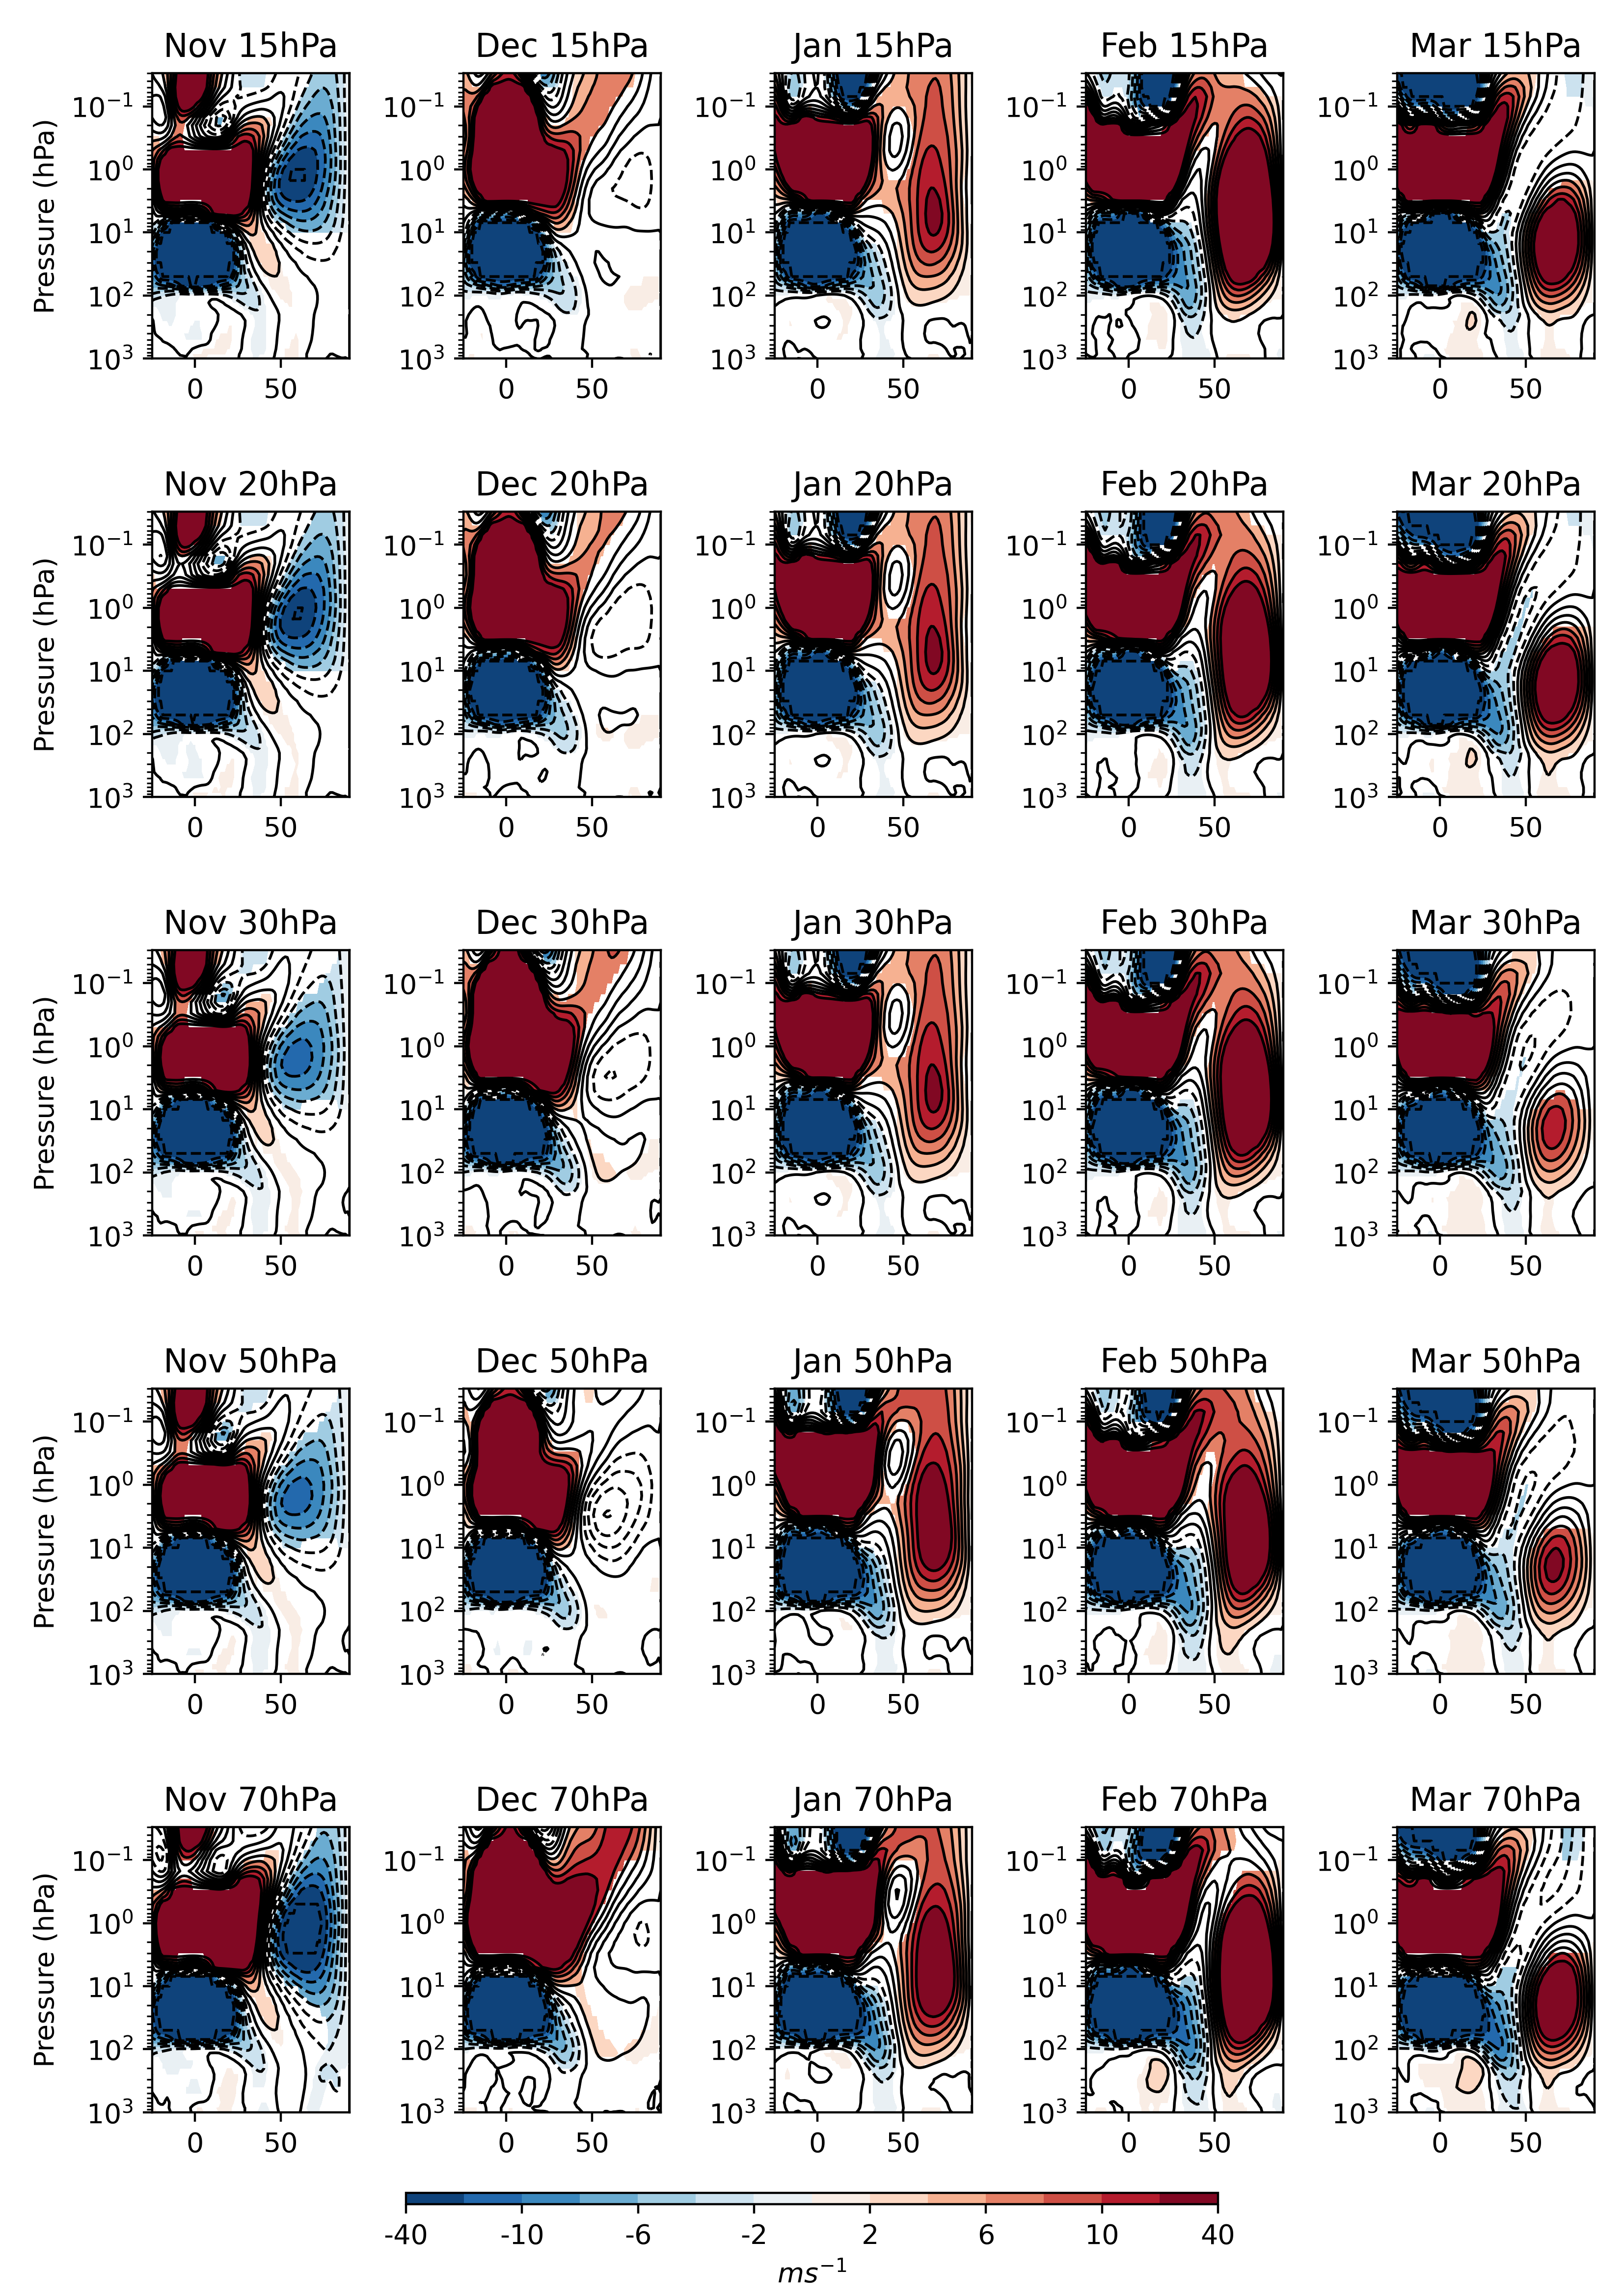
\includegraphics[width = 0.9\linewidth]{Figures/Figures-deepQBO/ZMZW_composites_by_month_QBO_phases_U_d_higher_MarQBO_vs_Mar_70hPa_5thresh.png}
\caption[ZMZW composites under different QBO phases in the deep QBO simulation]{Like figure \ref{fig:HT_piclim} for the deep experiment}
\label{fig:HT_deep}
\end{center}
\end{figure}
\newpage 

\begin{figure}[h!]
\begin{center}
\noindent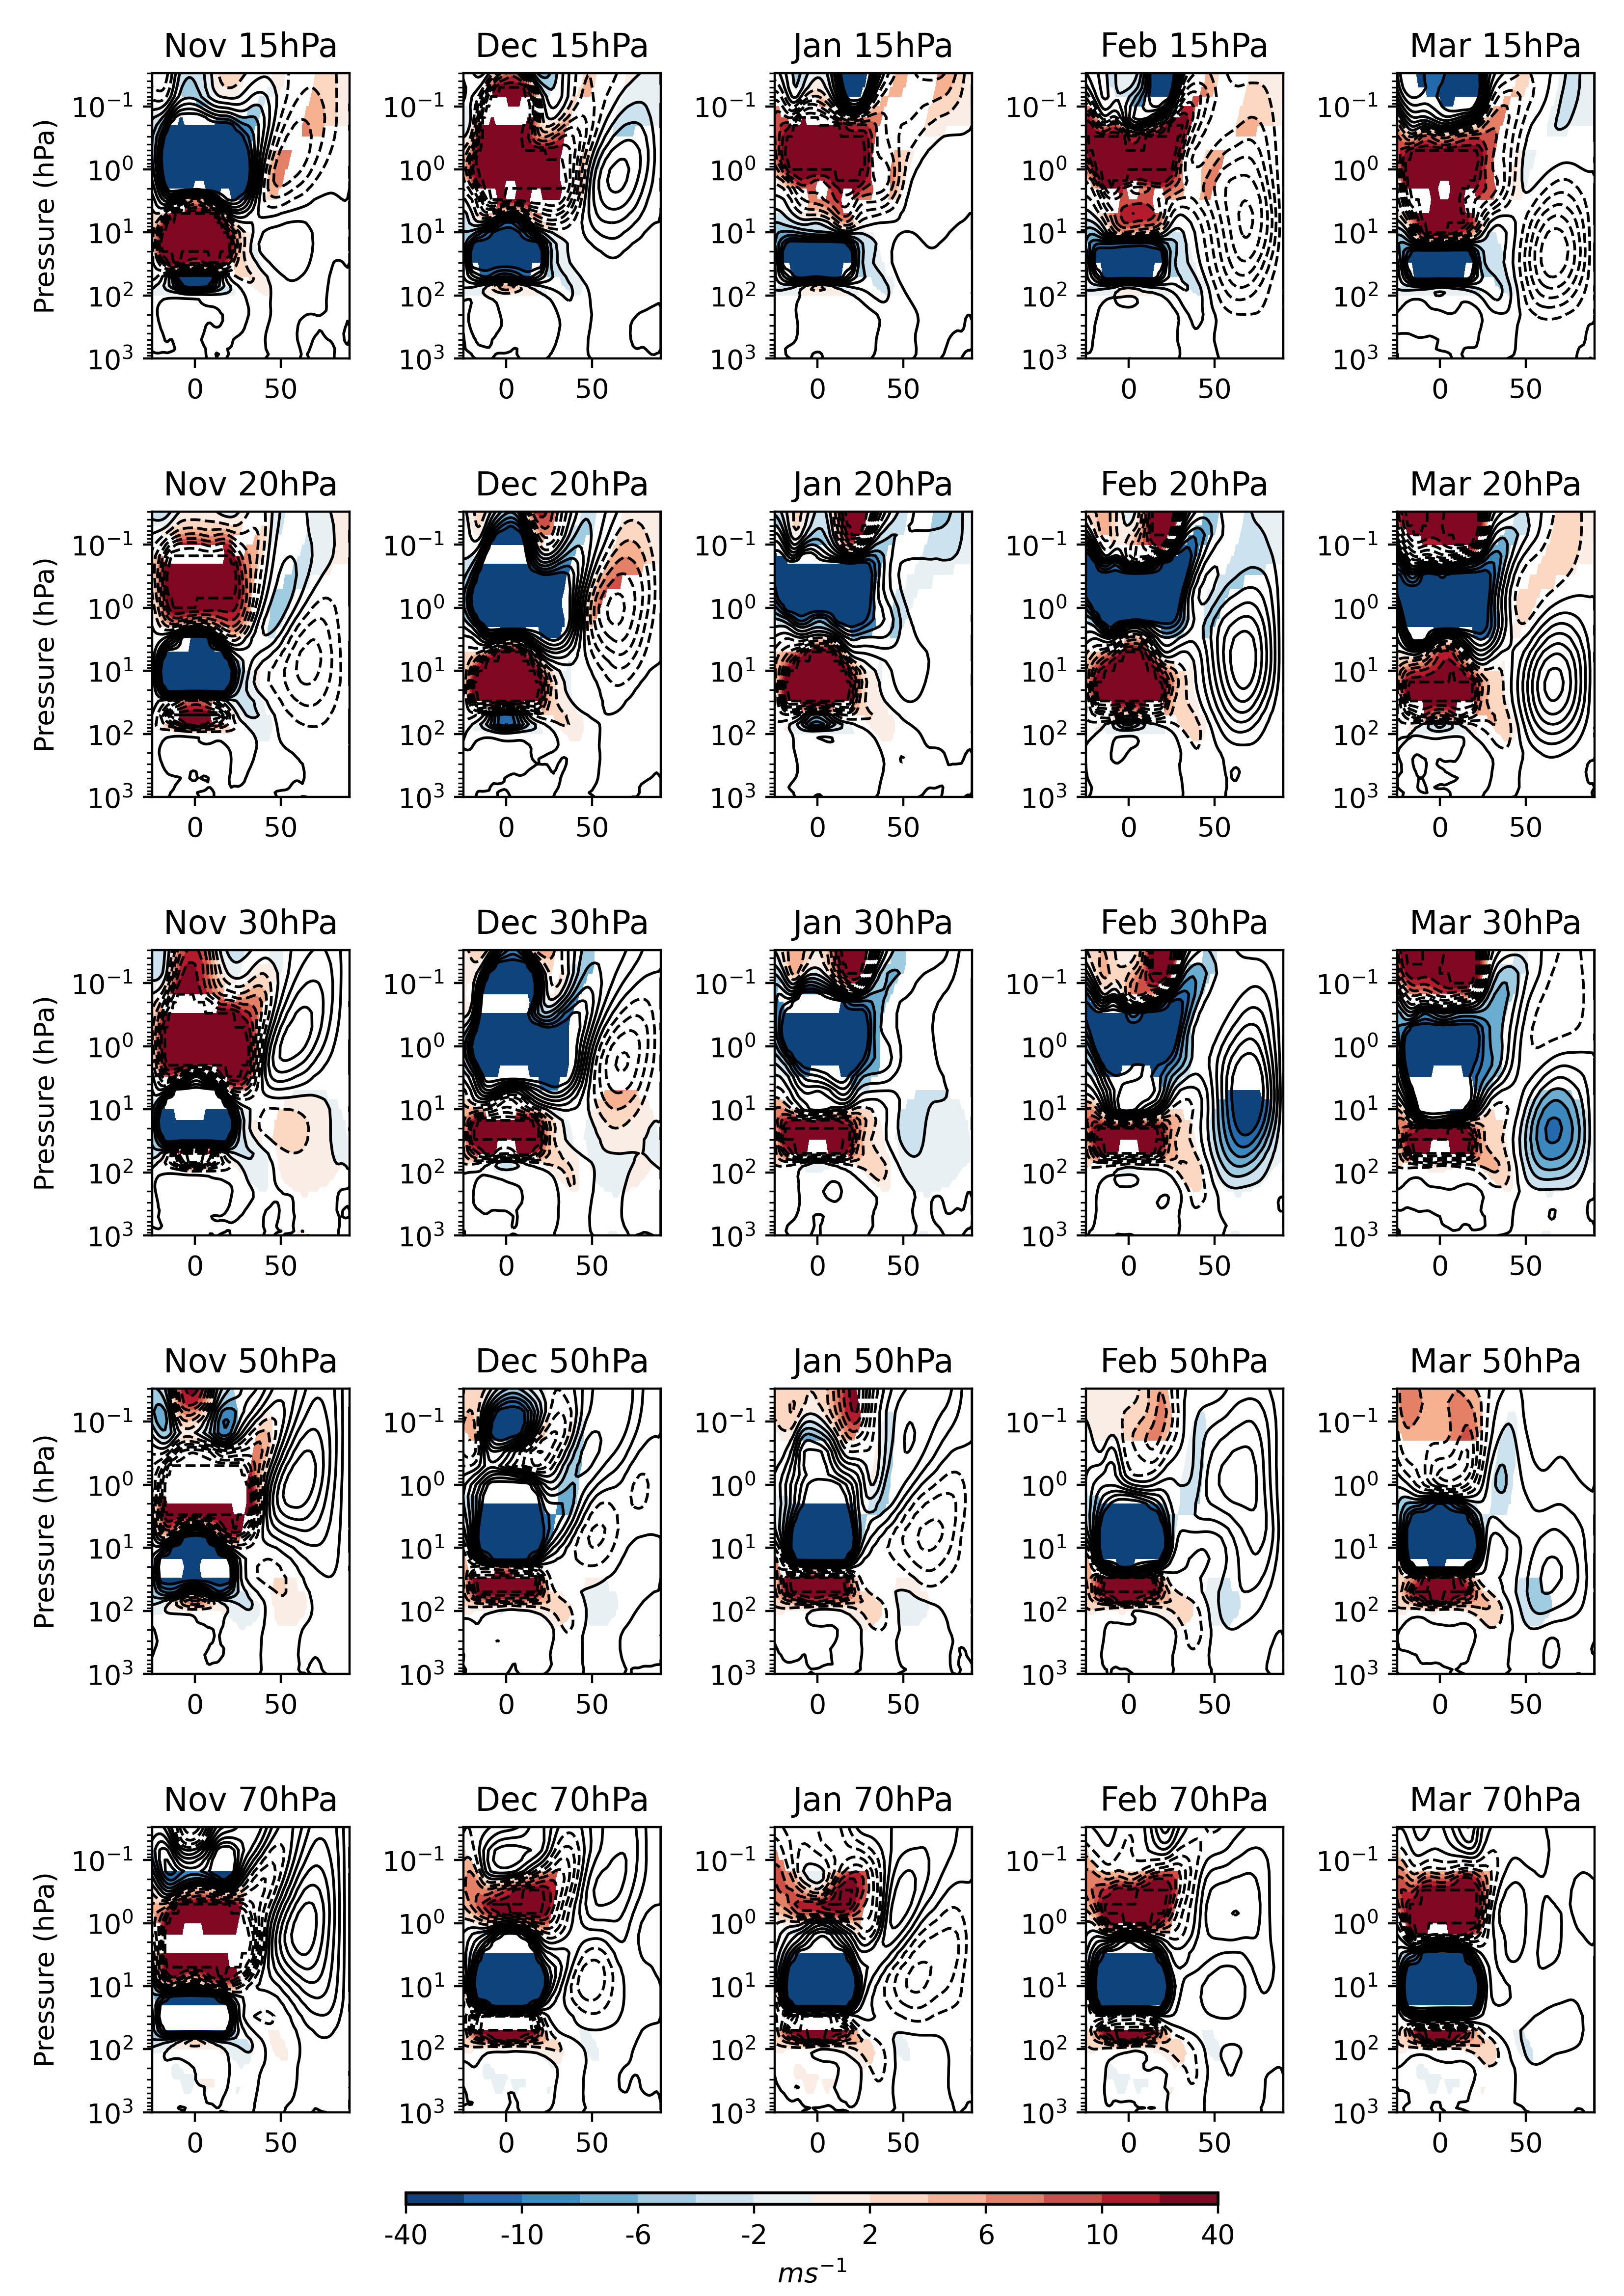
\includegraphics[width = 0.9\linewidth]{Figures/Figures-deepQBO/ZMZW_composites_by_month_QBO_phases_U_s_MarQBO_vs_Mar_70hPa_5thresh.png}
\caption[ZMZW composites under different QBO phases in the shallow QBO simulation]{Like figure \ref{fig:HT_piclim} for the shallow QBO experiment.}
\label{fig:HT_shallow}
\end{center}
\end{figure}
\newpage 

To examine these large mid-winter vortex responses in the deep simulation more closely, we analyse the responses of planetary wave propagation to different QBO phases. figure \ref{fig:EP_deep} shows composites of meridional and vertical EP flux arrows and EP flux divergence under QBOE (top row) and QBOW conditions (middle row) as well as differences between the phases (bottom row) from the deep experiment. In addition, we include the zero wind line of ZMZW composites under QBO phases on figure \ref{fig:EP_deep} to examine the association between wind anomalies and the direction of wave propagation. 

The largest differences in EP flux are visible in January. In this month,
there is greater EP flux divergence (i.e. larger negative $\nabla \cdot F$) over the vortex region (near 60$^\circ$N on the 10 hPa level) for QBOW indicating increased wave driving of the vortex under this phase compared to QBOE. This indicates that under QBOE conditions, more planetary waves are permitted to propagate towards the equator and away from the vortex. This confirms that the HT link the mid-winter in the deep experiment is reversed compared to ERA-Interim. The precise causes for this reversal are as yet unexplained however, QBOE conditions are associated with enhanced equatorward EP flux propagation near 40$^\circ$N between the 1 hPa and 0.1 hPa levels compared to QBOW. In this same region, QBOW phases are associated with an arm of the easterly SAO phase which encroaches poleward into the extra-tropics near the 0.8 hPa level (indicated by the zero wind line on composites). The role that variability in this region may play in accounting for responses patterns to the QBO is explored in further detail in section \ref{sec:role_SAO}.
\newpage
\begin{figure}[h!]
\begin{center}
\noindent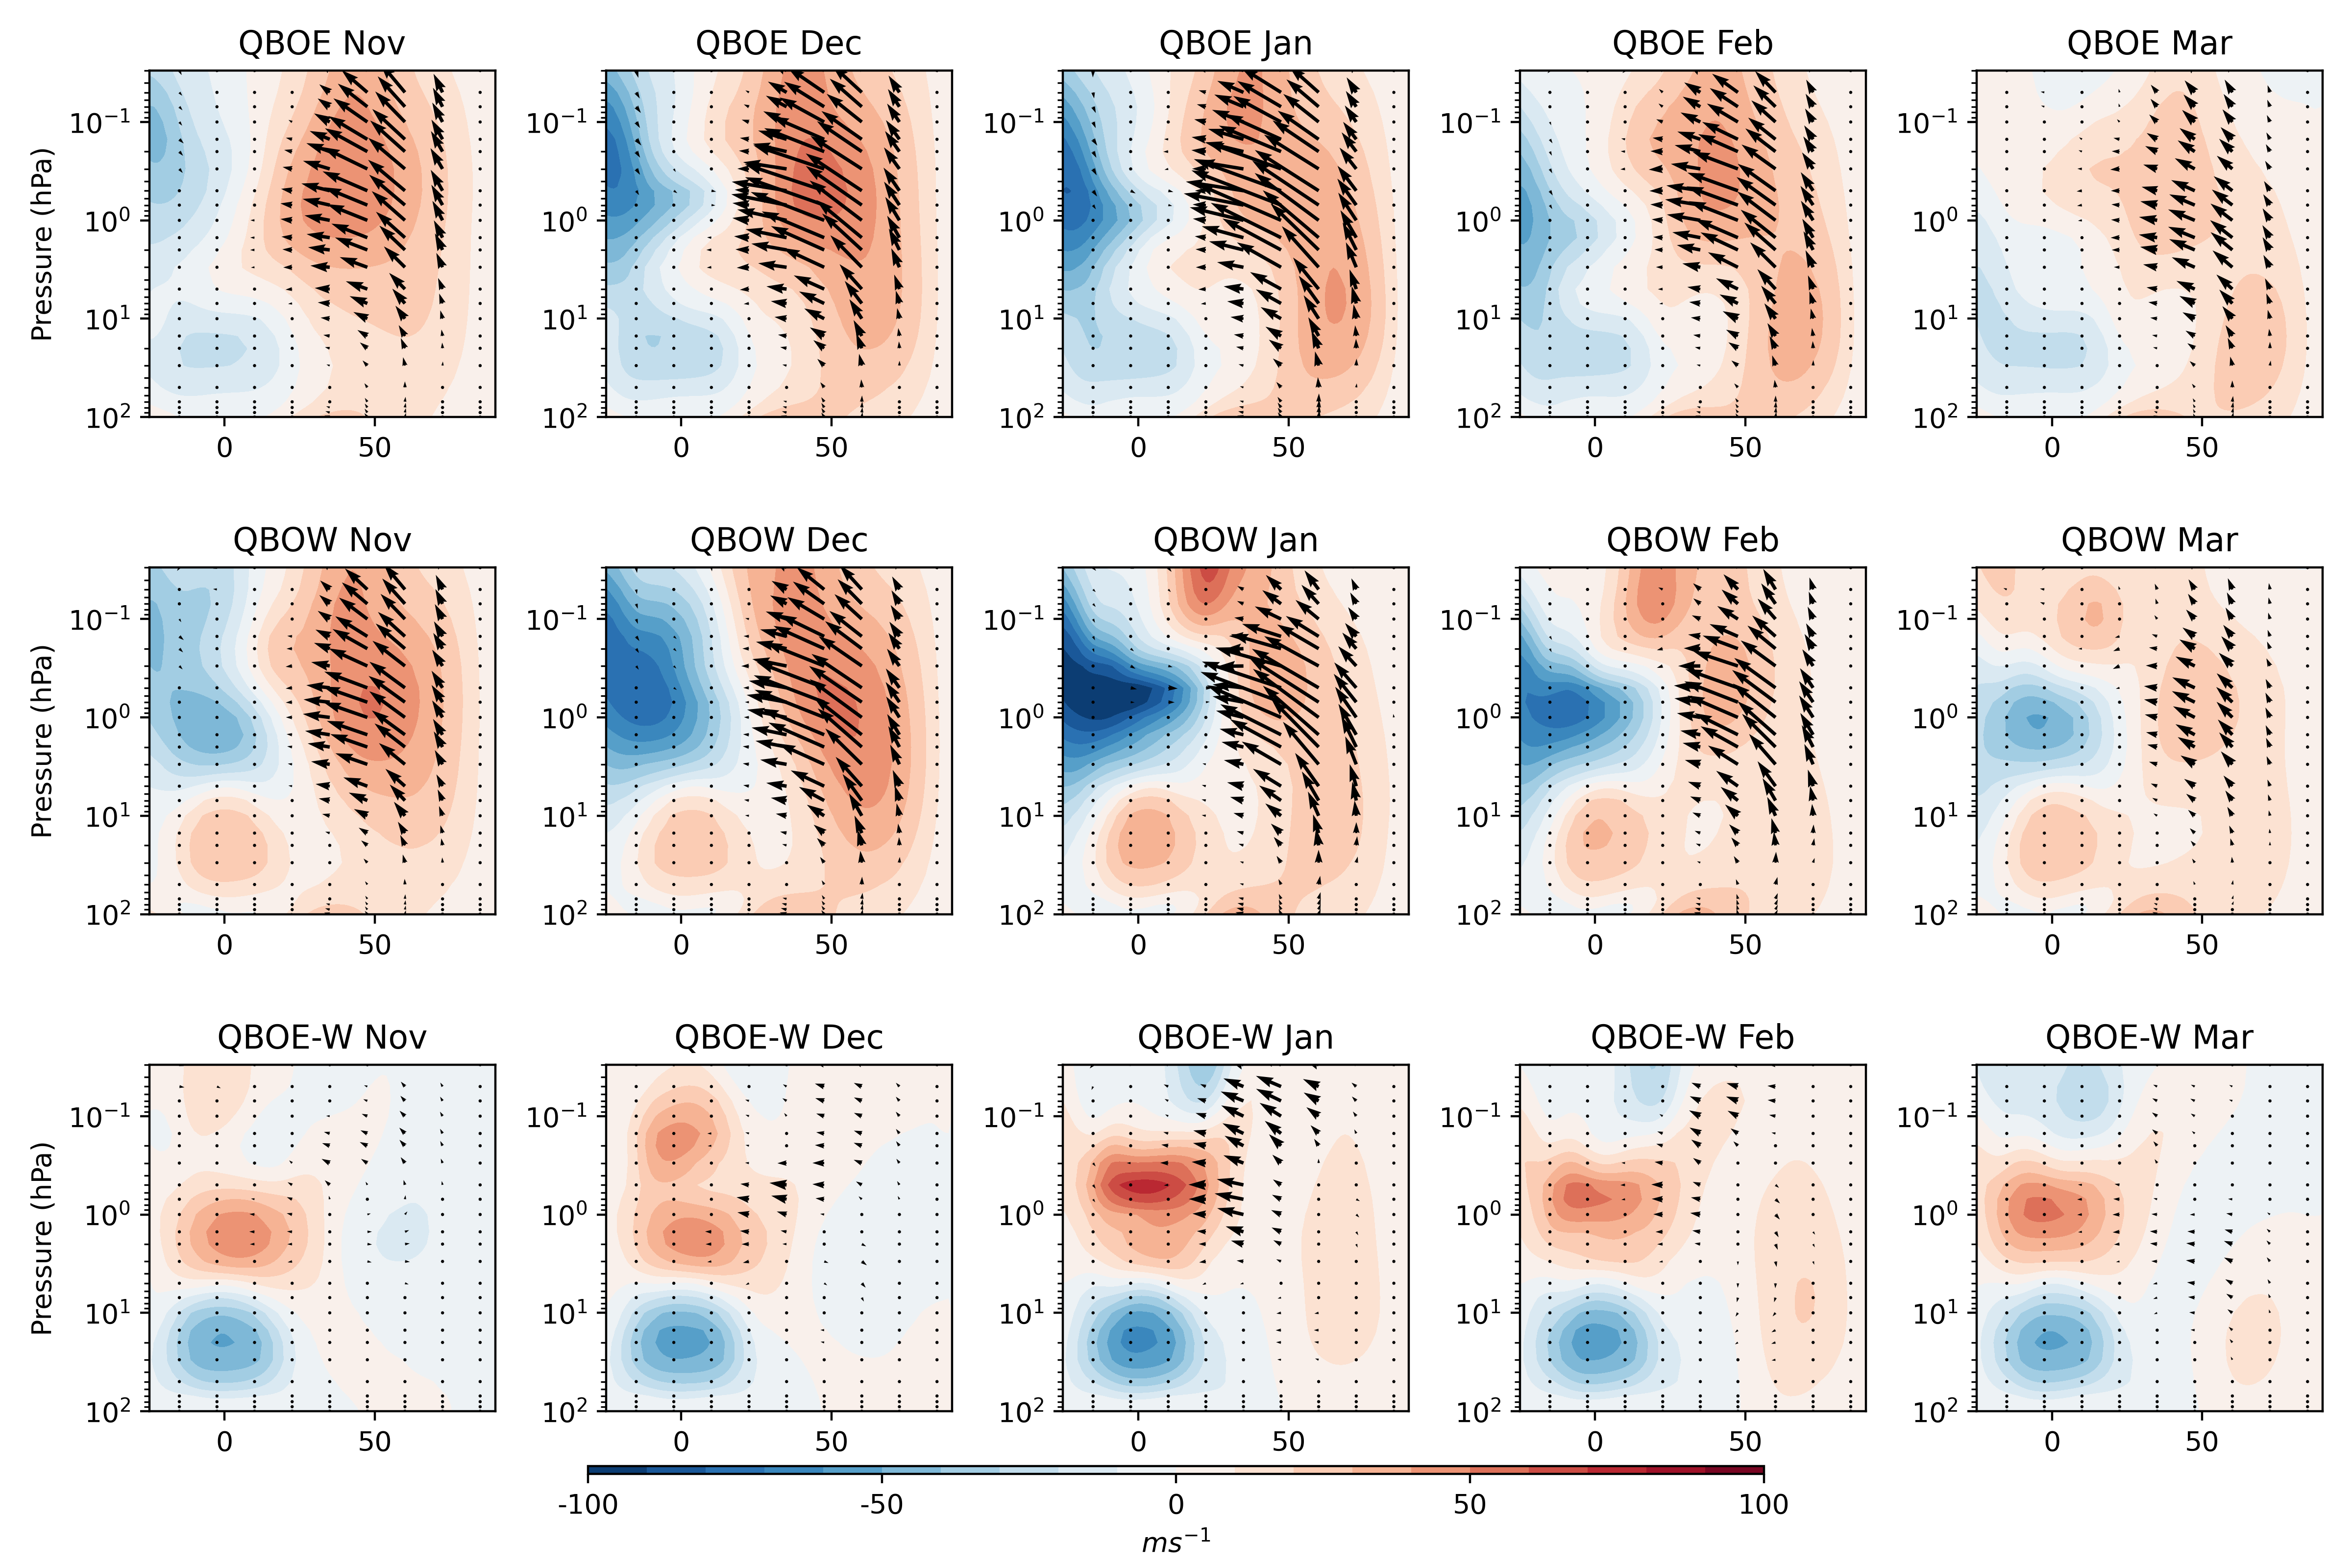
\includegraphics[width = \linewidth]{Figures/Figures-deepQBO/EP_flux_composites_by_month_QBO_phases_d_higher_50hPa_5thresh.png}
\caption[EP flux composites under different QBO phases in the deep QBO simulation]{Deep QBO experiment composites of EP flux divergence (coloured shading) and EP fluxes (arrows with units of $m^2s^{-2}$), which indicate the direction of wave propagation, under QBOE (top row) and QBOW (middle row) conditions as well as the difference between QBOE and QBOW composites (bottom row) for November-March. QBO phases are defined as any Nov-Dec equatorial winds which exceeds a magnitude of $5ms^{-1}$ on the 50 hPa level. Thick black lines denote the 0-wind line of ZMZW composites evaluated using the same QBO phases.}
\label{fig:EP_deep}
\end{center}
\end{figure}

Also evident in the ZMZW composites from the deep experiment (figure \ref{fig:HT_deep}) are elements of connection between the QBO and the surface: Between $\sim$45-55$\degree$N latitudes, a limb of anomalies associated with QBO phases descends into the troposphere (below 100 hPa) and to the surface. These anomalies are of the same sign as the QBO anomaly in the middle equatorial stratosphere and increases in magnitude as well as propagation towards the surface throughout the winter season with significant composite differences reaching the surface in February and March. This feature is not evident in the composites of the shallow experiment but is observed in the pi-clim cntrl albeit at a lower magnitude and only for a selection of months (February and March using a 30 hPa QBO, for example). This feature may be evidence in support of a subtropical pathway between the QBO and surface suggested in \cite{graySurface2018b} but, on the other hand, it is only ever present with significant vortex anomalies, so it may simply be a secondary response to the vortex anomaly involving a latitudinal shift of the mid-latitude jet (as in \cite{baldwinStratospheric2001a}). 

\section{The role of the SAO region}
\label{sec:role_SAO}

ZMZW composites in figure \ref{fig:HT_deep} show positive (negative) vortex responses to QBOE (QBOW) conditions in late winter which are significantly enhanced in the deep experiment. They are also consistent with enhanced late winter MSLP responses in the deep experiment (figure \ref{fig:SLP_deep}) which are opposite to those seen in the observations \cite{graySurface2018b} and in earlier experiments \cite{andrewsObserved2019d}. However, the cause of these responses in the vortex are as yet unclear. 

A prominent feature of the ZMZW composites in the deep simulation (figure \ref{fig:HT_deep}) is the presence of anomalies in the SAO region (above the 1 hPa level): Composite differences in the upper equatorial stratosphere in this experiment exhibit large anomalies of the opposite sign to the QBO phase below. These anomalies are evident throughout NH winter season and are not sensitive to the choice of QBO level. This is consistent with the idea of vertically coherent QBO phases filtering out waves with the same phase speed direction as the QBO by preventing propagation through the QBO region according to the Charney-Drazin Criteria. Conversely, wave forcing of the opposite phase speed of the deep QBO is permitted to propagate into the lower mesosphere where momentum is transferred to the mean flow leading to SAO anomalies of the opposite sign to the QBO. 

This modulation of the SAO by the QBO can be further demonstrated by examining a time series of deseasonalised equatorial ZMZW anomalies in each simulation (figure \ref{fig:experiment_QBOs_anomalies}). Once the seasonal cycle in SAO winds is removed, both the deep and shallow QBO variations (sub-figures a and c) are seen to extend beyond the nudging region up to near the 0.1 hPa level. This is also reflected in the Fourier power spectra (figures \ref{fig:experiment_QBOs_anomalies}b and d) which show significant power corresponding to the QBO period up into the mesosphere, an effect reported in \cite{kuaiNonstationary2009c} who show elements of synchronisation between the QBO and SAO. QBO signals in the SAO region are less prominent in the pi-clim cntrl and ERA-Interim winds (figures \ref{fig:experiment_QBOs_anomalies}e-h) with QBO variations extending to approximately the 1 hPa level in the Fourier spectra. 

\begin{figure}[h!]
\begin{center}
\noindent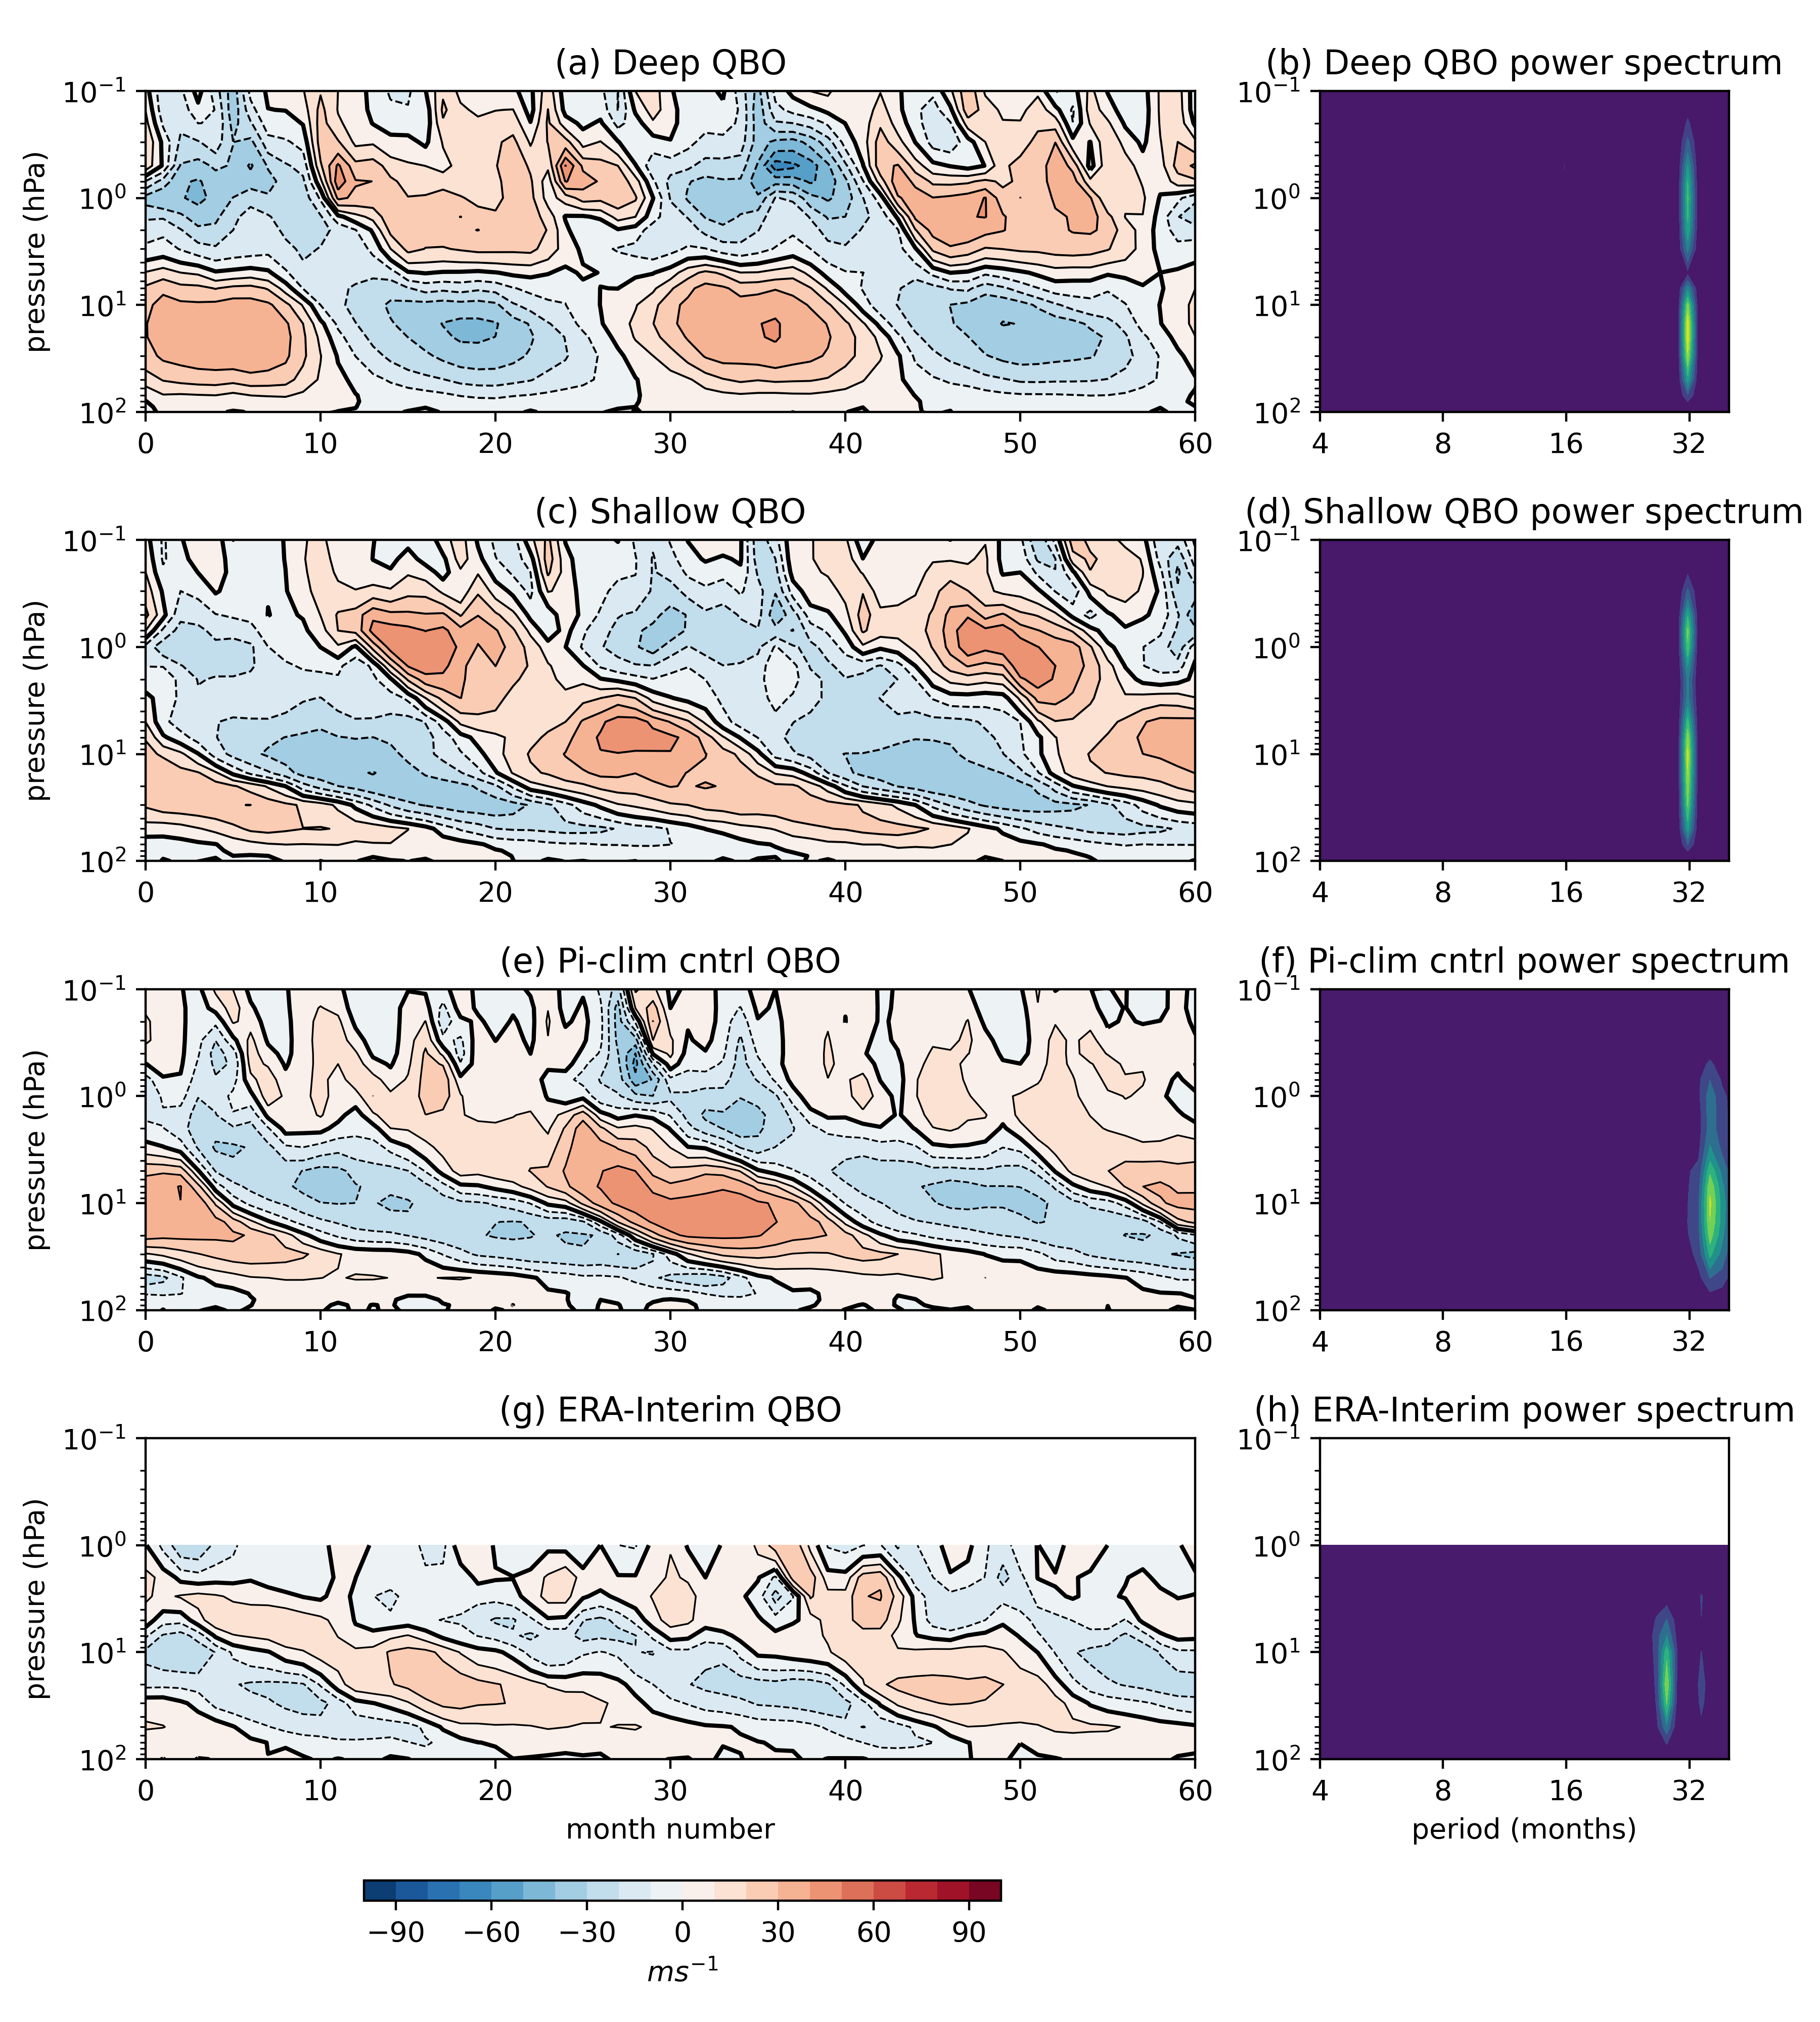
\includegraphics[width = 0.75\linewidth]{Figures/Figures-deepQBO/experiment_QBOs_anomalies.png}
\caption[Equatorial ZMZW anomaly time-height profiles from QBO experiments]{5 year sample of deseasonalised ZMZW anomalies averaged between 5$^{\circ}$\,S--5$^{\circ}$\,N latitude from the deep QBO (a), shallow QBO (c) and pi-clim cntrl (e) simulations and ERA-Interim (g). Thick black contours denote the 0-wind line where westerlies meet easterlies. Sub-figures b, d, f and h show Fourier Power spectra for equatorial wind anomalies at various levels from the same datasets.}
\label{fig:experiment_QBOs_anomalies}
\end{center}
\end{figure}

There are also significant extra-tropical ZMZW anomalies associated with these QBO-like variations in the upper stratosphere/lower mesosphere (USLM) region. Figure \ref{fig:SAO_comp_1hPa} show ZMZW composite differences between USLM QBOE and USLM QBOW conditions defined using extremes in the deseasonalised winds on the 1 hPa level (to remove the effect of the seasonal cycle). The largest responses in the vortex region are apparent in the deep experiment (figure \ref{fig:SAO_comp_1hPa}, top row). In mid-late winter, large anomalies are apparent near 60$\degree$N for USLM QBOE - QBOW composite differences. These responses correspond to a weakened (strengthened) vortex for USLM QBOE (QBOW) anomalies. In the equatorial region, large USLM anomalies are evident near the 1 hPa level (resulting from the design of the composites). These USLM anomalies also significantly encroach into the extra-tropical region with significant composite differences apparent out to latitudes of $\sim$45$\degree$N. Between 100 hPa and 10 hPa, significant QBO anomalies are evident of the opposite sign to those in the USLM region above. This provides further evidence of the mechanisms described above by which the QBO and SAO co-vary significantly. The vortex responses to the USLM QBO in the other experiments are significantly smaller than the corresponding responses in the deep QBO simulation - negative vortex composite differences are only evident in late winter (Feb-Mar) in the shallow simulation (figure \ref{fig:SAO_comp_1hPa}, middle row) and there are no vortex responses deemed significant under a student's t-test in the pi-clim cntrl (bottom row). Composite differences in the equatorial USLM region in these experiments are also more confined to the equatorial region than those in the deep experiment. These composites indicate that variability in the SAO region may play a key role in modulating vortex strength, particularly in the deep experiment which exhibits larger and more widespread USLM anomalies than the other two experiments.
\newpage
\begin{figure}[h!]
\begin{center}
\noindent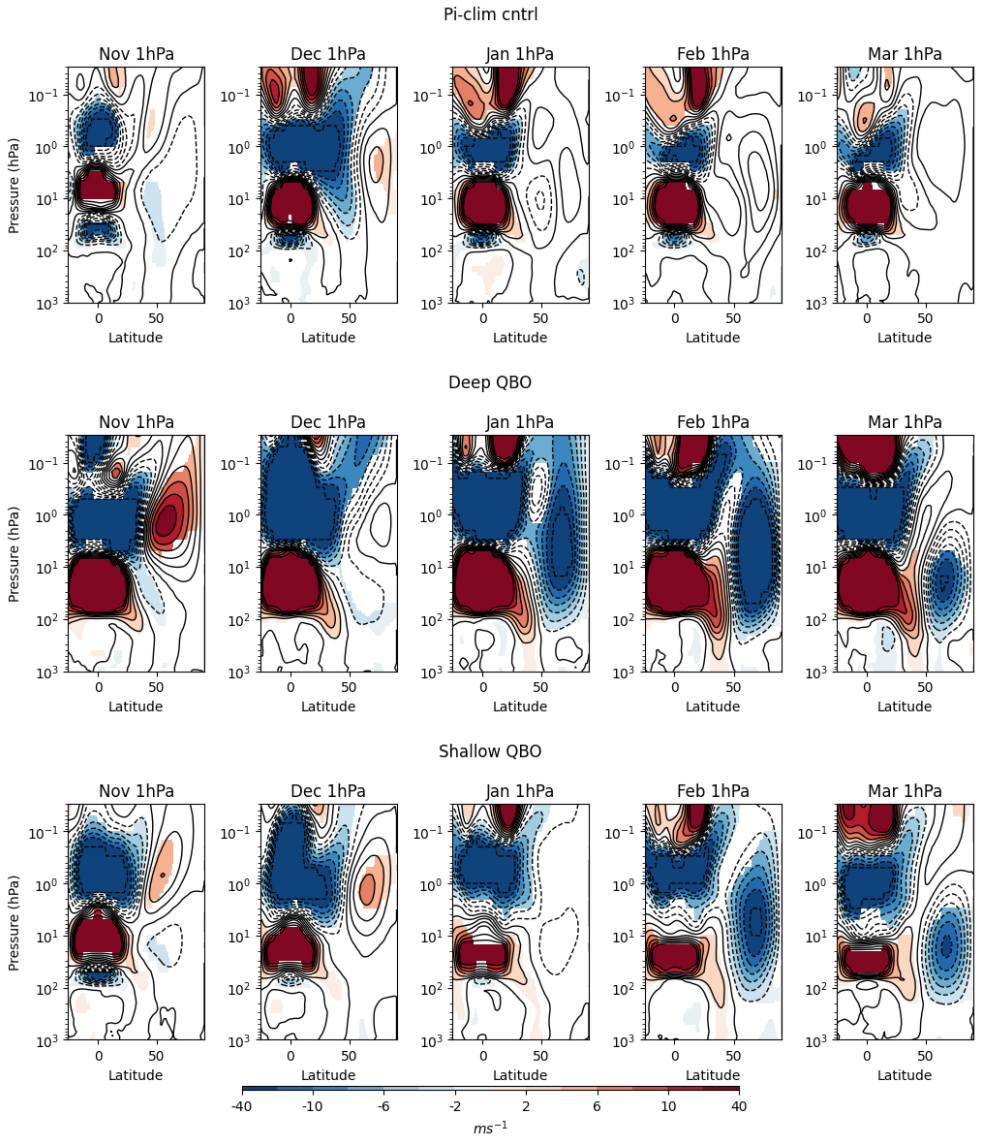
\includegraphics[width = 0.8\linewidth]{Figures/Figures-deepQBO/SAO_composites_combined.png}
\caption[ZMZW composites under easterly and westerly SAO anomalies]{ZMZW composite differences between anomalous easterly and westerly SAO conditions from the deep QBO (top row), shallow QBO (middle row) and pi-clim cntrl (bottom row) simulations. An SAO anomaly is defined as any deseasonalised Nov-Dec monthly equatorial ($5^{\circ}$\ S--$5^{\circ}\ $N average) ZMZW that exceeds a magnitude of 5 $ms^{-1}$ on the 1 hPa level. Lagged composite differences are evaluated in a range of NH winter months (indicated in sub-figure titles) based on anomalous SAO conditions. Coloured shading indicates ZMZW differences significant above the 95\% confidence level under a 2 tail student’s t-test.}
\label{fig:SAO_comp_1hPa}
\end{center}
\end{figure}


%----- EP flux fig description here -------

\cite{grayForecasting2020a} show a similar association between the SAO region and the vortex using a set of nudging experiments and suggest a connection via modulation of planetary wave propagation by SAO variations. To verify whether this mechanism may apply in the deep experiment (the simulation which exhibits the largest vortex responses to the equatorial USLM region) we analyse EP flux patterns associated with under different extremes in the USLM QBO. Figure \ref{fig:EP_deep_SAO} shows composites of EP flux arrows and divergence under USLM QBOE, USLM QBOW and USLM QBOE-QBOW. The EP flux divergence composite patterns are of the opposite sign to those associated with the QBO in the middle stratosphere (figure \ref{fig:EP_deep}) with greater flux divergence (i.e. larger negative $\nabla \cdot F$) over the vortex region under QBOE in January and February. The composites in these months are characterised by enhanced pole-wards propagation of extra-tropical EP flux arrows between the 1 hPa and 0.1 hPa levels under USLM QBOE as well as an encroachment of the summer easterlies near the 1 hPa level, denoted by the zero-wind line on figure \ref{EP_deep_SAO}, into the NH extra-tropics also under this phase. These are the opposite to patterns associated with the 50 hPa QBO which indicates enhanced equatorwards flux on the same levels under QBOE. These composites indicate that under USLM QBOE (QBOW) conditions, mid-latitude waves are directed from the extra-tropics towards (away from) the vortex leading to increased (decreased) wave driving of the vortex and a subsequent weakening (strengthening) of vortex winds.

%----- EP flux fig description here -------

\begin{figure}[h!]
\begin{center}
\noindent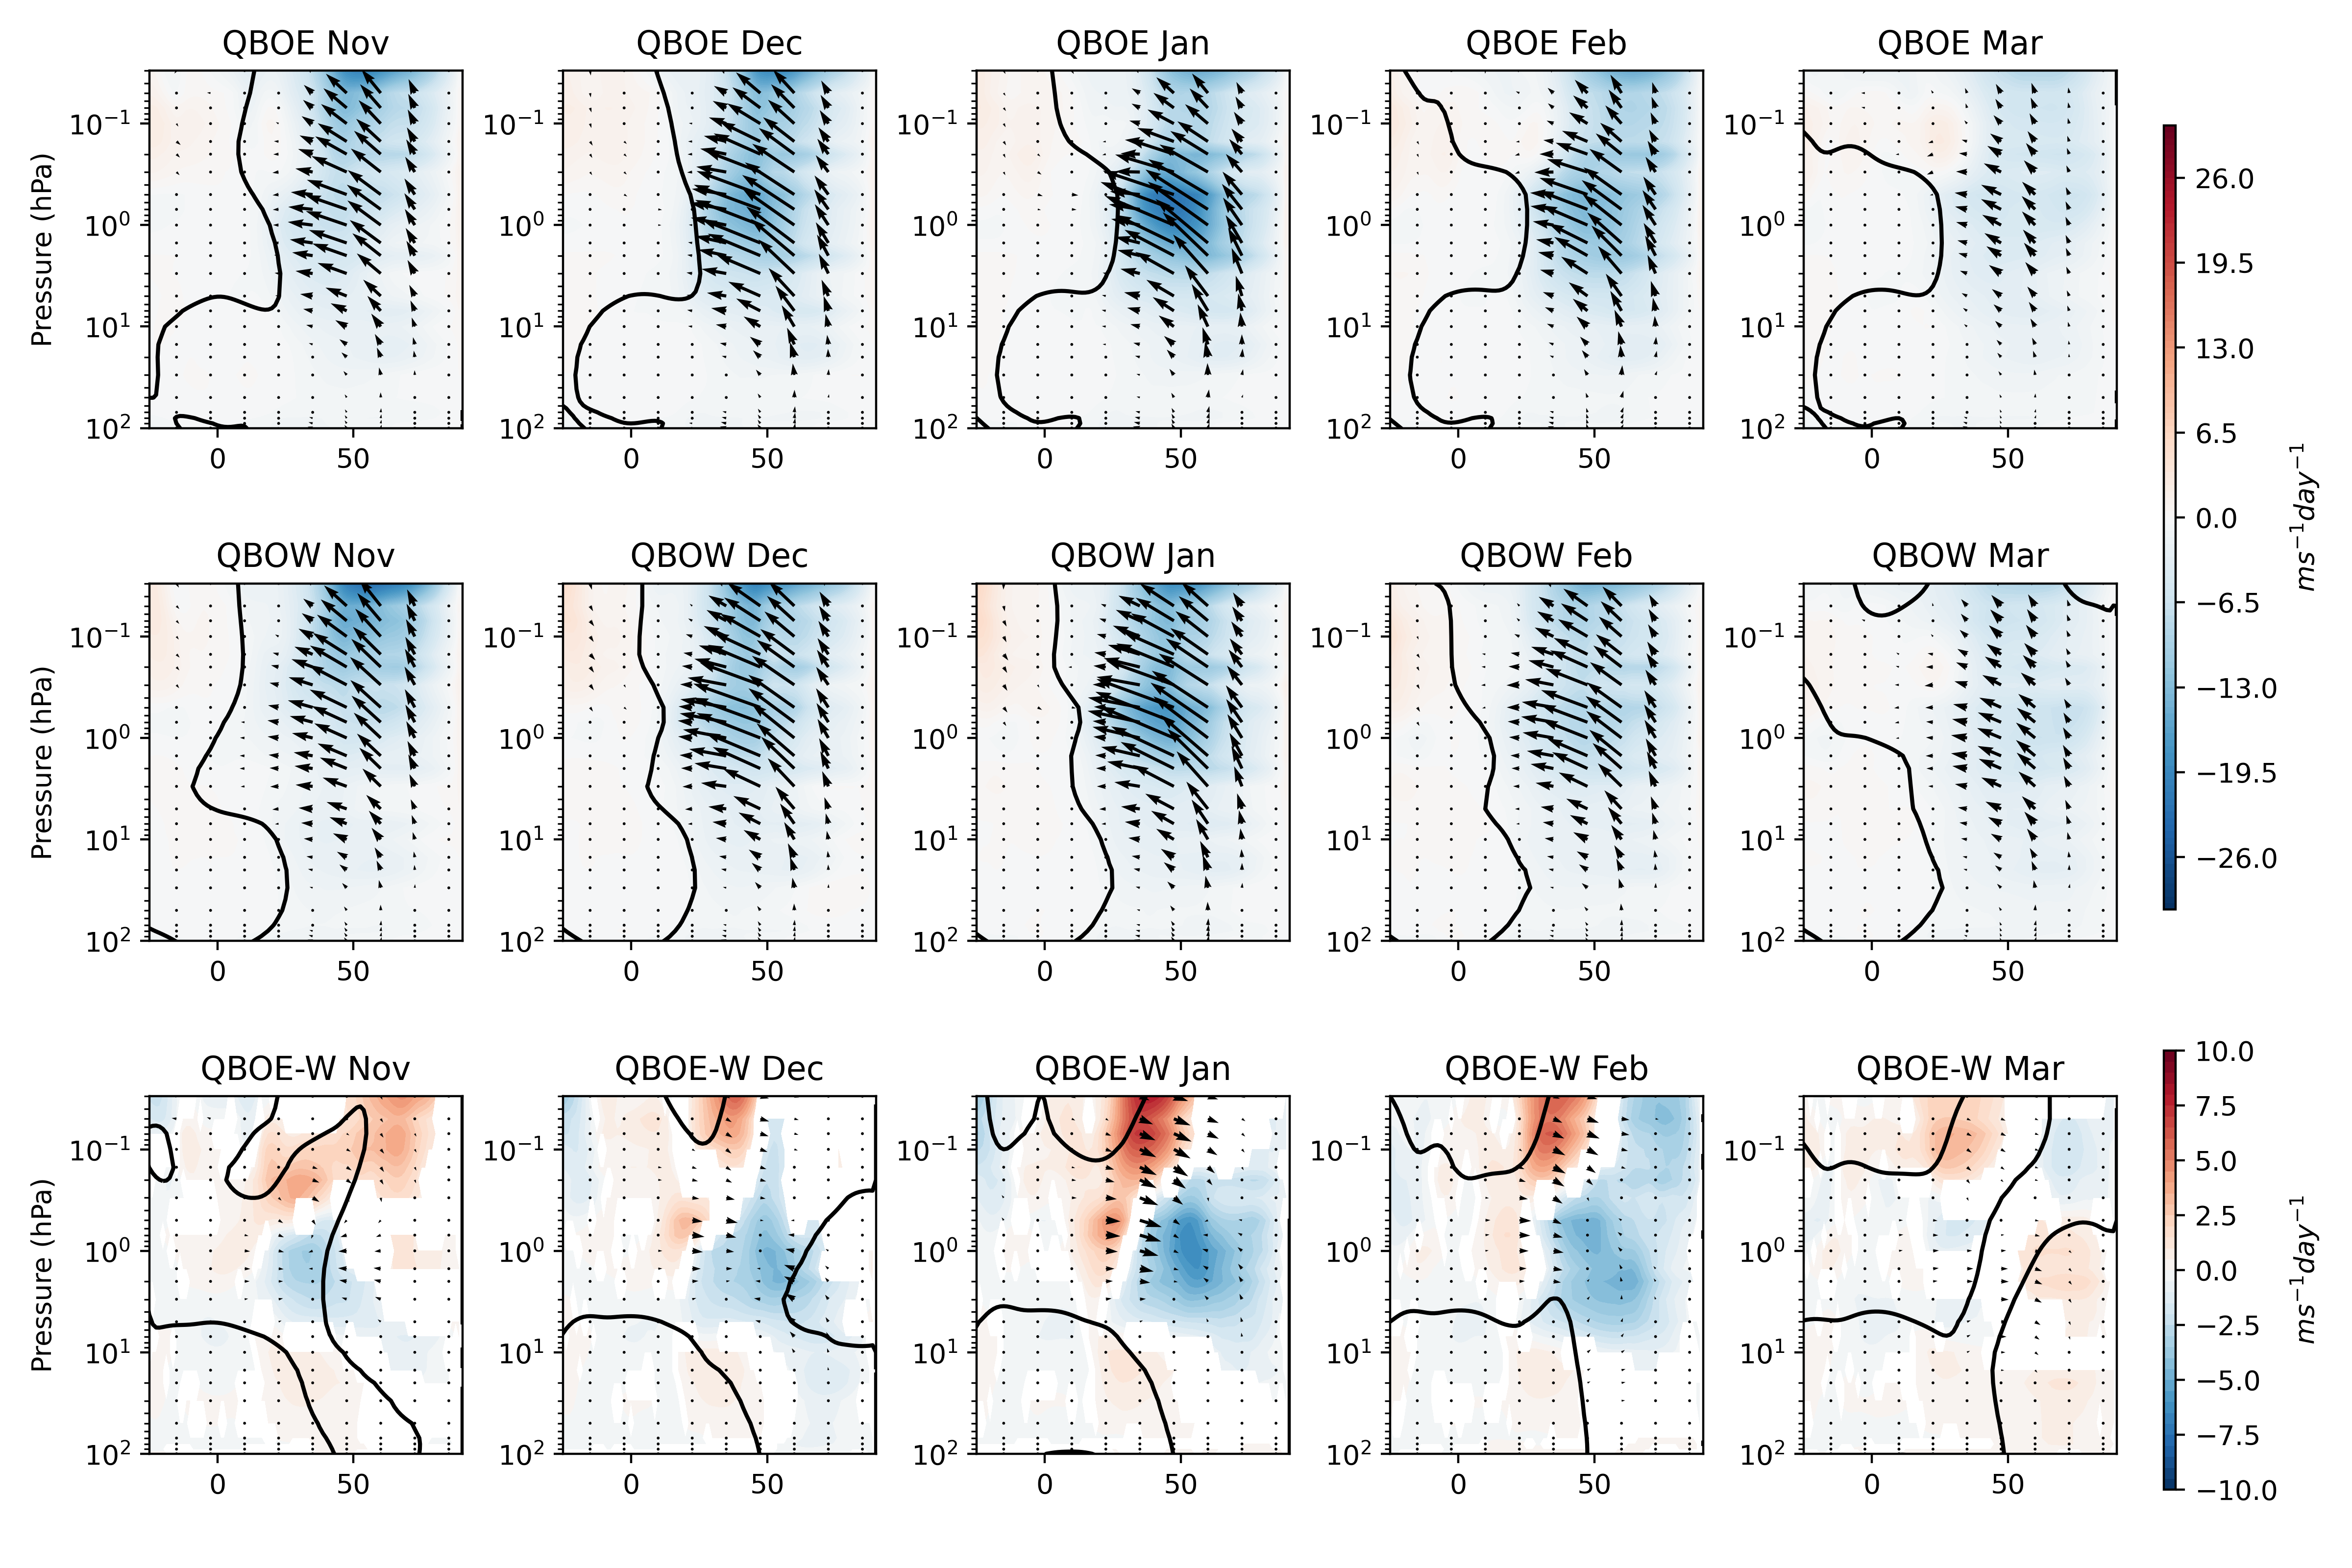
\includegraphics[width = \linewidth]{Figures/Figures-deepQBO/EP_flux_composites_by_month_QBO_phases_d_higher_anom_1hPa_5thresh.png}
\caption[EP flux composites under different USLM QBO phases in the deep QBO simulation]{Deep QBO experiment composites of EP flux divergence (coloured shading) and EP fluxes (arrows with units of $m^2s^{-2}$), which indicate the direction of wave propagation, under USLM QBOE (top row) and USLM QBOW (middle row) conditions as well as the difference between QBOE and QBOW composites (bottom row) for November-March. QBO phases are defined as any deseasonalised Nov-Dec equatorial wind anomaly which exceeds a magnitude of $5ms^{-1}$ on the 1 hPa level. Thick black lines denote the 0-wind line of ZMZW composites evaluated using the same USLM QBO phases.}
\label{fig:EP_deep_SAO}
\end{center}
\end{figure}

Combining the results from this section provides a potential mechanism by which the equatorial USLM modulates the later winter vortex response to mid-stratosphere QBO phases in the deep experiment (as seen in composites in figure \ref{fig:HT_deep}): The design of the deep QBO experiment has resulted in an unexpectedly strong modulation of the equatorial USLM region, through the filtering of equatorial waves as they propagate vertically through the deep QBO region. As a result, there is a two-fold vertical structure in the equatorial ZMZW QBO anomaly, with a strong westerly (easterly) bias in the USLM overlying the QBOE (QBOW) anomaly in the lower stratosphere. This, in turn, permits more (less) equatorwards propagation of mid-latitude planetary waves in the upper stratosphere leading to reduced (increased) wave driving of the vortex and a subsequent strengthening (weakening) of the vortex. It thus appears that, in this experiment, the influence from QBO variations in the equatorial USLM overwhelm the influence from the QBO variations in the lower stratosphere.  Finally, these vortex anomalies (that are of opposite sign to the traditional HT relationship) propagate to the surface and result in the MSLP response patterns to QBO phases in figure \ref{fig:SLP_deep} thus explaining the incorrect sign of the MSLP anomalies when compared to the observed response. On the other hand, however, anomalies in the equatorial USLM may also be in response to the vortex anomalies - i.e. the vortex may respond to QBO phases and subsequently modulate the direction of EP flux equatorwards leading to USLM anomalies associated with different mid-stratosphere QBO phases. This complex interplay of potential mechanisms makes it difficult to definitively explain the responses to the QBO in our deep experiment. 

\section{Results in the context of previous work}
Our analysis so far indicates that a perpetually deep QBO leads to large responses in the vortex and NH MSLP of the opposite sign to a HT link as well as those shown by previous work \citep{andrewsObserved2019d} and that variability in the USLM region may be key to modulating this response. \cite{andrewsObserved2019d} did not study the HT relationship or other atmospheric responses to the QBO explicitly but showed an enhanced MSLP response consistent with a HT link (i.e. QBOE phase associated with a negative NAO pattern) using a deep QBO metric in both reanalysis and a free-running model. Accounting for the discrepancy in responses between our experiments and those of \cite{andrewsObserved2019d} may be key to understanding the mechanisms involved in QBO teleconnections but requires closer examination of the stratospheric responses in their model simulation.

An analogous measure of the effect of a deep QBO metric to that in \cite{andrewsObserved2019d} is to analyse the UKESM pi-control simulation utilised in chapters 3 and 4. Indeed, \cite{andrewsObserved2019d} use the HadGEM3-GC2 model \citep{williamsMet2018b}, a predecessor of UKESM1, and the length of the pi-control (1000 years) allows for robust composite analysis. Figure \ref{fig:SLP_picontrol_50} shows MSLP composites for different QBO conditions using a QBO metric at 50 hPa, a standard level which also shows significant vortex responses from previous analysis (see figure \ref{fig:holton_tan_comp}), from the pi-control simulation. These composites show that this model does not exhibit coherent MSLP anomaly patterns over the Atlantic - there is little to no response in this region to either phase and marginal composite differences which peak in magnitude at $\sim$1.5 hPa compared to $\sim3.5$ hPa in the same region from ERA-Interim \citep{andrewsObserved2019d}. A significant Pacific response is evident in January which peaks in magnitude at $\sim$2 hPa composite difference, a similar magnitude to that in ERA-Interim also shown in \cite{andrewsObserved2019d}. The sign of this Pacific anomaly is consistent with that found in \cite{graySurface2018b} with QBOE(W) associated with positive MSLP anomalies \footnote{There is an asymmetry in the abundance of QBOE and QBOW months that make up the composites - Significantly more QBOE phases are observed in NH winter which is consistent with similar composite analysis in chapter 3 (figure \ref{fig:SSW_hist_QBO_phase}) in which this feature is discussed further.}.

\begin{figure}[h!]
\begin{center}
\noindent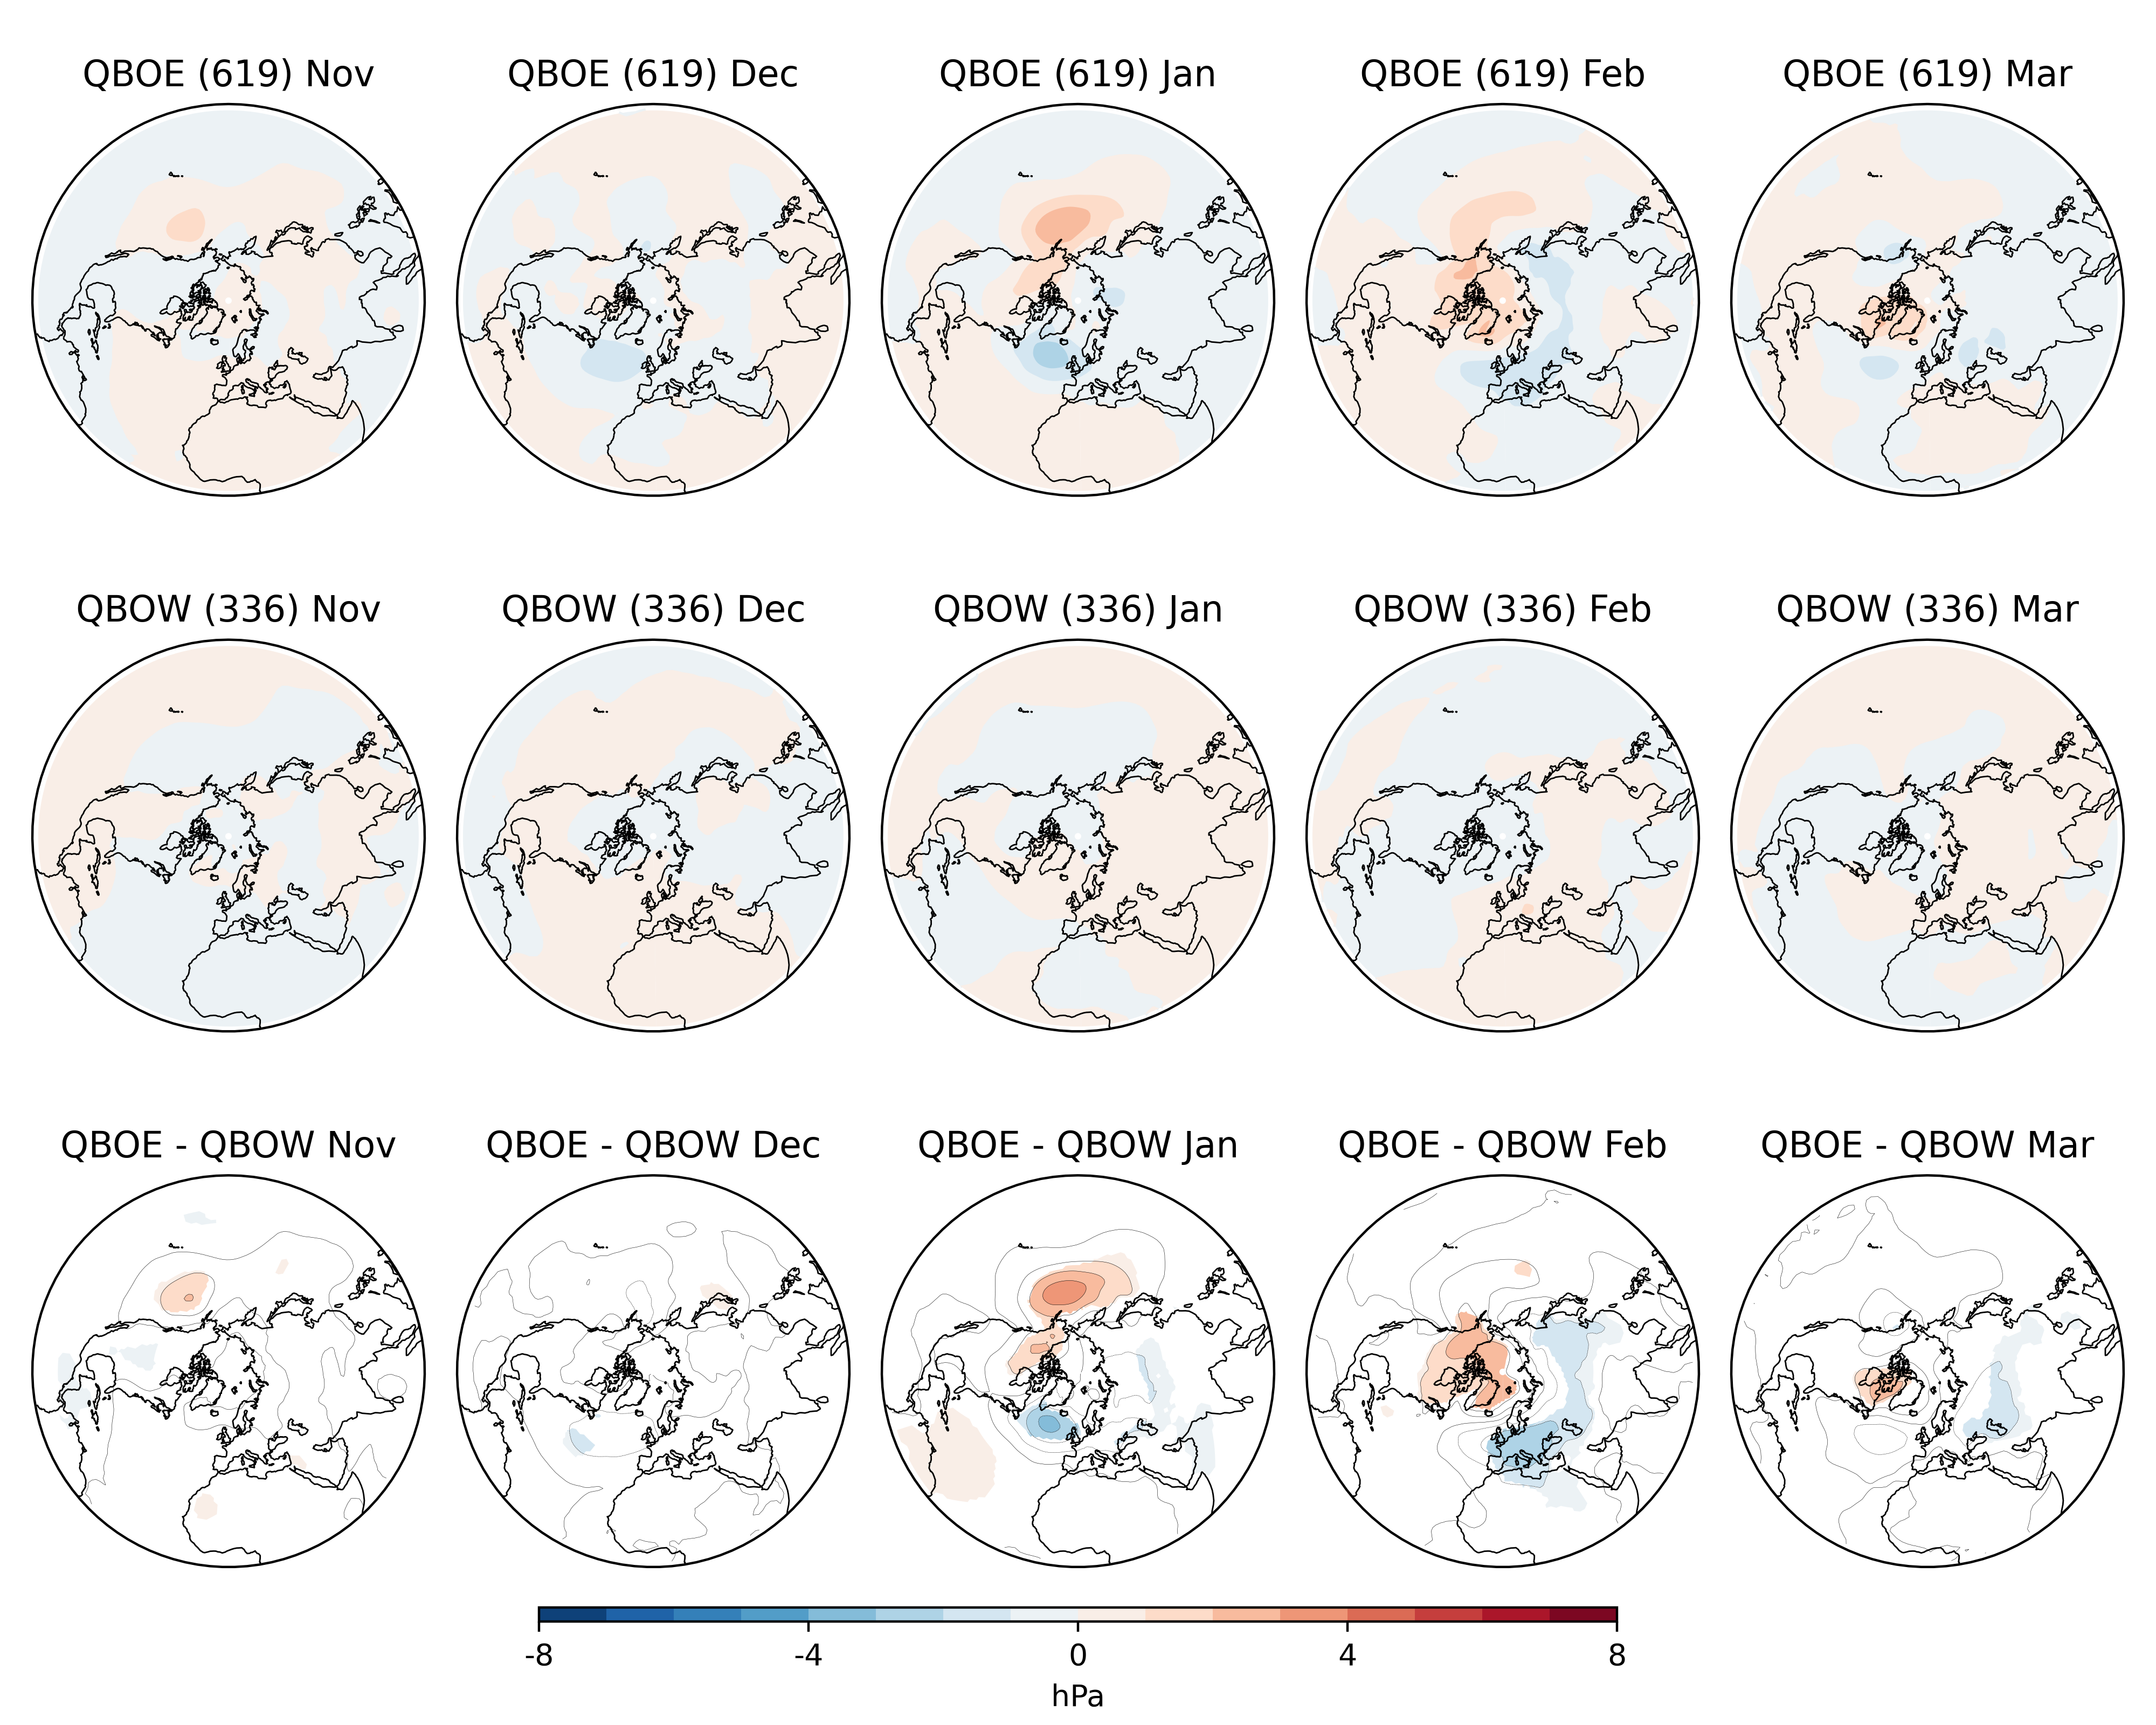
\includegraphics[width = 0.8\linewidth]{Figures/Figures-deepQBO/LAGGED_SLP_composites_individual_months_QBO_phases_U_picontrol_50hPa_5thresh.png}
\caption[MSLP composites under different 50 hPa QBO phases in the pi-control simulation]{like figure \ref{fig:SLP_piclim} for the pi-control simulation. QBO phases for each composite are defined as any monthly equatorial ($5^{\circ}$\ S--$5^{\circ}\ $N average) ZMZW that exceeds a magnitude of 5\ m\,s$^{-1}$ on the 50 hPa level.}
\label{fig:SLP_picontrol_50}
\end{center}
\end{figure}

We compare this single level definition to an analogous plot using a deep QBO metric. Figure \ref{fig:SLP_picontrol_deep} shows the MSLP composites when the QBO phase is defined using the deep QBO definition of \cite{andrewsObserved2019d}, i.e. by taking the average of the winds between 15-30 hPa instead of the single 50 hPa level. Anomalies associated with each phase of this deep metric are significantly enhanced compared to figure \ref{fig:SLP_picontrol_50}: Clear negative anomalies are visible over the northern node of the NAO (in the Icelandic region) for QBOW conditions peaking in January and similar anomalies are also apparent in February. There is also a coherent response to the deep QBO in the north Pacific which is first evident in December and increases in magnitude until a peak in February. The structure of this anomaly is distinct to that shown when using the 50 hPa QBO - under QBOW, a north-south dipole is evident with negative MSLP over the AL region and positive anomalies directly south of the Aleutian islands.

\begin{figure}[h!]
\begin{center}
\noindent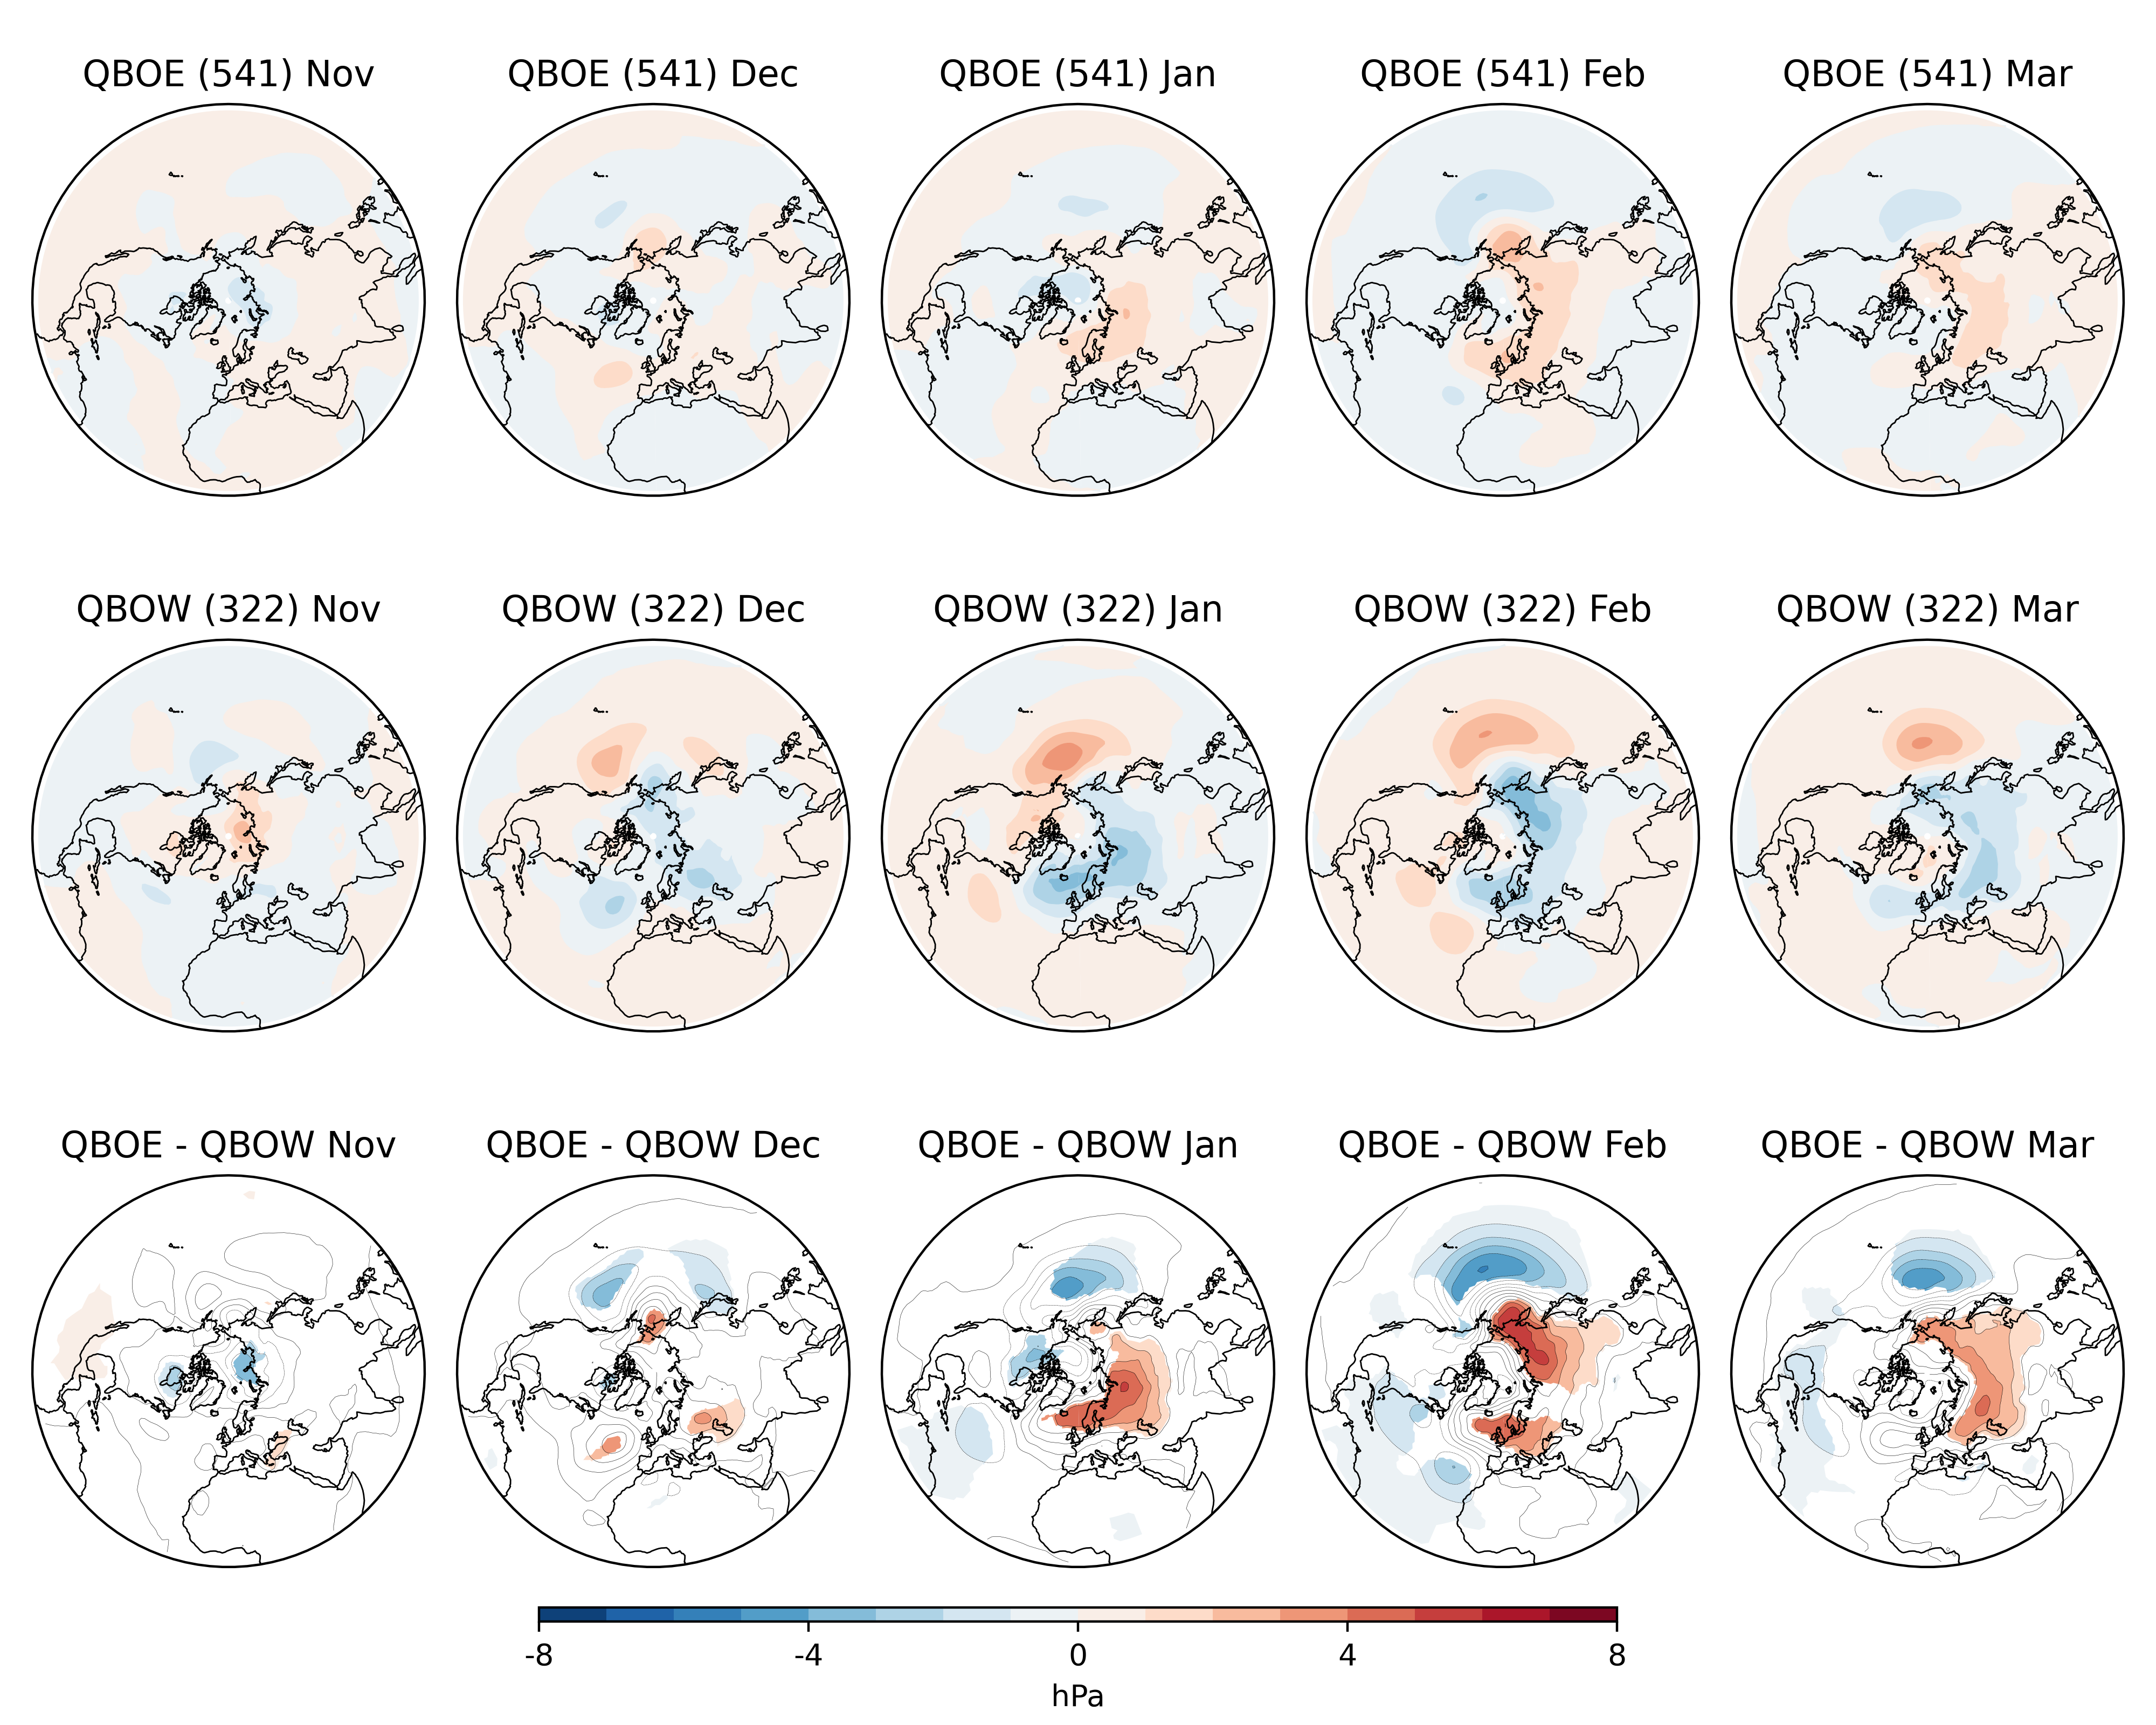
\includegraphics[width = 0.8\linewidth]{Figures/Figures-deepQBO/LAGGED_SLP_composites_individual_months_QBO_phases_U_picontrol_deephPa_1thresh.png}
\caption[MSLP composites under different deep QBO phases in the pi-control simulation]{Like figure \ref{fig:SLP_picontrol_50} but defining QBO phases using the same deep metric as employed in \cite{andrewsObserved2019d}, any monthly equatorial ($5^{\circ}$\ S--$5^{\circ}\ $N average) ZMZW averaged between the 15 hPa and 30 hPa levels that exceeds a magnitude of 5\ m\,s$^{-1}$.}
\label{fig:SLP_picontrol_deep}
\end{center}
\end{figure}

Importantly, the MSLP responses using the deep QBO metric are consistent with with the results of \cite{andrewsObserved2019d} (their figure 6). Namely, in the NAO region, the deep QBOE (QBOW) phase is associated with positive (negative) anomalies over the Icelandic low region and therefore a negative (positive) NAO. The structure of the Pacific responses is also consistent with their results; the QBOE (QBOW) phase is associated with decreased (increased) pressure over the AL region and increased (decreased) MSLP further south in the mid-Pacific. We can, therefore, confidently use this model simulation to extend the study of \cite{andrewsObserved2019d} by exploring whether the stronger MSLP response to a deep QBO definition is accompanied by a correspondingly stronger HT response in the stratosphere, or whether there is some other mechanism that comes into play. We can also examine the amplitude of the associated equatorial USLM anomaly and compare it with the large unusual two and three-fold structures seen in our deep QBO experiments (figure \ref{fig:HT_deep}), so that we can further understand the unexpected reversal of the MSLP response in that experiment.    

The pi-control also exhibits QBO-vortex coupling consistent with an expected HT effect - analysis from chapter 3 (figure \ref{fig:holton_tan_comp}) showed a negative composite difference in vortex winds for QBOE-QBOW conditions over the whole winter using both the single level (50 hPa) and deep QBO metrics. Interestingly, the magnitude of the high NH latitude response using the deep metric is similar to that exhibited for the 50 hPa QBO when measured over the whole season (figure \ref{fig:holton_tan_comp}). When the ZMZW composites from the pi-control are split up by month (figure \ref{fig:HT_picontrol}), the responses are also comparable in magnitude and both peak in January although anomalies associated with the deep metric are evident throughout the winter season while single level vortex responses are most evident in December and January.

A marked difference between these composites is the presence of a tropospheric sub-tropical anomaly using the deep metric which is present for all sampled months and absent when using the single level definition. This suggests that the enhanced MSLP responses using a deep QBO measure in the pi-control may arise via the subtropical pathway (which is absent using the 50 hPa QBO) in addition to a modulation of the high-latitude pathway via the HT link. Furthermore, the subtropical tropospheric anomalies are also present in the deep QBO experiment (figure \ref{fig:HT_deep}) and absent in the shallow simulation (figure \ref{fig:HT_shallow}) which further suggests the potential importance of this pathway when considering deep QBO teleconnections.

\begin{figure}[h!]
\begin{center}
\noindent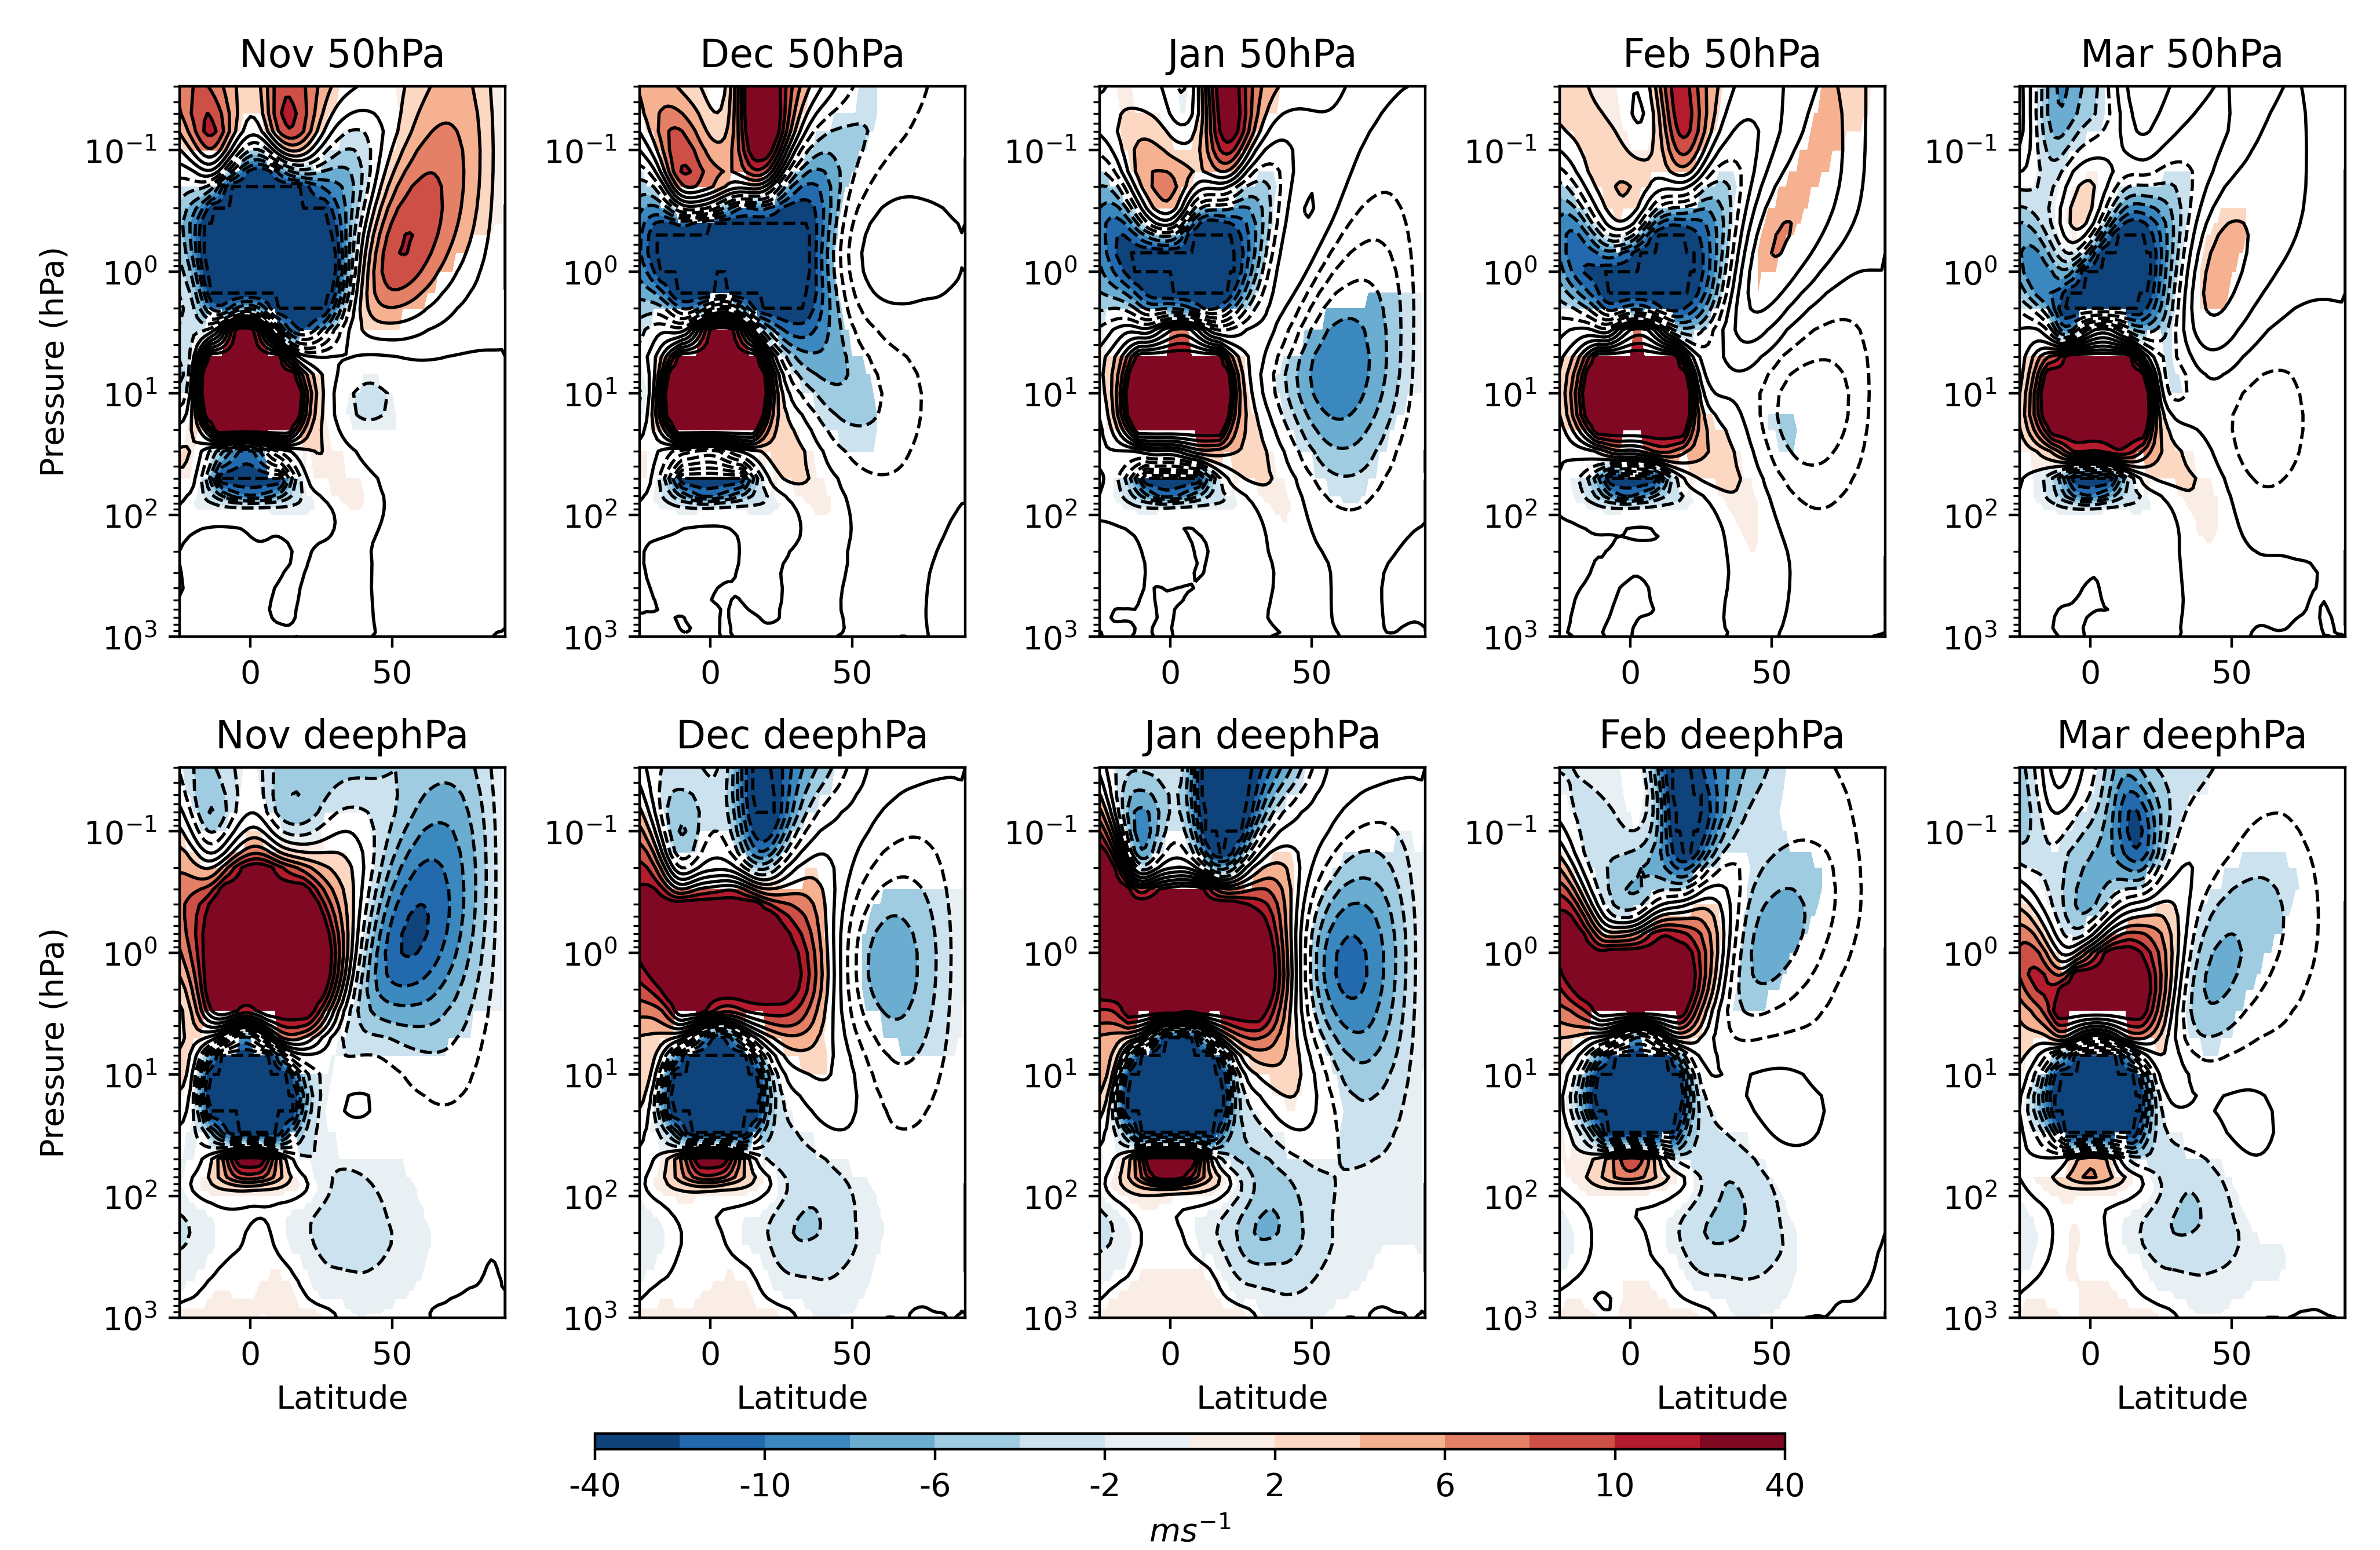
\includegraphics[width = \linewidth]{Figures/Figures-deepQBO/LAGGED_ZMZW_composites_by_month_QBO_phases_U_picontrol_MarQBO_vs_Mar_deephPa_5thresh.png}
\caption[ZMZW composites under different QBO phases in the pi-control simulation]{ZMZW composite differences for QBOE - QBOW from for the pi-control simulation of UKESM. QBO phases are defined using the Nov-Dec equatorial ZMZW on the 50 hPa level (top row) and the same deep metric as employed in \cite{andrewsObserved2019d}, the monthly equatorial ($5^{\circ}$\ S--$5^{\circ}\ $N average) ZMZW averaged between the 15 hPa and 30 hPa levels (bottom row). Differences are evaluated in a range of NH winter months (indicated in sub-figure titles). Coloured shading indicates ZMZW differences significant above the 95\% confidence level under a 2 tail student’s t-test.}
\label{fig:HT_picontrol}
\end{center}
\end{figure}

There are also some significant anomalies in the equatorial USLM in both the single level (50 hPa) composites and the deep QBO composites in figure \ref{fig:HT_picontrol}. While they both show QBOE minus QBOW differences, the vertical structure of the equatorial anomalies is very different, because of the different levels used in the composite selection: 50 hPa vs 15-30 hPa. Both composites have a four-fold anomaly structure in the vertical at equatorial latitudes but they have opposite polarities. For example, the deep QBO composite defined at 15-30 hPa has a positive anomaly in the lowermost stratosphere while the single-level composite defined at 50 hPa has a negative anomaly in this height region. The fact that the deep QBO composite has a stronger and longer lasting HT response of the expected sign at high latitudes suggests that this lowermost anomaly is not important in determining the HT response (because the equatorial anomaly there is westerly but the vortex response is to weaken). This suggests that the HT response is more likely a complex response to the whole vertical wind structure over the equator. This has been noted previously, in the context that planetary waves are deep structures and most likely are influenced by the equatorial winds over a significant depth of the stratosphere and possibly even the lower mesosphere. However, with such a complex vertical structure, it is not possible to isolate the most important height region. Returning to the idealised experiments, the deep experiment had a simpler two/three-fold structure in the vertical that suggested the equatorial USLM winds were most influential in determining the sign of the high latitude HT response, since easterly winds in the USLM led to a weaker vortex, and vice versa. Nevertheless, without a better understanding of the HT mechanism it is still not clear which is the most important influence i.e. whether the response depends upon the amplitude of an anomaly, the height region of an anomaly or maybe even the location / strength of the vertical wind shear (or perhaps some combination of these). While these simulations help to point to a possible influence from the equatorial USLM region, further experiments and analysis are needed to confirm this.

\section{Summary and discussion}
In this chapter, we analysed the influence of vertical structure of the QBO in teleconnections with the vortex and surface using a set of relaxation experiments which prescribed different degrees of QBO vertical coherence. While many studies have suggested the importance of QBO metrics which incorporate the vertical structure of the QBO \citep{schenzingerDefining2017, graySurface2018b, andrewsObserved2019d}, many of them identify statistical associations between QBO metrics and other climate variability but encounter problems proving causality in teleconnections. As a result, the true nature of QBO teleconnections including many of the mechanisms involved are still not fully understood. 

We found that an un-nudged configuration of the model (the pi-clim cntrl) was able to simulate some elements of connection between the QBO and the surface however the MSLP response patterns did not closely resemble that of the NAO or AO and were significantly less coherent and persistent than those reported in previous modelling and observational studies (namely \cite{andrewsObserved2019d}). A simulation which prescribed a QBO with perpetual vertical coherence (the deep QBO experiment) exhibited significantly larger anomalies in MSLP than both the un-nudged simulation and one that prescribed a shallow QBO (with different QBO phases near the 100 hPa and 10 hPa levels respectively). These large anomalies in the deep experiment corresponded to an NAO pattern in late NH concentrated over the southern node in the Azores region. Surprisingly, QBOE phases were associated with a positive NAO pattern, an opposite response to that found in studies using a deep QBO metric \citep{andrewsObserved2019d} as well as that expected from a pathway involving the vortex and the Holton-Tan association \citep{HoltonJamesRTan1980}.

We aimed to account for this opposite sign in QBO responses by examining the vortex response to QBO phases in each experiment. As with the MSLP response, the deep QBO experiment shows larger magnitude vortex responses from the vortex to QBO phases (figure \ref{fig:HT_deep}) than in the shallow and un-nudged simulations (figures \ref{fig:HT_piclim} and \ref{fig:HT_shallow}). These responses also evolve within the NH winter with negative response to QBOE in early winter (in line with an expected HT link) and large amplitude positive responses in Jan-Mar. This switch in vortex response may account for the NAO patterns in late winter; the positive vortex response to QBOE in later winter leads to a positive NAO via the vortex's influence over the NAO \citep{charlton-perezInfluence2018e}. 

Additionally, we noted that the late winter vortex response in this deep experiment (which was largely absent in the other experiments) were associated with significant SAO anomalies, likely induced via preferential filtering of equatorial waves by the deep QBO phase below. In the same simulation, the vortex was shown to respond to variations in the USLM QBO and an analysis of EP fluxes revealed that anomalies in the easterly phase of the SAO associated with different QBO phases were also associated with anomalies in equatorward propagation of planetary waves in the upper stratosphere. This lead to reduced wave driving of the vortex under QBOE conditions and a strengthening in late NH winter. This gives a potential mechanism by which later winter MSLP response patterns correspond to positive (negative) NAO under QBOE (QBOW) however it is unclear whether the vortex anomalies drive the SAO variations or vice versa.

A comparison of responses to the QBO in our deep nudged experiment with the use of a deep QBO metric in a free-running pi-control (similar to that used in \cite{andrewsObserved2019d}) highlighted a number of key differences: The sign of the HT link and MSLP responses were consistent with previous work in the pi-control and the equatorial anomalies induced by the QBO Exhibited a different four-fold structure as opposed to the two-fold pattern in height exhibited by responses in the deep nudged experiment. There is a possibility that the perpetually deep QBO in our experiment acted to perturb the equatorial ULSM region with an unrealistic structure of anomalies which, in turn, lead to large magnitude responses in the vortex and MSLP of the opposite sign to a HT link. However, showing this connection explicitly is challenging with the simulations analysed here and further targeted experiments are required to study this effect more closely. Nevertheless, this feature provided further evidence of the role of the USLM QBO in vortex variability (in agreement with \cite{grayForecasting2020a}). 

Overall, our experiments suggest that elements of QBO teleconnections are enhanced by the presence of a perpetually deep QBO: In early NH winter (Nov), the deep experiment's vortex responses to the QBO (figure \ref{fig:HT_deep}, 1st column) is negative under QBOE phases (consistent with the expected HT link) and significantly larger compared to the presence of a perpetual shallow and freely evolving QBO (the pi-clim cntrl). This result may confirm the findings of works highlighting the importance of QBO vertical structure for the HT link (e.g. \cite{graySurface2018b}) as well as provide a stronger case for causal teleconnections with the use of relaxation experiments. However, the enhanced early winter vortex response is not reflected in the November MSLP responses which was a key result in \cite{andrewsObserved2019d} so our results do not fully corroborate all previous work regarding this link. Furthermore, mid-late winter teleconnections (both MSLP and vortex) appear inconsistent with previous work in our deep experiments as our deep QBO induces large USLM anomalies which modulate the vortex response and obscure the signal from other pathways. 

To overcome this, further relaxation experiments which impose a deep or shallow QBO and also constrain the SAO winds may be useful. For example, repeating the deep QBO experiment but with a vertical extension of the relaxation into the USLM where winds were nudged towards either climatological ZMZW from a different simulation or using a reanalysis product. These simulations would eradicate the large USLM responses to QBO phase and isolate the effect of vertical QBO structure on teleconnections through other possible pathways. For example, the subtropical route suggested by \cite{graySurface2018b} was prominent in the deep experiment (figure \ref{fig:HT_deep}, below the 100 hPa level) but whose effect was obscured by the SAO anomalies and subsequent vortex and MSLP response. Biases in the underlying model for each experiment may also influence our results: Each simulation, similarly to the pi-control, exhibit a significant number of November SSWs. This has the potential to alter the evolution of the vortex throughout the remainder of winter as the vortex recovers from a November disruption. However, these November warmings occurred at similar rates in all experiments and we accounted for this bias by testing the sensitivity of results to removing years containing a November SSW finding that the key features of QBO responses were generally unaffected.

A similar limitation to our approach in this analysis is the fact that perpetual deep or shallow QBO conditions may not be fully representative of the real climate system - Reanalyses exhibit a QBO with deep and shallow attributes at different times and composite analysis which samples conditioned on the appearance of these characteristics produces coherent teleconnection patterns \citep{andrewsObserved2019d}. Where possible, we have imposed reasonable charactersitics in both the deep and shallow QBOs; their descent rates, for example, were chosen within a range from an observational study \citep{kinnersleyDescent1996} and the period was selected in line with the pi-control and pi-clim cntrl for ease of comparison. Nevertheless, our simulations are designed to isolate the effect of these structures on teleconnections from noise in the climate system and, to this end, their representation may not fully mirror that of the real atmosphere. If carefully designed, targeted sensitivity experiments such as ours remain a useful tool to examine causality between features in the QBO and extra-tropical variability.
